% EPL master thesis cover template
\documentclass{eplmastersthesis}

% help package for todo
\usepackage{xargs}                      % Use more than one optional parameter in a new commands
\usepackage[pdftex,dvipsnames]{xcolor}  % Coloured text etc.
% 

\usepackage{moreverb}
\usepackage{hyperref} % for url and so on
\usepackage{glossaries}
\usepackage[colorinlistoftodos,prependcaption,textsize=tiny]{todonotes}
\newcommandx{\unsure}[2][1=]{\todo[linecolor=red,backgroundcolor=red!25,bordercolor=red,#1]{#2}}
\newcommandx{\change}[2][1=]{\todo[linecolor=blue,backgroundcolor=blue!25,bordercolor=blue,#1]{#2}}
\newcommandx{\info}[2][1=]{\todo[linecolor=OliveGreen,backgroundcolor=OliveGreen!25,bordercolor=OliveGreen,#1]{#2}}
\newcommandx{\improvement}[2][1=]{\todo[linecolor=Plum,backgroundcolor=Plum!25,bordercolor=Plum,#1]{#2}}
\newcommandx{\thiswillnotshow}[2][1=]{\todo[disable,#1]{#2}}

% Fill in here the information: title, student name, speciality, jury members
\title{Privacy Aware Sharing of IOCs in MISP}	% Master thesis title
%\subtitle{Subtitle (optional)}			% Optional subtitle
\author{Charles \textsc{Jacquet}}	% Student name
%\secondauthor{Firstname \textsc{Lastname}}	% Second student name if applicable
\speciality{Computer Science and Engineering}		% Speciality (use one of the following options):
										% Biomedical Engineering
										% Chemical and Materials Engineering
										% Civil Engineering
										% Computer Science
										% Computer Science and Engineering
										% Electrical Engineering
										% Electro-mechanical Engineering
										% Mathematical Engineering
										% Mechanical Engineering
										% Physical Engineering
%\options{Option(s)}		% If required by program commission mention options
\supervisor{Ramin \textsc{Sadre}}	% 1st supervisor name
%\cosupervisor{Firstname \textsc{Lastname}}	% 2nd supervisor name if applicable
\readerone{Antoine \textsc{Cailliau}, Alexandre \textsc{Dulaunoy}}		% 1st reader name
\readertwo{William \textsc{Robinet}}		% 2nd reader name
\readerthree{François-Xavier \textsc{Standaert}}	% 3rd reader name
\years{2016-2017}	% Academic year

\newacronym{misp}{MISP}{Malware Information Sharing Platform and Threat Sharing}
\newacronym{ioc}{IOC}{Indicator Of Compromise}
\newacronym{kdf}{KDF}{Key Derivation Function}
\newacronym{pbkdf2}{PBKDF2}{Password-Based Key Derivation Function 2}
\newacronym{hmac}{HMAC}{keyed-Hash Message Authentication Code}
\newacronym{aes}{AES}{Advanced Encryption Standard}
\newacronym{csv}{CSV}{Comma-separated values}
\newacronym{tsv}{TSV}{Tabulation-separated values}
\newacronym{url}{URL}{Uniform Resource Locator}
\newacronym{ipv4}{IPv4}{Internet Protocol version 4}
\newacronym{ipv6}{IPv6}{Internet Protocol version 6}
\newacronym{uuid}{UUID}{Unique Universal Indentifier}
\newacronym{fp}{FP}{False Positive}
\newacronym{pprl}{PPRL}{Privacy-Preserving Record Linkage}
\newacronym{ip}{IP}{Internet Protocol}
\newacronym{osint}{OSINT}{Open Source Intelligence}
\newacronym{isao}{ISAO}{Information Sharing and Analysis Organisation}
\newacronym{dhs}{DHS}{Department of Homeland Security}
\newacronym{taxii}{TAXII}{Trusted Automated eXchange of Indicator of Information}
\newacronym{stix}{STIX}{Structured Threat Information eXpression}
\newacronym{cybox}{CybOX}{Cyber Observable eXpression }
\newacronym{coa}{COA}{Course Of Action}
\newacronym{nist}{NIST}{National Institute of Standards and Technology}
\newacronym{ids}{IDS}{Intrusion Detection System}
\newacronym{ips}{IPS}{Intrusion Prevention System}
\newacronym{api}{API}{Application Programming Interface}
\newacronym{rfc}{RFC}{Request For Comments}


\makeglossaries
\begin{document}

\maketitle					% To create front cover page
\thispagestyle{empty}		% To suppress header and footer on the back of the cover page


\begin{abstract} 
Malwares are plaguing this computer age. An actual solution to protect computer systems against them is threat information sharing: Organisations share lists of Indicators Of Compromise with each other.\\
For that, an interesting open source platform called MISP allows companies to share these IOCs but also malware analyses and attack correlations in an online fashion.\\
On the other hand, offline lookup would also be an important feature but is stopped by the need of data privacy and confidentiality. This master thesis looks for sharing the dataset of IOCs while still protecting privacy and confidentiality by not directly disclosing the information. \\
After a state of the art, a possible found solution had been implemented with  some improvements before finally being analysed.
\end{abstract}


\renewcommand{\abstractname}{Acknowledgements}
\begin{abstract}
\todo[inline]{TODO}
\end{abstract}

\tableofcontents

\chapter{Introduction}
%\section{Interaction with this Latex Document (To be removed)}
%In order to facilitate comments, I've added some new commands explained by\footnote{http://tex.stackexchange.com/questions/9796/how-to-add-todo-notes}:\\
%\begin{itemize}
%\item unsure => What I need to check
%\item change => What have to be modified
%\item info => Add simple comment
%\item improvement => Indicate a possible improvement
%\end{itemize}

%Ponemon Institute conducts independent research on privacy, data protection and information security policy
In the last reports of the Ponemon institute\cite{ponemon2016cost, ponemon2016costFr}, the estimated cost of the annual data breaches for 384 companies in 12 countries\footnote{United States, United Kingdom, Germany, Australia, France, Brazil, Japan, Italy, India, the Arabian region (United Arab Emirates and Saudi Arabia), Canada and, South Africa} is about \$4 million each in 2016.\\
A data breach means that records containing private data linked to a name had been leaked. This originates from system glitches, human errors but  mostly from malicious and criminal attacks. In France, the percentages are respectively 23\%, 27\% and 50\% which gives an average cost of \$1.85 million a year only for criminal attack.\\
This cost mostly comes from business losses due to the lack of confidence resulting from a data breach. Unfortunately, it is growing from year to year and it will probably continue to increase as the global annual cybercrime costs predicted by Cybersecurity Ventures will grow from  \$3 trillion in 2015 to \$6 trillion by 2021.

Companies thus need to protect themselves against business losses and thus against cybersecurity threats by increasing their computer system defences. By that, it also means being able to improve the reactivity to new threats as they appear faster and faster which results in a delay for standards malware detection systems. Another important characteristic to notice is that analyses showed that the same attack vectors are used against the same type of organisations as they generally use the same kind of systems. From that, the idea of making correlations between trusted organisation arose and gave birth to threat sharing.  As soon as an organisation discovers a threat, they can prevent others to be compromised just by informing them about it.\\

For helping information sharing, a lot of tools appeared like standards (\gls{nist}, ENISA, ...), guidelines to involve an organisation in information sharing group but also platforms. One of them is called \gls{misp}. It allows organisations to share information like \gls{ioc}, analyses of the compromises and correlations between events.\\
This platform is mostly used in an online fashion with a direct access to the web interface or available \gls{api}.\\
But on the other side, it could be really useful to go one step further and allow to directly share the data set. It could have a lot of uses like for sharing information between \gls{misp} instances, for incidence response team, forensics, later offline lookups, ...\\
Unfortunately, a large wall stands between the idea and its realisation: the combination of privacy and confidentiality needs.\\ 
A technique is therefore required for \textbf{sharing} information without \textbf{disclosing} damageable information to other parties. This master thesis works on finding a "more secure" way of sharing an encrypted database of these \gls{ioc}s in order to protect the data by slowing down as much as possible a brute force attack while still making this database useful for the targeted users.\\

The first chapter is to learn about the used concepts. A brief overview of the recent works and of the state of the art follows.\\
After that, an explanation of existing techniques will allow understanding the advantages but also disadvantages of the possible tracks to follow.\\

The last chapters are about the implementation, tests, and results obtained.\\
Finally, I will conclude on my work with some possible improvement and future works and discussions.

\section{Organisation}
Before going deep into the subject, I want to point out some aspects of the this project development.\\
Firstly, last year, I was searching for a security subject but I was not really excited about the proposed ones. On the other side, I had no idea either on what I could work in cybersecurity. Therefore, I've looked for ideas where there are plenty of them, directly in security companies.\\
I've found a company called Conostix which provides security and system services in Luxembourg.\\
They weren't short of ideas. Later on, William Robinet (from Conostix) contacted me again to say that they have a better idea and it was to work on \gls{misp}. I've thus met Alexandre Dulaunoy from CIRCL with William and they gave me the starting point of the project which was malware sharing in \gls{misp}.\\

As I had zero knowledge in this domain, I've chosen to make an internship of four weeks in the company (not credited) where I've learned the basics of \gls{misp}. I've also worked on network log parsing. But what I mostly learned was that four weeks for trying to specialise myself in a completely new domain was only enough to give me a rough idea of what it is.\\
During these four weeks, I mostly worked on logs. I've created nothing new, actually, it was quite the opposite but it was still interesting to understand how things were working and why they could be useful. \\
In short, I have started to understand how the proxy squid3 was working and have installed it on my computer in order to get logs to work on.\\
Once done, I tried to get information from them by manually parsed the logs (which was a mistake). For that purpose, I've started to implement a parser that was using regular expressions to transform each log lines into a set of objects. But even if it was funny to implement, I spent a lot of time on it and each time I finished, I found it to be not good enough, not modular enough, losing locality and ordering information, and so on. I have thus realised that I was loosing my time as of course, they are plenty of tools for this kind of job like the later used Logstash.\\
Then I've started to work with \gls{misp} to see how it was working. I've reimplemented a similar hash store like the misp-workbench project.\\
I've then used it with my log system by parsing the data from \gls{misp} before adding them to the hash database on Redis.\\
I've then created a way to feed the parsed logs in my system and briefly analyse them.\\
Besides that, I also had the opportunity to benefit from a one-day \gls{misp} training organised by CIRCL.
I have then continued to work on my master thesis the whole year long while keeping in touch with Conostix and CIRCL.

\chapter{Background}
This small chapter is intended to give a quick overview of the tools and concepts on which this master thesis is based.

\section{Indicator of Compromise (IOC)}
When there is a crime, detectives come and look for clues. They do that to answer important questions as why it happened and also how it happened. This is really important, not only for solving a specific crime but also for gathering information that could allow solving other correlated crimes and perhaps avoid other similar ones as well.\\
This is exactly the same idea here, even if the attacker try to minimise its traces, there are always some. It can be email addresses, \gls{ip} addresses, malware, \gls{url} and so on.\\
The idea is then to use these traces to trigger alarms on other computer systems as soon as they are seen to protect them as well as gathering new information. This is the reason why we call these type of clues Indicator Of Compromise.

\section{Confidentiality and Privacy}
These two terms are used a lot and nearly in an interchangeable way in this master thesis. But it is still important to look more closely at the difference of meaning between those two terms at first.\\

Confidentiality is related to confidence, we entrust others with our information even if they could affect us by revealing it to non-authorized people. Confidentiality is a right in some health domain like medicine and so on but is also requested by companies when they accept sharing information.\\

Privacy, on the other hand, is that we don't want to be investigated more on what we share. This is not because we give the finger that the arm could be taken.


\section{MISP and Threat Sharing}
I've introduced the idea of malware sharing to defend computer systems against digital threats and attacks. But \gls{misp} is not the only platform to do so, current ones are DShield, Critical Stack’s Intel, Microsoft’s Interflow, AlienVault’s Open Threat Exchange, ThreatExchange (Facebook).\\
But here I focused only on the \gls{misp} project which is, as said on their website, an open source software solution for collecting, storing, distributing and sharing cybersecurity indicators and threat about cybersecurity incidents analysis and malware analysis. \gls{misp} is designed by and for incident analysts, security and IT professionals or malware reverser to support their day-to-day operations to share structured information efficiently.\\
\gls{misp} rely on an hub and spoke sharing model (\gls{taxii} \cite{taxiiWebsite}). There is a central point called the hub which is the server responsible for a \gls{misp} instance, where all data are kept, and the spokes are the organisations that interact with the hub.\\
A recent paper on \gls{misp} \cite{wagner2016misp} had been published this year and could be interesting to get a better understanding of the underlying system. Additionally, there is also a recent ietf draft on the \gls{misp} core format\cite{MispDraft}.\\
I want also to point out that \gls{misp} is spreading, and I've the feeling that communities will continue to grow. I've discussed in Belgium with companies like banks, insurances, consultancy companies that are using it, I've even met people knowing it when I was in Singapore for the Black Hat Asia conference (2017). All this is, at least to my point of view, a good sign on the utilisation of the system.

\subsection{History}
As explained on the \gls{misp} project website, Christophe Vandeplas started the project as he was tired of the way IOCs were shared (email, pdf, ... ). Hence he created a cakePHP website as a proof of concept and managed to convince the Belgian Defence (where he was working) that the project was worth it. They even allowed him to work on it during his work-hours. At that time, the project was named CyDefSIG: Cyber Defence Signatures.\\

Then NATO heard of it and got the first presentation in January 2012 to introduce in more depth the project and they started to invest themselves into the project. Andrzej Dereszowski was the first part-time developer from NATO side.\\
One thing led to another and some months later NATO hired a full-time developer to improve the code and add more features. A collaborative development started from that date. \\
It was collaboratively decided at that time that the project would be released publicly under the Affero GPL license. This to share the code with as many people as possible and to protect it from any harm.\\
The project was then renamed to \gls{misp}: Malware Information Sharing Project, a name invented by Alex Vandurme from NATO.\\
In January 2013 Andras Iklody (initially hired by NATO) became the main full-time developer of \gls{misp}.\\

Meanwhile other organisations started to adopt the software and promoted it around the CERT world. (CERT-EU, CIRCL, and many others …)\\
Nowadays, Andras Iklody is the lead developer of the \gls{misp} project and works for CIRCL.\\

\subsection{Basics of MISP}
The idea of \gls{misp} was first to create an \gls{ioc} database. That is, if there is an attack where \gls{ioc}s had been seen: "IOC@malware.mail" and "192.168.16.2". We need to keep two types of information, the two \gls{ioc}s by themselves but also the relation between them. For expressing the later one, \gls{ioc}s are grouped by event, a more general term than "attack" previously used in this work.  Then, the \gls{ioc}s, are considered as the attributes of the specific event representing that particular attack.\\
This representation is quite efficient to analyse as it can immediately correlate events thanks to their attributes.\\

For clarity concerns, attributes are divided into 13 categories again divided into types. As \gls{misp} is not anymore limited to malware, it is interesting to notice that we can also see categories like Financial Fraud but more standard ones are Network Activities, Antivirus detection, Artifacts dropped, and so on.\\
All the categories and types can be found on their web pages\footnote {\url{https://www.circl.lu/doc/MISP/categories-and-types/index.html}}

One other really interesting feature is sightings. When an \gls{ioc} is referenced, we know that it has been seen by someone, but it does not confirm that the \gls{ioc} is really related to that particular event and is not an error. Moreover, what says that if a dynamic \gls{ip} address is an \gls{ioc} today that it is going to be the case in 3 months? \\
Sightings is thus the solution to this problem as we can monitor an \gls{ioc}, knowing if it has been seen at other places and if they are still relevant.


There are also two important things on the sharing strategy that I want to point out: \gls{misp} instances and communities. The first one is easy to understand, \gls{misp} is an open source project which means that everybody can decide to run a completely isolated \gls{misp} instance for its own needs. For example, a company that want to store its own confidential data. But that does not mean that the instance \textbf{must be} isolated, they have implemented a way to share information between these instances. While the second one is a good property of each instance, when connected to \gls{misp}, a user is connected thanks to the organisation he belongs to. Then, the organisation can choose to share or not to share their events/attributes with other communities or even with other instances. \\ 

\gls{misp} became a really good \gls{ioc} database with automated correlation system. These correlations can be represented under the form of a graph that helps the analyst to visually see connections.\\

Besides all that, a lot of different tools had been implemented like a python client library and are available on their repository: \url{https://github.com/MISP/}.\\
They have also added a lot of plugins to the web interface like the ability to export the attributes in different formats, standard ones and some other for specific \gls{ids}.\\

\subsection{My Settings}

\gls{misp} is really easy to use, but if we want to go deeper in it, there are a lot of things to understand. That's why they give training and make available a \gls{misp} training virtual machine in order to train ourselves and test new developments.\\
At the beginning, I've started to work on a private instance of \gls{misp} hosted by CIRCL but, every time that I was working, I needed to have a really good web connection to download all the data. That's why I finally downloaded the virtual machine. 
The MySQL database was not accessible from outside the virtual machine but, as I was going to work on my computer and I didn't want to be stuck programming inside the virtual machine, I've done some modifications to make available the database to my local network.\\
The first step was to check that my virtual machine runs using the virtual vboxnet0 interface (Standard interface used for a network only between hosts and the hypervisor for Virtualbox) and was using the \gls{ipv4} address 192.168.56.50. Normally it works without any problems but it didn't work on my computer, I thus added an \gls{ip} in the right range by using the command:
\textbf{ip add add 192.169.56.2/24 dev vboxnet0} .\\
I'm also sometimes using a second virtual machine to work with and on this virtual machine, I've configured two network interfaces, the first one was to have an internet connection while the second one was the vboxnet0 interface.\\
For simplifying the use of the vbox interface, I've configured my network to automatically add an \gls{ip} in the right range (/etc/network/interfaces). This is the addition to the basic configuration:
\begin{verbatim}
auto eth1
iface eth1 inet static
address 192.168.56.1
netmask 255.255.255.0
\end{verbatim}
 
After that, I was able to contact the virtual machine via the network but it wasn't enough to have a MySQL access. \\
Therefore, I modified the configuration file (/etc/mysql/my.conf or /etc/mysql/mysql.conf.d/mysql.cnf depending on the VM version) where I've just commented the "bind-address 127.0.0.1" line.
The next step was to create a user with the rights from the outside. For that, I've connected myself to the database as the \gls{misp} user and I've added the user:
\begin{itemize}
\item[•] mysql -uroot -pPassword1234 
\item[•] CREATE USER 'username'@'\%' IDENTIFIED BY 'Password1234';
\item[•] GRANT ALL ON *.* TO 'username'@'\%';
\end{itemize}

Once done, I could continue to program more easily and create some tests as I could control the whole available dataset.\\

\subsection{MISP in a few Pictures and the Traffic Light Protocol}
There is nothing better to explain all that than real screenshots of the web application. But, it raised one really important question: what can be shared from \gls{misp} and with whom?\\
For example, Am I allowed to show screenshots of data from \gls{misp} without any risk?\\
For answering that question, I need to introduce the Traffic Light Protocol (TLP) that was created in order to facilitate information sharing by defining the authorised level of disclosure. And thus, it can be used to know what can be shared with a specific audience.\\
This protocol is defined by FIRST in \cite{FirstTLP} but also explained in this \gls{nist} cyber threat information sharing guide \cite{johnson2016guide}.\\

With that I know that I can share the data from the virtual machine that I have explained in the previous section as the default \gls{osint} feed is TLP:WHITE. Which means, according to FIRST, that the disclosure is not limited: \\

\begin{boxedverbatim}
	Sources may use TLP:WHITE when information carries minimal or no foreseeable 
	risk of misuse, in accordance with applicable rules and procedures for public 
	release. Subject to standard copyright rules, TLP:WHITE information may be 
	distributed without restriction.
\end{boxedverbatim}

The main page of the web application (fig. \ref{webevents}) is a list of all latest events on figure \ref{webevents} (notice the "tlp:while" appearing in the Tags).

\begin{figure}[!h]
	\begin{center}
		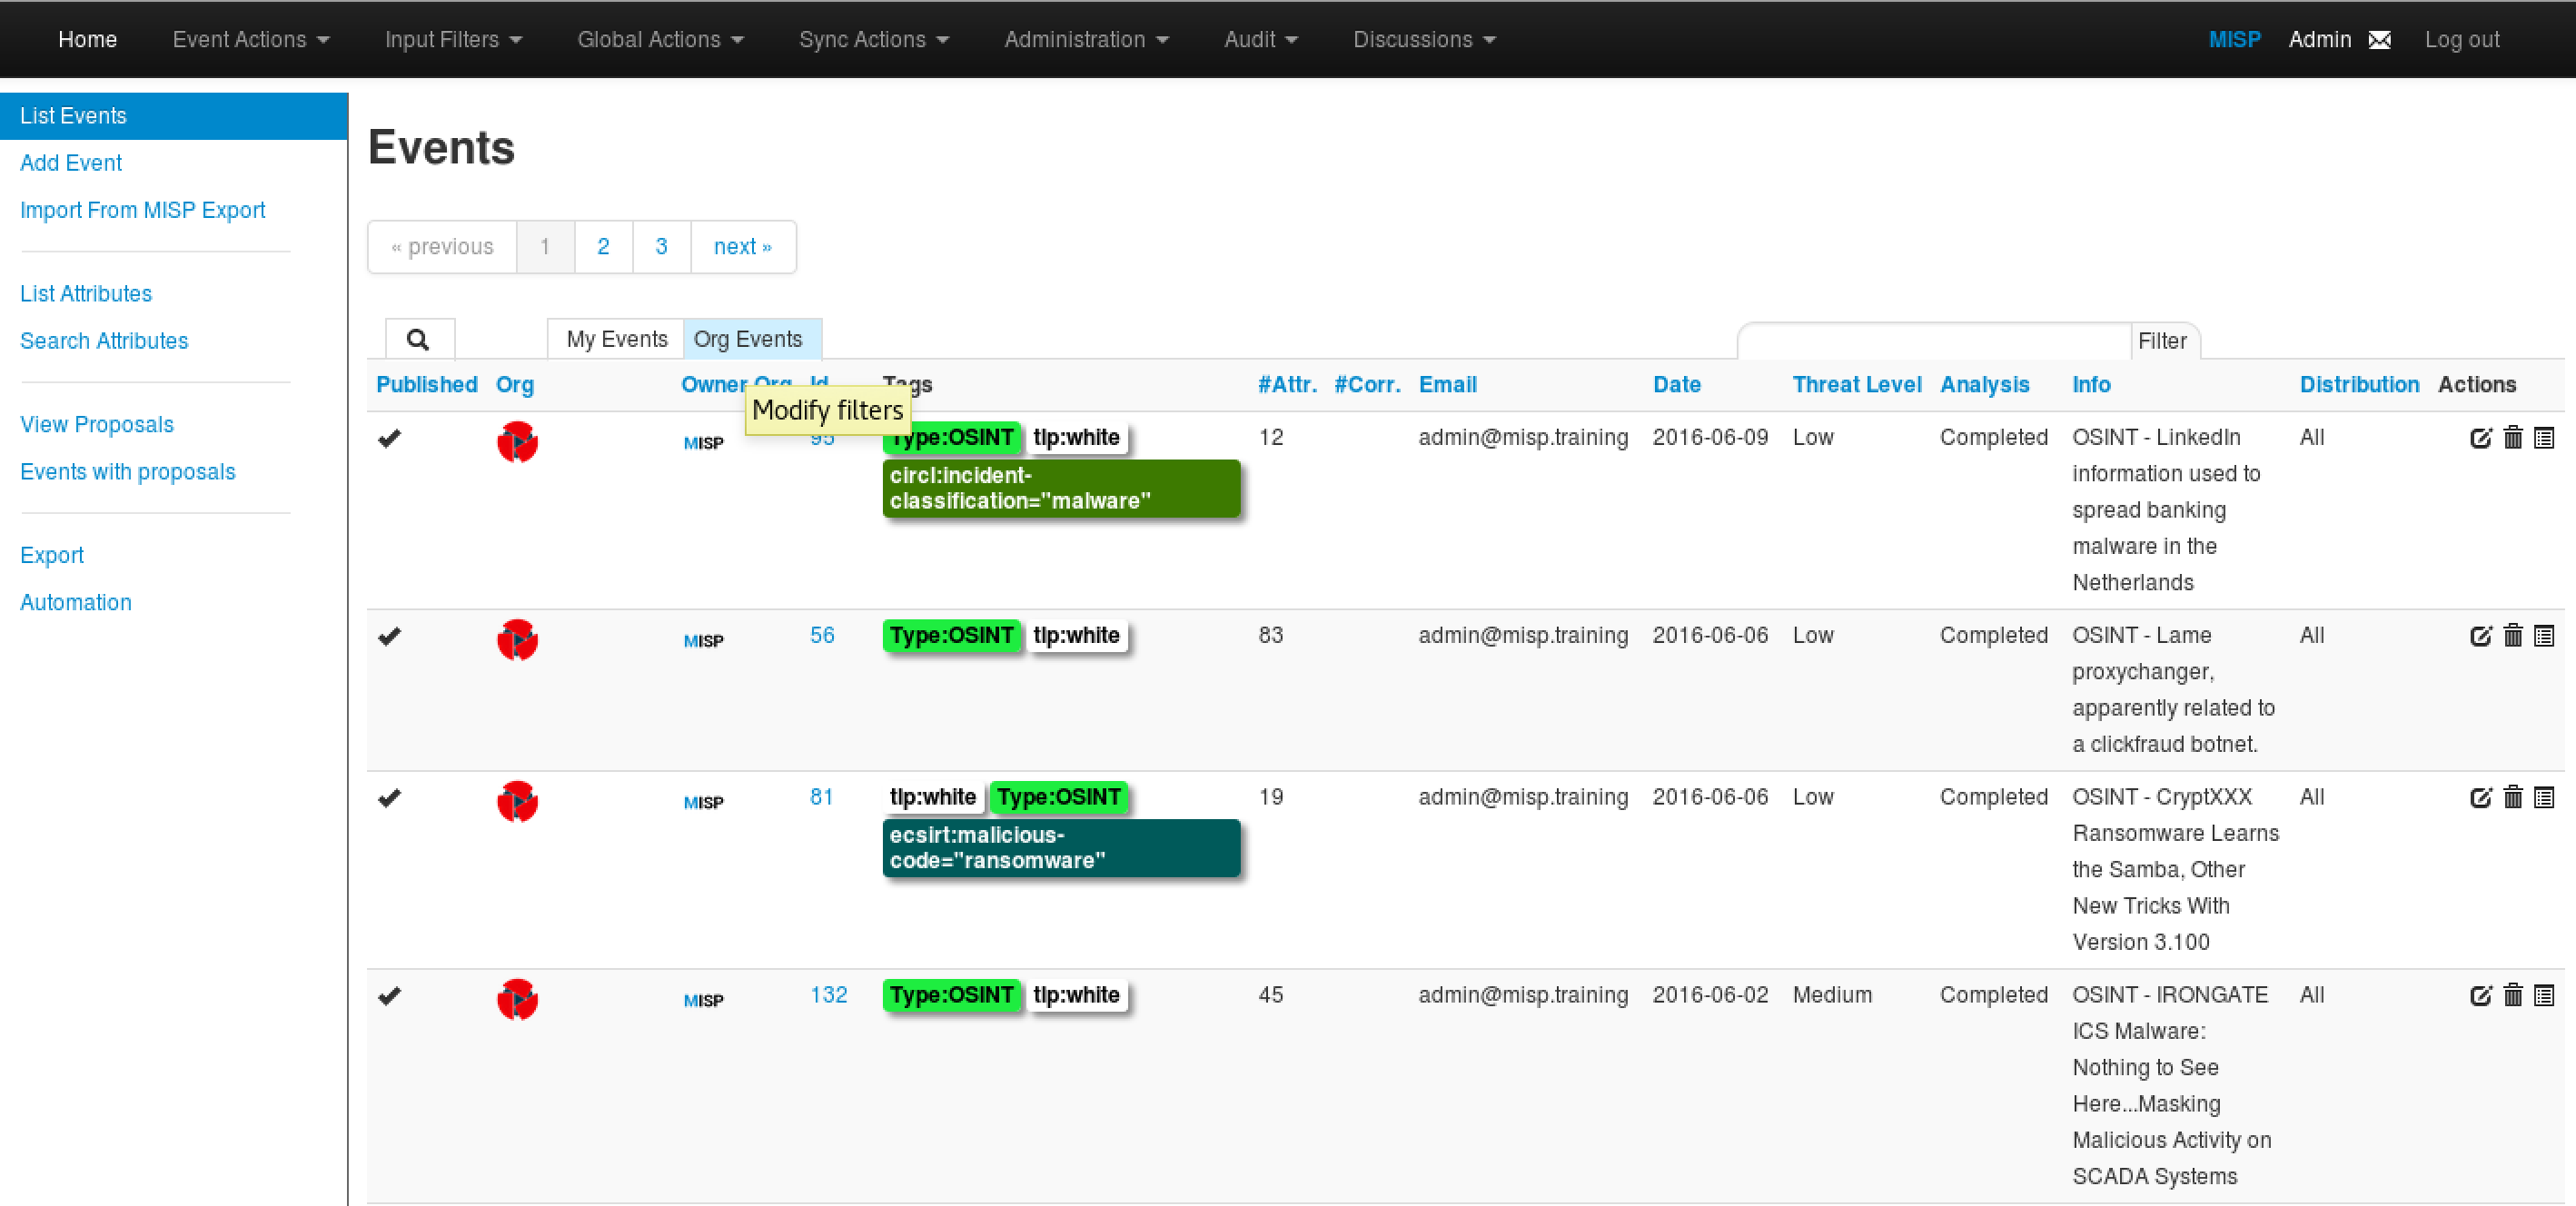
\includegraphics[scale=0.32]{res/webEvents}
		\caption{MISP : List of events}
		\label{webevents}
	\end{center}
\end{figure}


Then, by clicking on an event, we can get information on it (fig. \ref{webevent}).


\begin{figure}[!h]
	\begin{center}
		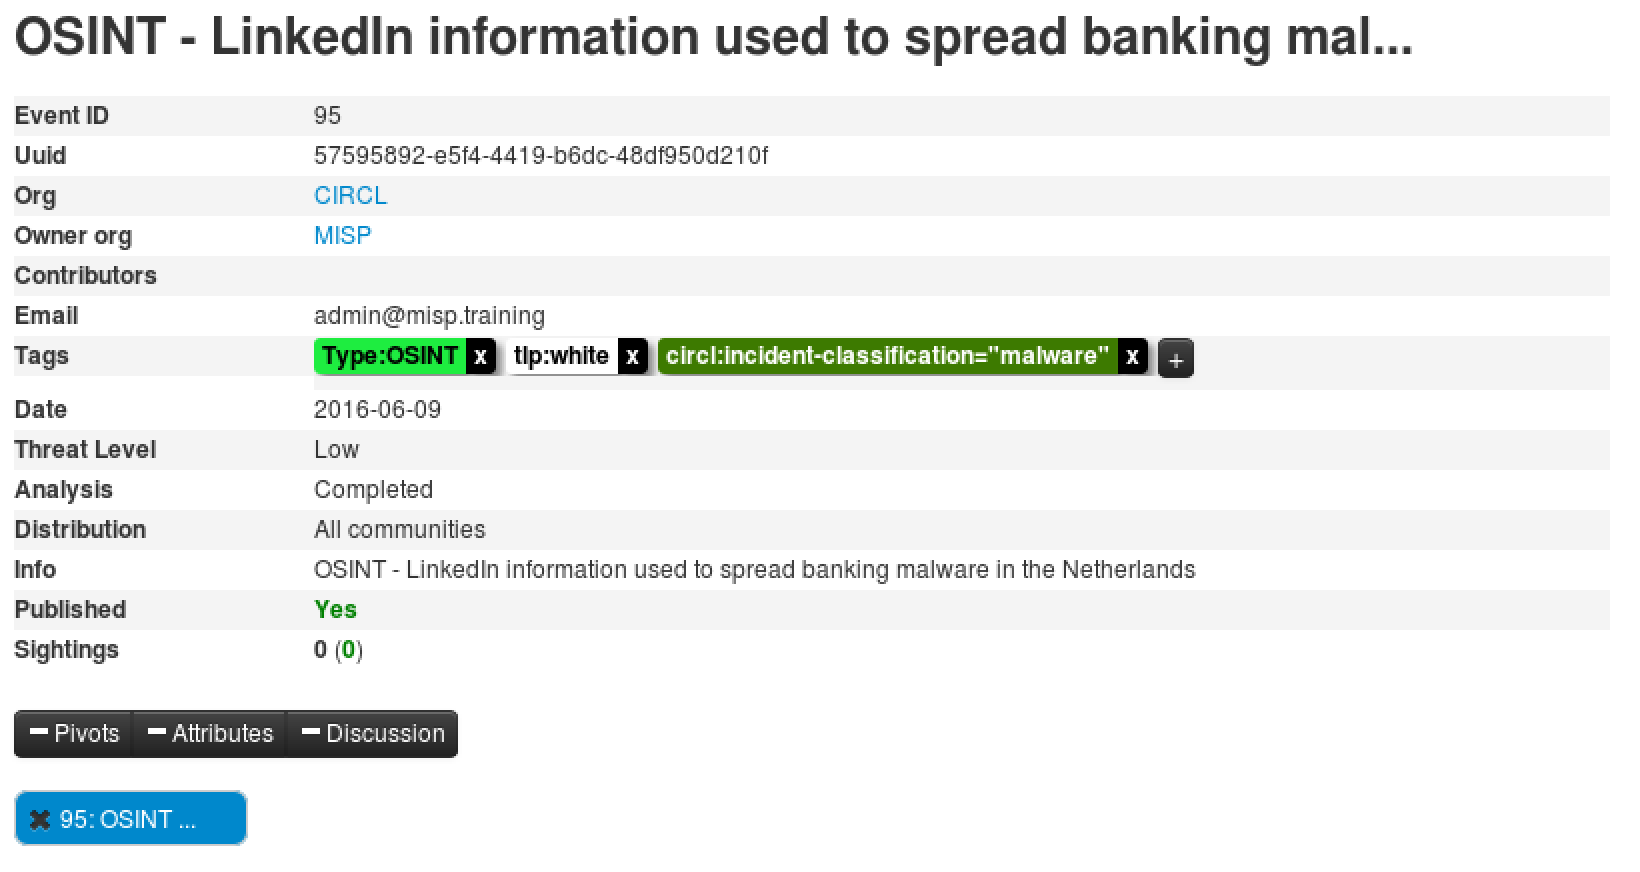
\includegraphics[scale=0.35]{res/webEvent}
		\caption{MISP : Specific information on the event}
		\label{webevent}
	\end{center}
\end{figure}


As well as the attribute list (fig. \ref{webattributes}).
\begin{figure}[!h]
	\begin{center}
		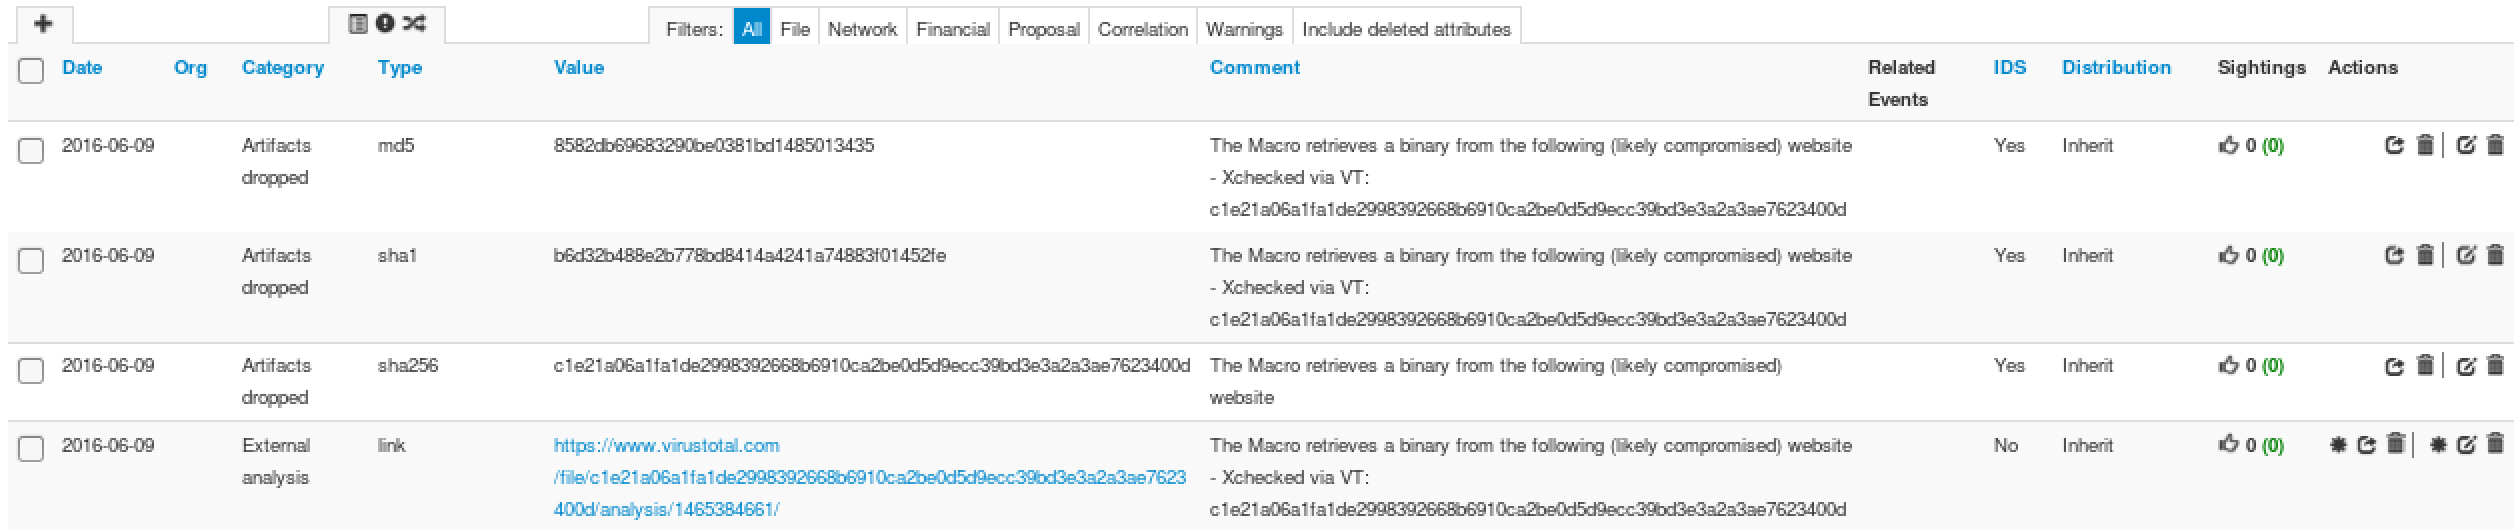
\includegraphics[scale=0.35]{res/webAttributes}
		\caption{MISP : Attributes of the event}
		\label{webattributes}
	\end{center}
\end{figure}

And the last thing that I want to show is one of the ways of showing the correlations with other events and is called the correlation graph (fig. \ref{webcorrelation}).
\begin{figure}[!h]
	\begin{center}
		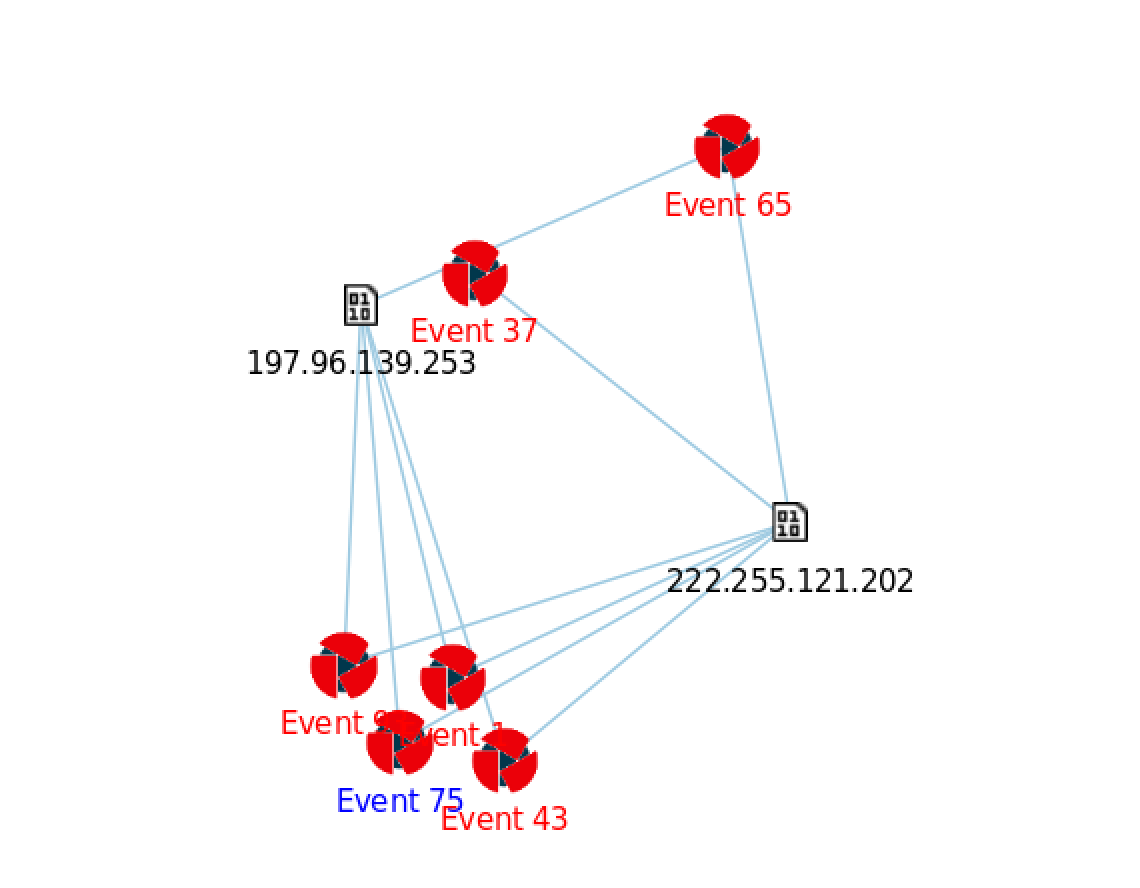
\includegraphics[scale=0.35]{res/webCorrelationGraph}
		\caption{MISP : Correlation graph for an event}
		\label{webcorrelation}
	\end{center}
\end{figure}

\subsection{Misp-Worbench - hashstore}

MISP workbench\footnote{https://github.com/MISP/misp-workbench} is a set of tools to export data out of the \gls{misp} MySQL database and use and abuse them outside of this platform.\\

CIRCL has already implemented a privacy aware tool called hashstore and implemented in redis\footnote{http://redis.io}. This is working by creating a dataset of all hashed \gls{ioc}s. And then by the use of the redis server, we can use a redis client to request data.\\
Like that, if you want an information on a particular \gls{ioc}, you need to already know it to be able to take its value's fingerprint and make the request.\\
On the other hand, coming back on the small data problem, if we consider an attacker that want to try every possible \gls{ip}s, for \gls{ipv4} it represents 4.228.250.625 different \gls{ip}s that needs to be tested. Even if it is a lot it is still feasible as redis is really fast. Moreover, not all \gls{ipv4} need to be tested, for an example we can avoid private subnet like 10.0.0.0/8, 172.16.0.0/12, 192.168.0.0/16 which already represent 17.891.328 addresses.


\chapter{Information Sharing State of the Art}

This chapter is aimed to give an overview of existing works in two domains, information sharing by itself and techniques used for privacy concerns.\\

\section{Information Sharing}
The chosen starting point is an already made state of the art about the subject done by Gregory White and Keith Harison in \cite{white2017state} where they explain the evolution of the information sharing by comparing it with the evolutions of the USA laws and their impacts.\\
Even if the analysis is about the USA, I believe it is important to understand the origin of the concept. For an example, to know that the first attempt of sharing standardisation was done just after the worm released by Robert Morris in 1988.\\
By analysing the impact of this worm, they rapidly realised that information sharing could have been a better and faster way to protect critical infrastructures. They also explain, in correlation with the two principal laws called the Presidential Decision Directive-63 in 1998 and the Executive Order 13636 in February 2013; how organisation like \gls{isao}s were created with their four foundational objectives that can be summarised as:
\begin{itemize}
\item[$\bullet$] Each organisation should be able to participate.
\item[$\bullet$] Development should be kept public.
\item[$\bullet$] Involvement should always be voluntary and should never be a requirement.
\item[$\bullet$] Take into account the need for confidentiality and privacy.
\end{itemize}
They also introduce the first sharing program developed by the \gls{dhs} which is the Cyber Information Sharing and Collaboration Program (CISCP).\\
With that, they introduce some standards like \gls{taxii}, \gls{stix} and \gls{cybox} explained in a few paragraphs. After that, they go through challenges that are facing the \gls{isao}s. The major one is a privacy and confidentially concern, any information that an organisation agrees to share with others, no matter who those others are, need to be kept private and confidential and only released to individuals or organisations that have a right to have access based on the agreements that are signed by members of an \gls{isao}. This concern is really interesting as this master thesis is really on trying to ensure that property without the need of trust. They also explained that privacy is that personal information about individuals within a member organisation should remain private (in the context of information sharing).
While confidentiality refers to information about organisation that could lead to give others a competitive advantage.\\
In this article, they focused a lot on trust which is one of the most important property to ensure when dealing with a sharing group as we cannot share confidential information if we do not trust the other party to keep it confidential and to respect privacy! \\

After that, a recent survey trying to compare the different vendors for threat information sharing was published in 2017 \cite{sauerwein2017threat}. The authors have conducted a systematic study of 22 threat intelligence sharing platforms and this article is a short sum up of their key findings I believe there is a lack of example to support their says, but it is still an interesting survey even if a detailed analyse of the 22 different tools would be really welcome.\\
On the other hand, their analysis of the different types, focuses, standards and licenses used by the different platforms brings a lot of information on what should be used in nowadays sharing platform.\\

I've introduced the name of some standards which are like language that we need to understand if we want the understand the meaning of what is shared. Therefore, it is these standards that make possible threat sharing but also allow to make it automated. Besides that, when we decide to start on this subject. It is really too important to avoid making mistakes that have already been made. That is why some organisations like the National Institute of Standards and Technology (\gls{nist}) and the European Union Agency for Network and Information Security (ENISA) took care of publishing guidelines to help organisations to involve themselves in threat sharing.\\
In Europe, the Commission recognised that they have a role to play in making the information more secure. In order to do so, they wanted to create the first pan European Information Sharing and Alerting System (EISAS on which we can find a report on the implementation \cite{eisasRapport}).  They consequently have asked to ENISA to define the requirements. Afterwards, member states that weren't yet using information sharing were really interested in and asked ENISA to develop a good practise guide based on the observation of existing exchange. This gave this guide \cite{enisaguide2009} aimed to assist member states but also relevant stakeholders like organisations using communication network and information systems in setting up and running network security information exchange.\\
In this guide, they go through setting up information sharing but they also took care of explaining the advantages as well as identifying laws that could get in the way. This is really important as organisations need to ensure themselves not being recognised as a cartel or that sharing becomes a commercial advantage. They also focused on the trust that is needed, for them, it must be created thanks to regular face-to-face meetings and TLP must be used as well during these meetings.\\
Then, in 2016, \gls{nist} also published its guide \cite{johnson2014guide} that seems to me more complete and more mature. This publication is also more focused on organisation than on States (unlike ENISA) and provides guidelines to improve cybersecurity operations and risk management activities through safe and effective information sharing practices.\\
For them, cyber threat information consists of \gls{ioc}s, TTP (tactic, techniques and procedures), suggested actions to detect, contain or prevent attacks and finally the findings from the analyses of incidents. \\
They go through different topics like the benefits and challenges encountered, how to establish and participate in sharing relations. Once again, they draw attention to the importance of trust and to be compliant with legal and organisational requirements among other challenges.\\

On another side, the paper written in February 2017 by Aziz Mohaisen et al. \cite{mohaisen2017rethinking} focus themselves on rethinking threat intelligence and to assess the risks. They argue by \cite{MalikThreat} that intelligence sharing is the only way to combat our growing skills gap in term of security. But they mostly claim that there are a lot of issues that needs to be explored in order to realise efficient and effective information sharing paradigms for actionable intelligence. They even go further by saying that understanding the risk of sharing as well as not sharing is absolutely needed for every organisation.\\
Briefly, not sharing is a risk as we don't receive information that could avoid us to be compromised. While on the other hand, sharing information without proper restrictions may leak a significant amount of information about participants and their operation context and all that can be used by an attacker to learn their vulnerabilities.\\
One of the commonly proposed solutions to that is to have a very limited sharing community only with highly trusted participants. But is it really what we need to do? If the participants are not enough, we could also not succeed in gathering enough information.\\
But, if we have less trusted participants, we also need to understand the risk of leakage that could lead to both monetary and reputation loss. Taking all that into account, they propose a new way of thinking for threat intelligence by defining models, communities and adversaries with their threat model.
They finally propose an architectural solution as a way of assessing the quality of sharing.

\section{Existing Techniques}
Then, It is interesting to see existing techniques used in information sharing to ensure privacy and confidentiality in a case where we do not want to rely on trust. These following paragraphs are used to discover what is used and what was used before in order to get ideas on what could be implemented.\\

The first idea is the simplest one and is about removing and hiding parts of the data. This technique is called data sanitization. Then there will be articles on secure two-parties (S2P) Computations and finally on \gls{pprl}.\\

One of the first articles that presents some concerns about privacy in sharing security alert is \cite{lincoln2004privacy}.
More precisely, they were concerned about protecting site-private topology, proprietary content, client relationship and site defensive capabilities or vulnerabilities.\\
This was done in two steps, the first one is data sanitisation, which consist in removing confidential data and useless information: Don't take the risk of revealing information to an attacker if this information is not needed by the user.\\
The second one is the correlation/aggregation work were alerts are linked together for analysis purpose.\\
 They have used three different categories of data coming from DShield and Symantec's DeepSight:
\begin{itemize}
\item Firewalls: They consider all "deny" as a possible attack
\item \gls{ids}: They remember logs of attacks that the \gls{ids} has found
\item Antivirus software
\end{itemize}

After removing all useless information, we can hash all confidential data. As the companies want to be ensured of the confidentiality, they assume this job of directly hashing the data before sending them to the server.
This technique is quite well working if, the data has a certain size. But, on the other hand, it is not useful for \gls{ip} addresses, if an attacker is targeting a company, it has to precompute only 256 or perhaps 65536 \gls{ip} address hashes. Thus this is not brute force resistant.\\
For each alert, we have two different \gls{ip}s, the source \gls{ip} (ip\_src) and the destination \gls{ip} (ip\_dest). We can classify all these \gls{ip}s in two categories:
\begin{itemize}
	\item Internal \gls{ip}s : \gls{ip}s that belong to the company
	\item External \gls{ip}s : \gls{ip}s external to the company
\end{itemize}

The first category is, of course, the one that we need to protect and in order to do so, these \gls{ip}s are hashed with a keyed hash function like \gls{hmac}. While the second type is only hashed by a simple hash algorithm like SHA-1.\\
The result is that we can compare all SHA-1 hashed \gls{ip}s together while only companies can decrypt their own internal \gls{ip} addresses.\\
An attacker cannot make the difference between an \gls{ip} hashed by \gls{hmac}  or SHA-1. Thus, for attacking the dataset, he would need to try to crack all \gls{ip}s as if they were SHA-1 fingerprints (For example with a TMTO attack). This, without forgetting that they receive millions of \gls{ip}s, makes it unfeasible for an attacker to brute-force the whole dataset.\\
They are also using another set of protections like the randomised threshold for publication of an alert but it goes out of the scope of this work.\\ 
In sanitization, they also round all timestamps to the nearest minute in order to add some uncertainty.\\
The second step is the correlation, they spoke about historical trend analyses, source/target-based analyses and event-driven analyses. These analyses worth spending time on them but are not related to the specific subject of this work.\\

Then, \cite{xu2005privacy} was also working on confidential data sharing starting from the first article, but they came up with a new interesting idea, instead of hashing confidential data, why not generalising it and doing probabilistic correlations.\\
The first idea was a guided alert sanitization with concept hierarchies. For example, if we have an \gls{ip} 192.168.1.123/32, we can generalise it to 192.168.0.0/16.\\
The depth of the generalisation is chosen thanks to the entropy or by the differential entropy technique explained in \cite{cover1991elements}.
\\
Then, for alert correlation, they focused on defining similarity functions between sanitised attributes and building attack scenarios from sanitised attributes\\
They also used a technique to create probabilistic attack scenario which is a set of alerts put together to create a bigger attack.\\

These articles were looking at data obfuscation while still being able to create correlation analyses but, it is difficult to apply it in order to create a database of still usable data for prevention or detection as it looses information.
\\

I've explained some solutions that can be applied to \gls{ip} addresses or file (like hashing them). But, what if we could do the same with all network packets and still getting some privacy!\\
That's the goal of \cite{parekh2006privacy}. Today, it's not good enough to analyse \gls{ip}s, \gls{url}s and so on. We need to go deeper in it, that's why they propose a technique based on the byte distribution of the packets.\\
They used PAYL and Anagram \cite{wang2006network} systems that they have created.\\

Sanitisation is used to protect information by keeping privacy, but, as \cite{mohaisen2017rethinking} is referencing, there are other ways for sanitising data. Some of them are k-anonymity \cite{sweeney2002k}, l-diversity \cite{machanavajjhala2007diversity} and the key privacy guarantee that has emerged is the differential privacy \cite{dwork2008differential}.\\
First, k-anonymity is an attempt to solve the problem of anonymising a person-specific field-structured data with formal guaranteed while still producing useful data. A dataset is said to have the k-anonymity property if the information for each person in the dataset cannot be distinguished from at least k-1 individuals. This is done by removing attributes or by generalisation as seen earlier. This technique was, unfortunately, performing poorly for certain applications. Therefore l-diversity was an extension of it in order to handle some of the weakness of k-anonymity. It increases groups diversity for sensitive attributes in the anonymisation mechanism\\.

On the other side, we first focus on hiding data while sharing, another point of view would be to be ready for sharing only if a benefit is guaranteed. For that, we make the hypothesis that the benefits that can bring such operations are directly linked to the amount of similar \gls{ioc}s on each database.\\
Thus we need to find a way to get the intersection or the cardinality of the intersection of these two databases without leaking any other information. Fortunately for us, there exist algorithms for that called Secure Two-Party Computation.\\
With these metrics, we can therefore make thoughtful decision of sharing or not.\\
The paper written by Freudiger et al.\cite{freudiger2015controlled} focused on this problem by working on a DShield dataset. They've experimented some strategies to know if it could be useful to share or not to another organisation. And then, they also experimented to share the whole dataset of the company, only the data set linked to the intersection other dataset or only the intersection (just to get a rough idea of what they have in common ... ).\\
Their conclusions were intuitively expected but still interesting:
\begin{itemize}
\item More information we get on an attacker, the better the prediction are.
\item The chosen collaboration strategy has a really big impact (some of the strategies are really useless).
\item Collaboration with companies improves not only the true positive rate (called predictions accuracy in the article) but also removes a lot of false positive.
\item Sharing only about common attackers is almost as useful as sharing everything.
\end{itemize}

This kind of secure two-party computations are used a lot and is also used in some articles for multi-party private matching. 

After all these techniques, Privacy-Preserving Record Linkage (\gls{pprl}) gather a set of techniques (including all previously explained) that are even closer to this work goal. As defined by \cite{vatsalanprivacy}, a recent state of the art, \gls{pprl} aims to address this problem [ concerning impede sharing or exchanging data for linkage across different organisations ] by identifying and linking records that correspond to the same real-world entity across several data sources held by different parties without revealing any sensitive information about these entities.\\
Even if it is more used in public health surveillance, it is also used for crime and fraud detection.\\
The article is a long survey of 36 pages that first explains the background knowledges required to understand the applications, processes, and challenges of \gls{pprl} before presenting all existing \gls{pprl} approaches and researchs.\\
This article presents nearly all what would be needed to achieve this work goal in different manners and could bring a lot of different ideas to implement \gls{misp} sharing in other privacy aware manners.\\
On the other hand, this master thesis focused on sharing directly the information to gather a protected dataset while \gls{pprl} is more focus on direct record linkage by linking online databases of different organisations. Some of these approaches are really important as well and should be considered as further works.

Now that we see more concretely what is information sharing, a good question is to understand how it is used in nowadays systems. In \gls{misp}, it has mainly two utilities. The first one is to be able to gather the information of more teams that could work on similar incidents and make them collaborate on their searches.\\
The second one is about directly protecting computer systems by using the information. The user can create rules for an Intrusion Detection System (\gls{ids}) like Snort, Suricata or Bro. These \gls{ids} rules can be directly generated inside \gls{misp}. The contribution of this master thesis would be to be able to create rules for attributes that the user could not directly get back information from the rule but only when needed.\\
These rules also work in \gls{ips} but it is still important to consider the \gls{ids} version with the analyse of network logs in the system. This is useful as sometimes the information of an attack is known after the attack and if it went undetected perhaps the attacker is still on the system and we need to know it as soon as possible.\\
Today the estimation is that the mean time an attacker stays on a system before being detected is of about 200 days which can have dramatic financial consequences mostly due to the loss of clients' trust (Considered as the biggest cost by the Ponemon Institute).\\

\section{Standards}
As we want organisations to share threat information, we need them to "speak the same language" or more formally, to use the same standards.\\
For that, we can categorise the standards into four categories (standards list can be found in \cite{AwesomeTreat, mohaisen2017rethinking}):
\begin{enumerate}
\item Enumerations
\item Scoring Systems
\item Languages (\gls{cybox}, \gls{stix}, MISP-core format)
\item Transport (\gls{taxii})
\end{enumerate}

I will only focus on the four standards cited before. From these articles \cite{fransen2015cyber, sauerwein2017threat}, we can read that the most promising standards for a threat sharing intelligence sharing infrastructure are \gls{cybox}, \gls{stix} and \gls{taxii}. They have been developed under the coordination of the MITRE Corporation and have very strong momentum in the adoption by industry leaders and threat intelligence communities such as the Financial Services - Information Sharing and Analysis Center (FS-ISAC).\\
The Structured Threat Information eXpression (\gls{stix}) \cite{barnum2012standardizing} provides a language to represent cyber threat information in a structured manner and it provides a structure to express a wide set of contextual information regarding threats in addition of the \gls{ioc}s. The complete list is:

\begin{itemize}
\item[$\bullet$] Cyber Observables
\item[$\bullet$] Indicators
\item[$\bullet$] Incidents
\item[$\bullet$] Adversary Tactics, Techniques, and Procedures (including attack patterns, malware, exploits, kill
chains, tools, infrastructure, victim targeting, etc.)
\item[$\bullet$] Exploit Targets (e.g., vulnerabilities, weaknesses or configurations)
\item[$\bullet$] Courses of Action (e.g., incident response or vulnerability/weakness remedies or mitigations)
\item[$\bullet$] Cyber Attack Campaigns
\item[$\bullet$] Cyber Threat Actors
\end{itemize}

 One of its real advantages is that it tries to stay as "human-readable as possible". The complete \gls{stix} structure is deeply explained in the ninth chapter of \cite{barnum2012standardizing}.\\
 For expressing the observable, \gls{stix} is using the Cyber Observable eXpression (\gls{cybox})\cite{barnum2012cybox} that allows to state the specification of events or stateful properties. At first, \gls{cybox} was developed independently but is now integrated into Version 2.0 of \gls{stix}. It is a Structured language for cyber observables.\\
Then, we need a standardised transport mechanism and for that, we have the Trusted Automated eXchange of Indicator of Information (\gls{taxii}) \cite{connolly2014trusted, TAXIIProjectWeb} which is a community effort to standardise the trusted, automated exchange of cyber threat information. It defines a set of services and message exchanges that, when implemented, enable sharing of actionable cyber threat information across organisation and product/service boundaries for the detection, prevention, and mitigation of cyber threats.\\
\gls{taxii} is defined around sharing models. There exist three of them:
\begin{itemize}
\item \textbf{Hub and Spoke}  is a sharing model where one organisation functions as the central clearinghouse for information, or hub, coordinating information exchange between partner organisations, or spokes. Spokes can produce and/or consume information from the Hub.\\
\centering
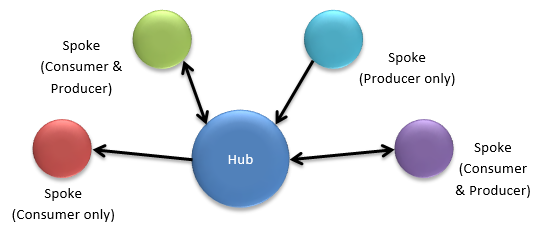
\includegraphics[scale=0.5]{res/hub-and-spoke}
\item \textbf{Source/Subscribers} is a sharing model where one organisation functions as the single source of information and sends that information to subscribers.\\
\centering
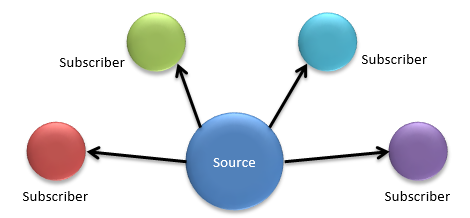
\includegraphics[scale=0.5]{res/source-subscriber}
\item \textbf{Peer to Peer}  is a sharing model where two or more organisations share information directly with one another. A Peer to Peer sharing model may be ad-hoc, where information exchange is not coordinated ahead of time and is done on an as-needed basis, may be well defined with legal agreements and established procedures, or somewhere in the middle.\\
\centering
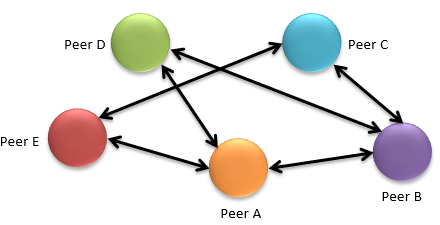
\includegraphics[scale=0.5]{res/peer-to-peer}
\end{itemize}


On the other hand, in the \gls{misp} project, they decided to support more attribute types and to have an easier model to use. Therefore, A. Dulaunoy and A. Iklody describe an alternative to \gls{stix}, the MISP core format, in the second version of the draft\cite{MispDraft} while still allowing to directly export data into the \gls{stix} format in the web interface. On the other hand, they are using the Hub and Spoke \gls{taxii} model for transportation as explained in the introduction.

\section{Contextualisation}
When I started the master thesis, my knowledge about threat information sharing was clearly none. I had to look up for articles and information where I was able to find some. I've finally chosen some articles and some points that I found interesting to share in order to understand the different steps I followed and the different ideas on which I thought about.\\
Also, I've spoken about \gls{misp} as it is the platform I'm interested in but there is an available really good awesome list \cite{AwesomeTreat} available where a collection of existing standards, tools and techniques are listed (Unfortunately I found it only at the end of the master thesis).\\
But in order to come back to \gls{misp}. The main advantages compared to the proprietary solutions are that:
\begin{itemize}
\item[$\bullet$] Transparency in term of code and of the contributor.
\item[$\bullet$] Quantity and diversity of connected entities
\item[$\bullet$] The price and the non-existence of entrance barriers\info{Any additional are welcome}
\end{itemize}

In the state of the art, I've also spoken about attack scenarios and cardinality of the intersection to evaluate the benefit of sharing before doing it. These kind of techniques are not yet implemented in \gls{misp} but could appear one day.\\

Back on the sharing problem have a dataset of malicious data, \gls{ioc}s, events coming from \gls{misp} and we want to share them in a privacy-preserving way and moreover, we want to get rid of this needed trust in sharing.
Computer specialists would be able to check on computers to discover infections, problems and moreover learn how to fix them thanks to previous analyses contained in \gls{misp}. The problem is that some information are confidential and we need to have some confidentiality concerns while sharing. \\


Then, it was really useful to see these existing techniques but it unfortunately does not mean that it could solve all of our problems. They had other purposes when designing their solutions and it can lead to some disadvantage in what we are attempting to do.\\
Sanitisation is a good example as it is really useful for the existing implementation but in this case, it would modify data up to make them unusable for everyone.\\
Other sharing strategy needs server always up which is not interesting either so we still need to find a way of sharing only if the user has really knowledge of the event and can share information on it as well, or is really infected by and need help that could be given by the information.\\


\section{Limitation: What could be expected from this work}

The goal of this master thesis is to generate rules representing IOCs and that can be shared without directly revealing information. We thus know that, as the information is given, an attacker can retrieve the information from it by bruteforcing the encrypted data. We therefore only can make it more difficult as we can up to try to make it unfeasible.\\
Unfortunately data like IPv4 are a problem by the number of possible values which is of 4 billions. This is feasible for the actual computer power to test every possible ones. This means that we need to make it really hard but it also makes it hard for a normal user to use it though. We thus already knows that we are going to need to find a trade off.

\chapter{Implementation Concepts}

Now that the subject seems clearer, there are a lot of different possibilities that could be explored. This chapter will be the opportunity to dwell on some of them in order to look for their strong points as well as their weaknesses.

\section{Bloom Filters}
Bloom filter is a space efficient probabilistic data structure  used to efficiently test the membership of specific values.\\
It has an enormous advantage which is to be able to test for membership without requiring to store the complete set of data. On the other hand, even if this data structure never forgets a member, it can falsely believe in the membership of a value even not related to it. The rate to which a data is wrongly recognised is called the False Positive rate and will be explored later on.\\
This small example of a small dataset of small data already shows the memory advantage: the data set of all the students' name and surname at Harvard. Taking the hypothesis that each name and surname has approximately 6 characters and that there are about 20 000 students. The dataset should use 20 000 * 6 * 2 * 8 (=1920 000) bits while a 1\% false positive bloom filter could be only around 20 000 * 10 bits which is already about 9 times smaller.\\

\subsection{Data Structure}
A bloom filter is a m bits array (fig. \ref{bloom-1}) with bits all set to 0 at the starting point. Besides that, there are also k independent hash functions. 

\begin{figure}[h!]
	\begin{center}
		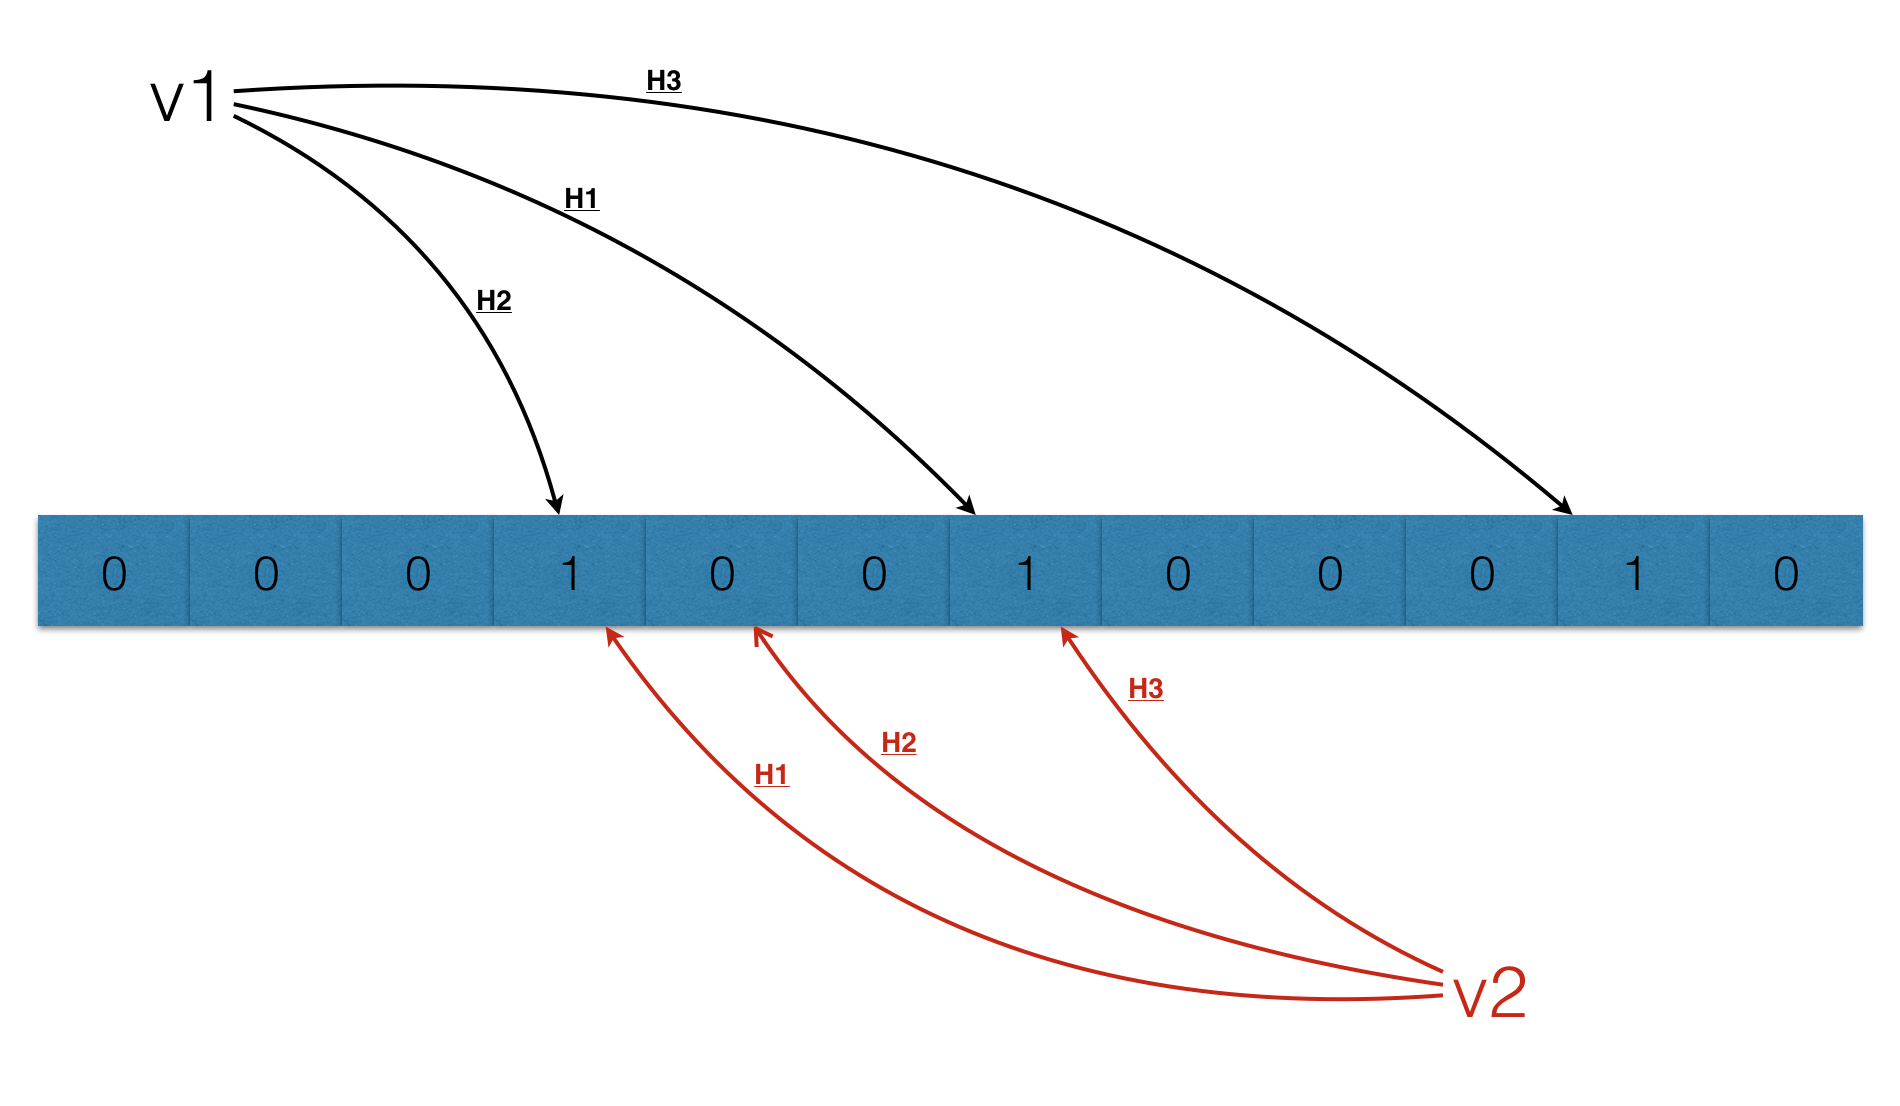
\includegraphics[scale=0.3]{res/bloom-1}
		\caption{Bloom Filter with m=12 and k=3}
		\label{bloom-1}
	\end{center}
\end{figure}

To add the value v1, each hash function gives a fingerprint of the value which is considered as an index in the array where the value needs to be set to 1. In the opposite, if we want to test a value for membership, we have to check all indexes given by the hash functions. As we can see on figure \ref{bloom-1}, v1 is in the set while v2 is not.

\subsection{False Positive Rate}

Bloom filter is a probabilistic data structure as when we are checking for a value, either the value is \textbf{not} in the set or is \textbf{perhaps} in the set. \\
In the latest case, this is due to false positive where all the k hash functions give indexes already set to 1 while the element should not be in the set.\\
An example can be seen on figure \ref{bloom-2} where v3 do not belong to the set.

\begin{figure}[h!]
	\begin{center}
		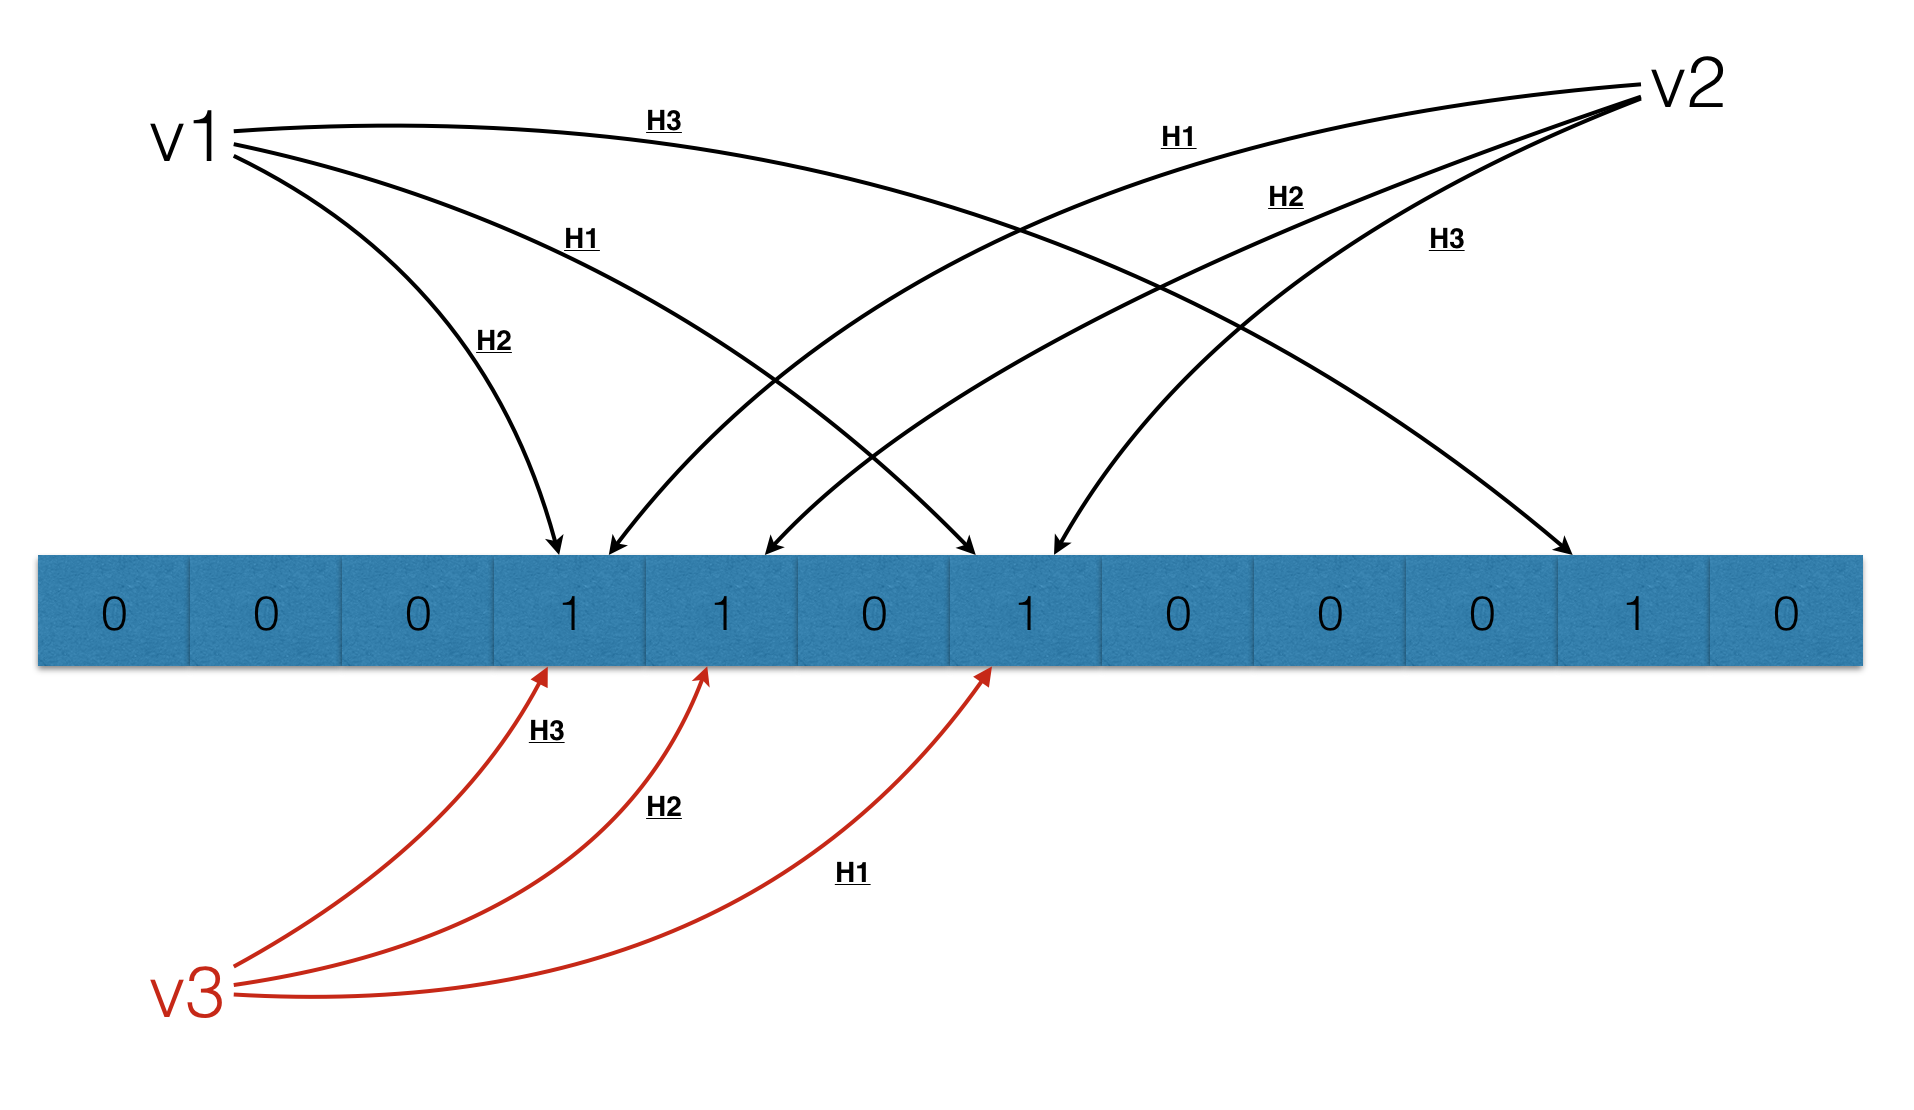
\includegraphics[scale=0.3]{res/bloom-2}
		\caption{False positive v3 in a bloom filter with m=12 and k=3}
		\label{bloom-2}
	\end{center}
\end{figure}

\subsection{Control the False Positive Rate}
If we check for a value in a bloom filter, at the end, we only know if it is not in the set or a probability to be in the set. Playing with this probability could be interesting for hiding some information and can be a really important feature for privacy and confidentiality.\\
This is why it could be useful to get more information on the false positive rate and how we could use it.\\

If n is the number of elements inside the data structure we can approximate\footnote{https://en.wikipedia.org/wiki/Bloom\_filter} the false positive rate by $(1-e^{\frac{-kn}{m}})^k$ but a more useful way is to define k in function of the willing rate for the false positive. In this case, we can notice that k is independent of the number of elements inside the set while on the opposite, it is m who needs to be changed in function of the number of values n:
$$m = - \frac{m\ \ln(p)}{\ln(2)^2}$$
$$k = - \frac{\ln(p)}{\ln(2)}$$
(These are approximations)

\subsection{Information Leaked by Bloom Filters}
It could seem useless but nevertheless, it could have huge impacts. If we create bloom filter and we ensure a false positive rate, with the size of the array (m), the number of hash functions (k) and the number of bits set to 1(X). An attacker could approximate the number of values in a bloom filter like shown by Swamidass et al. \cite{swamidass2007mathematical}:
$$n* = - \frac{m}{k} \ln\left[1 - \frac{X}{m}\right] $$

This does not bring a lot of information and the number of elements in the set is leaked as well in the final solution but it is important to have a knowledge of that while implementing a system based on those solutions.

\subsection{Is this a complete solution to the problem?}
It is not enough alone as we not only need to test element for membership but we also need to get back information on it.\\
But it is still an interesting solution and could have great benefits once twinned with a later explained implementation.

\section{Machine Learning}

Machine learning is \textbf{the} actual technology for security. A system that could evolve and learn by itself. No need for updates! \\
Early in April, "Beyond the blacklists: Detecting malicious \gls{url} through machine learning" showed at the Black Hat Asia conferences that it can work.\\
They focused on \gls{url} lexical features like the \gls{url} length, vocabulary, path, hostname, parameters, HTTP headers (in average, there are fewer fields with malicious connections) and they manage to get an 84\% detection rate on about 750K malicious \gls{url}s which is really promising.\\

Machine learning is thus a really promising tool in this domain but, the idea here would be to use it completely differently. We don't want it to continuously learn but we want an algorithm to learn a specific data set.\\
Then the control of false negative and positive would be done via overfitting.\\
In this particular case, overfitting is what is needed as we are not interested in inference but just in recognising the elements' membership.\\

This technique could be interesting to keep more control on the privacy and confidentiality, an attacker would learn even fewer things than with a bloom filter.\\
For the size, a model can also fit with less memory than remembering the whole set but will differ in each algorithm.\\
So the Base Concept Representation (BCR) of this technique on different example could bring a lot of information on the usability of this technique. But it could be difficult to tune and would have the same disadvantage as the bloom filter which is that it only decides membership and cannot give useful data back to the user. One last important thing to be aware is that some kind of models could leak information inside them for someone really understanding the system. (Ex clear decisions for a decision tree)\\

This technique has the advantage of bringing more data protection due to the false negative rate but it also looses an important characteristic as it could be bad to know an attack \gls{ioc}s but does not detect it because of that rate.

\section{Secure Multi-Party Computation}
Each organisation possesses its \gls{ioc} database and is not ready to share all their information. But, once again, if it could help another organisation to solve its problem, they agree on sharing only these information.\\
That is where Secure Multi-Party Computation could play a role as there are techniques to find the intersections of 2 datasets. This is also called private matching \cite{agrawal2003information, li2005private}.\\

This technique has only a big disadvantage which is heavy computations on both sides. But still, it could be very useful to share information between \gls{misp} instances.

\section{Proof of Work Database}
This idea is to slow down brute force attack thanks to proof of work. Even if this idea is one step closer to the final implementation, it is still different by the need of a server to communicate with for each request.\\

Here, we want to keep a database, we don't want any false positive nor false negative. But by doing that, we make our database available to brute force attacks.\\
We just need to add a new wall of time-consuming computations between the user and the dataset for the requests.\\

A possible implementation could be with a random key chosen by the database server. This key could be regenerated with a small period and also every thousand\footnote{This number can be modified with the user will} requests.\\
On the other hand, the client should brute force this small key each time it has changed. This slows down brute force attacks while still be useful for a user that is doing less than one thousand requests to test its systems.

For example, a possible request message for an \gls{ip} could be : hash(IP)||hash(IP||key)\\

The idea is interesting even if it is still not bullet proof against brute force attack. It also need a server to respond at each request.

\section{Conclusion}
I've explained some basic ideas that could lead to different implementations, a lot of work are done especially on private multi-party matching that could lead to the best option if requests are rare or, for example, if it is used to periodically compare and synchronise data related to the same events between \gls{misp} instances.\\
Nearly every solution still needs a server that we would like to get rid of (After the data had been generated) and for that, a machine learning model or bloom filters are the right track but there is still a lack as we do not get back information. That is why the final implemented solution will find something similar to proof of work  to slow down the attack and the bloom filter to increase the system speed.



\chapter{Implementation}
I've explained ideas in the previous chapter, some of these could be implemented. But a nice article \cite{van2016private} was published in the few first months of my work and they had found a technique that could also work here as their goal was a similar one: allow parties to share information without the need to immediately reveal private information.\\
Their implementation was for bro, here I will make an implementation working with \gls{misp} and improve its matching properties and the modularity of the code. \\
By modularity, I mean that I want to be able to add "cryptographic modules" in order to test different techniques with the same code.\\
In this chapter, I will first explain their article, then the modifications and improvements I've made.\\

\section{Private Sharing of IOCs and Sightings \cite{van2016private}}
\label{sec:articlePrivate}
This paper considers a cryptographic approach to hide the details of an indicator of compromise. They consider two different phases, sharing these \gls{ioc}s and privately reporting the sightings of \gls{ioc}s.\\

Reporting the sightings is important for monitoring the events and attributes in \gls{misp}.\\ 
Moreover, \gls{misp} is now able to remember a sightings number per attribute but their technique seems difficult to implement in \gls{misp} for a standard subscriber as we should go through each attribute for each instance and each reporter while being online periodically (not practical at all). I've got some other ideas but I finally only focused myself on the sharing part as I would have not enough time.\\ 
But still, It could be the most important and really useful further work to do.\\

They also started by warning the reader that using these cryptographic function is better than not using them at all but it is not a miracle technique as it is theoretically impossible to hide the \gls{ioc}’s content in the used context (Subscribers receive the data to check on theirs systems).\\
Additionally, it has a performance cost but in my beliefs, it is well worth it.\\ Their implementation is in the source-subscriber \gls{taxii} sharing model but it can nevertheless fit with our model.\\
First, they define an \gls{ioc} as propositional formula where the propositional variables are defined over features or observables like Internet Protocol (\gls{ip}) or fingerprints of malicious programs (but it could be any IOCs contained in \gls{misp}). They also claim that every \gls{ioc} can be expressed in the Disjunction Normal Form (DNF) without any negation (e.g. destIP= 198.51.100.43 $\land$ destPort = 80).\\
Hereandafter the values of the rules generated are considered as the concatenation of all values of the \gls{ioc}s that are linked together: \gls{ipv4}$||$port\_number. It has two advantages, the first is to represent all linked values directly together and then, increasing the size and the number of elements hashed increases the difficulty for an attacker to perform a bruteforce attack or to precompute all possible hashes.\\

\begin{figure}[h!]
\begin{center}
	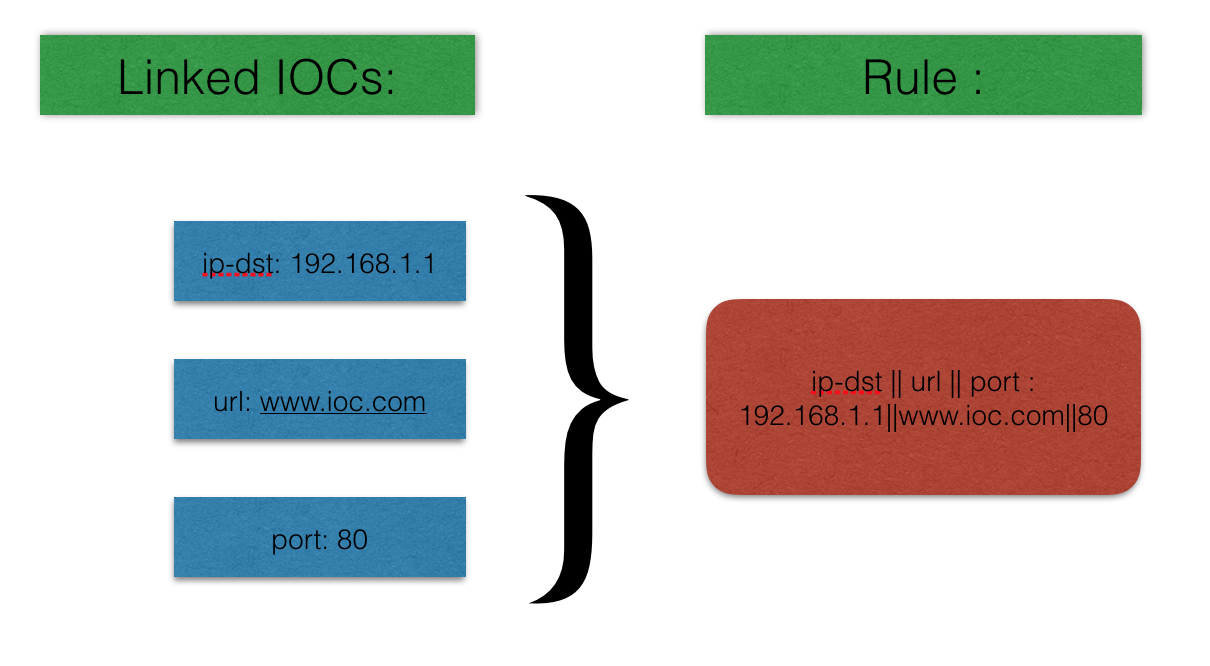
\includegraphics[scale=0.5]{res/ioc-rules}
	\caption{IOCs transformed into a rule}
	\label{IOC-To-Rule}
\end{center}
\end{figure}
\improvement[inline]{Not Combined IOCs But RELATED}

Rules, as created, can be directly checked on computers but they do not fit with our model yet as every value are still in clear. To solve this problem, they decided to hash the values concatenation while still keeping the structure (e.g. ip-dst||port) in clear.\\
The structure is what makes it still usable as it says the user which are the type of values they need to try against the rule.\\
The only additional computation is that the user needs to hash his values each time he tried to match the rule.\\
In this way, we are still really close to the hashstore previously explained but with the advantage of being able to individually store and share rules. We still lack some protections since every individual variable can only take a limited set and we still do not get back information while there is a match.\\
For solving that, they are using a non-secret salt value chosen at random for \textbf{each} rule (\gls{ioc}). Besides that, the attack time can be increased as well thanks to the cryptographic hash function used. The second part is really affecting the honest subscriber performance as well but is needed to slow down enough an attack for small data.\\

They didn't stop there, considering all these ideas, they have added the possibility to include a \gls{coa} message with each rule. This is the real advantage compared to other techniques. The output is precise, there are neither false positive nor false negative and additionally, a match can give information to the honest user.\\ To do so, instead of hashing the combined values, they use it as the input of a \gls{kdf} that generates a key used for encrypting a message.\\
Thus this new type of rule, instead of just obfuscating the data, contains the type of value (as before), the salt used for the rule and the encrypted message.\\


\begin{figure}[h!]
\begin{center}
	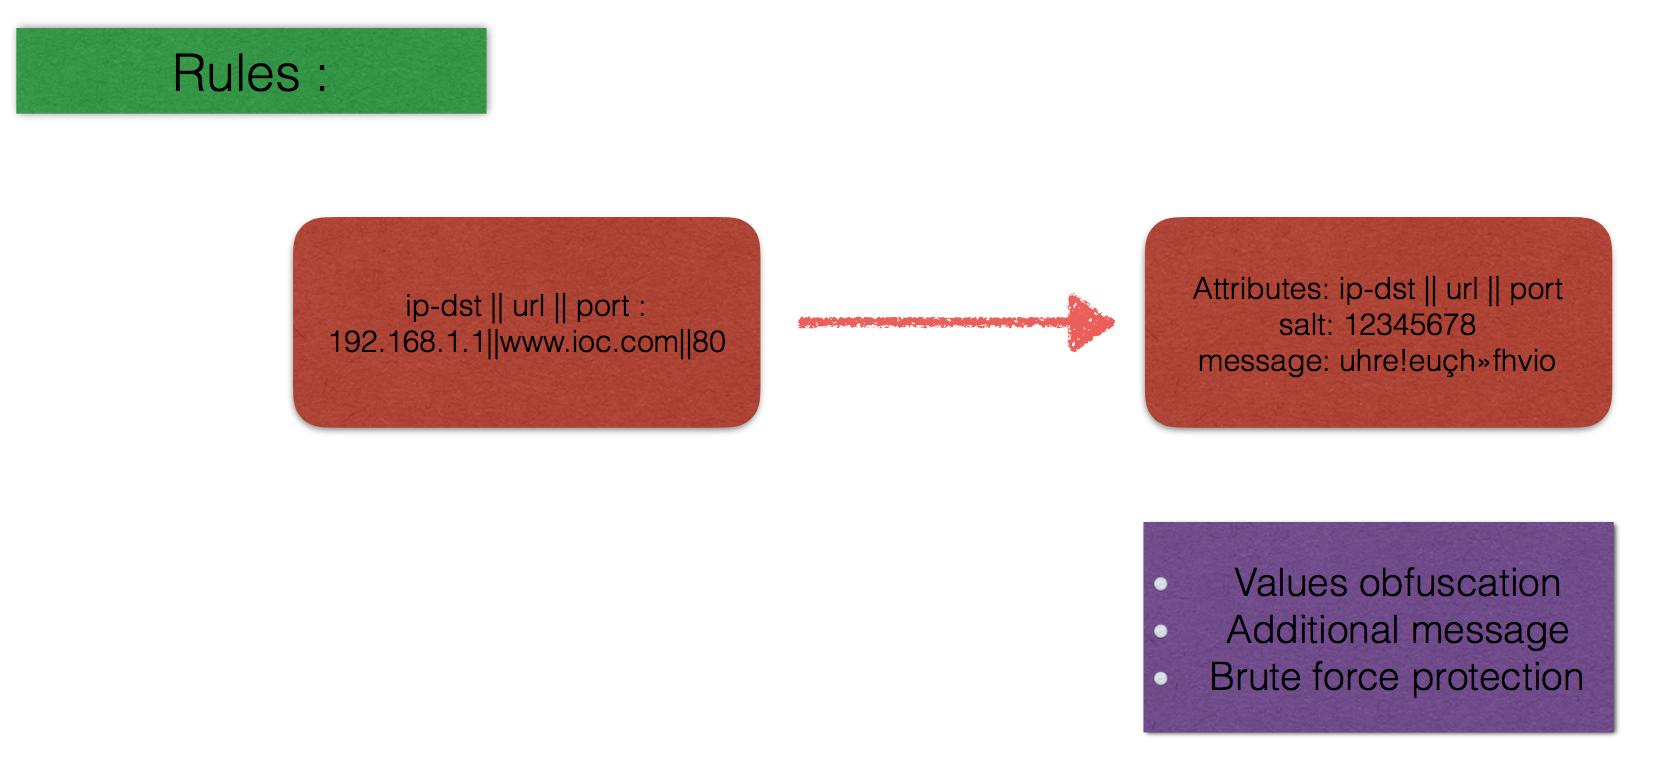
\includegraphics[scale=0.5]{res/obfuscation-rule}
	\caption{New format for the rules}
	\label{Obfuscation-Rule}
\end{center}
\end{figure}


This pseudo code shows how to generate a rule from the \gls{ioc}s:

\begin{center}
\begin{boxedverbatim}
Function createRule(AttributeTypes, values, message, Token):
        pass = '||'.join(values)
        salt = GenSalt()
        key = kdf(token + salt + pass)
        message = 16 * '\x00' + message
        encr_message = encrypt(message, key)
        return dictionary(attributes=AttributeTypes, 
                            salt=salt,
                            ciphertext=encr_message)
\end{boxedverbatim}
\end{center}

Then, this pseudo code explains how to check values against one rule:
\begin{center}
\begin{boxedverbatim}
Function matchRule(dictianary(type -> value), rule, token):
        pass = '||'.join(values in rule.attributes)
        key = kdf(token + rule.salt + pass)
        if (decipher_16first_bytes(rule.message, key) = 16 * '\x00'):
                return decipher(rule.message, key)
        else
                return notMatched
\end{boxedverbatim}
\end{center}


Trust is one of the major problems in information sharing and is discussed in all standards, guides and articles. Here they have an attempt of solution that could really work. As a user cannot normally decrypt the complete rules data set, if for each generated rule, we add a source identifier in the \gls{kdf}. This results in the ability to track the origin of a leak. \\
Even if it is a small addition, I'm intimately convinced that it could help organisations to decide to share more confidential data as they could turn themselves against the leakage source in case of problems which could limit the cost damage as well as the reputation damage. Moreover, in \gls{misp} there is also a user identifier that could be used and which is called a Token.\\

In their implementation, they are using both \gls{hmac} and \gls{pbkdf2} for the key derivation function. I had the opportunity to exchange emails with the main author of the paper that prefers the \gls{hmac} algorithm as it is designed to give a pseudo random key in just a single iteration and that it has been deeply analysed \cite{cryptoeprint}. While \gls{pbkdf2} is generating random keys that become more secure as the number of iterations increases. Moreover, the behaviour has not been described (to the best of our knowledge) in academic paper even if there is a \gls{nist} recommendation on its usage.\\
They also used an \gls{aes} encryption scheme to encrypt the CAO message.\\

Their proof of concept code is available on their repository, \url{https://github.com/CRIPTIM/private-IOC-sharing}. 


\section{My Implementation}
The article of Tim van de Kamp et al. gave me the starting point I needed as the code was available and under the MIT license. I've thus created two basic scripts starting from theirs where I've written it back to fit with \gls{misp}. At first, I've kept exactly the same scheme as they are.\\
The first step was to retrieve data from \gls{misp}, either from the web \gls{api}, by a direct connection towards the MySQL database or directly via \gls{csv} files.\\
Then I've improved the code with different new functionalities and realised that, on the contrary of all university projects we had, the project needed to often be completely refactored to allow additional features and to keep it simple for an external user to understand how it works. I will thus go through theses different implementation parts in the next few sections.\\

\subsection{Get data from MISP}
To create the rules with the encrypted messages, we first need to get a subset of \gls{ioc}s contained in \gls{misp} that are destined to \gls{ids}. \\
For doing so, there are tree possibilities, the first one is working with the \gls{misp} web\gls{api} while the second one is directly connected to the MySQL database. \\
The third one that directly reads from a \gls{csv} file had been added to be able to select what should be shared and for a testing purpose.\\
The recommended mode will be with the web \gls{api}, but as rules will be generated directly on the server, it could be more efficient to use directly the MySQL connection.\\

For making automated request on \gls{misp}, they have implemented a python library called PyMISP. The first idea was to use it but it was finally not interesting to import the whole library only to make one request. That is why, I've changed the system by making myself the requests to the automation \gls{api} by using the requests python library and the \gls{misp} token referenced in the configuration file.\\

The virtual machine has been a great utility to understand how it is working, and especially how the database is structured. I've also added an additional check like verifying that the email address specified is the one related to the token when the MySQL connection is used.

\subsection{Parsing logs}
The idea was to test the system with log files as I did with the hashstore. First I tried to reuse the parser I've created but I tried to go too deep in the analyse and it has bad performances as well as a lot of particular cases that were not working.\\
I thus changed my mind and used logstash and redis to store the parsed log. \\
It also has the big advantage to be modular and only a new configuration file is needed to parse any other type of log files.\\
Besides that, I'm storing the data inside a redis queue and polling on it in the script for trying to match a rule. \\

\subsection{Multiprocessing}
When there are a lot of logs, look at them one by one takes too much time, but we can test simultaneously more than one log line at the same time by creating processes.\\
Also it is important to point out that I've started this by trying to use threads but, as I'm using the cpython interpreter, it is impossible to have two programs running simultaneously due to the Global Interpreter Lock (GIL). That is why, I finally chose to create a pool of processes instead.

\subsection{I/O and Rule Size Optimization}
In the implementation of Tim van de Kamp et al., for each rule, they created a file to store the rule. \\
It works for a proof of concept but it is a really bad idea in UNIX systems. Each file has a minimum size of 4k. Already with 6300 events each one possessing 153 attributes in average, it is easy to see the problem coming. Moreover, the I/O functions were really slowing down the system. \\
These problems were easy to solve by creating a complete \gls{csv} file for all rules. But was still not a complete solution because it would mean that we should load everything in memory even if we don't use everything. That is why I finally chose to have one \gls{csv} file per type of \gls{ioc}s. For example, the system creates files url.csv, ip-dst.csv ...

\subsection{\gls{csv} or \gls{tsv}?}
This is a really small modification but makes files more readable and avoid existing coma in the data to make the parsing not working.\\
Therefore, I have chosen the tabulation instead of the coma as an element separator in the rules.

\subsection{\gls{url} Normalisation}
The goal of the system is looking for matches in \gls{misp} data. But off course, if an event has for Uniform Resource Locator (\gls{url}) www.ioc.com I would like http://www.ioc.com, http://www.ioc.com/, http://www.ioc.com:80/, ... to match as well.\\
I first dug a little into \gls{url} normalisation like the standards and techniques already used in practice. I've realised that normalisations are difficult as, in the standards, they want \gls{url} to always work after, and really be the same. For example http://www.ioc.com is not https://www.ioc.com while in matching, I absolutely don't care and I would like to both trigger an alert.\\
Besides that, there are standards on \gls{url} normalisation [\gls{rfc} 3986] that contains either normalisations that preserve or usually preserve the semantic of the \gls{url} but none that does not preserve it.\\
Standards are thus focus on keeping the number of false positive near to 0 but it has for impact to miss a lot of real positive and we cannot afford that.\\
I've thus found this paper \cite{lee2005url} which was focus on \gls{url} normalization and that goes beyond standards normalization steps like case sensitivity in the path, the last slash symbol at the end of the path and the designation of the default page (index.html, ...).\\
Besides that, a great summary of all these standardizations steps is available on wikipedia \cite{wikiNormalizationURL}.\\
In the implementation, I've used the python library url\_normalize:
\begin{itemize}
\item[•] Take care of IDN domains.
\item[•] Always provide the URI scheme in lowercase characters.
\item[•] Always provide the host, if any, in lowercase characters.
\item[•] Only perform percent-encoding where it is essential.
\item[•] Always use uppercase A-through-F characters when percent-encoding.
\item[•] Prevent dot-segments appearing in non-relative URI paths.
\item[•] For schemes that define a default authority, use an empty authority if the default is desired.
\item[•] For schemes that define an empty path to be equivalent to a path of "/", use "/".
\item[•] For schemes that define a port, use an empty port if the default is desired
\item[•] All portions of the URI must be utf-8 encoded NFC from Unicode strings
\end{itemize}

I thus added some additional steps like:
\begin{itemize}
\item Removing directory index : {default.asp, index.html, index.php, index.shtml, index.jsp, default.asp}.
\item Remove the fragment (\#...) which is never seen by the server.
\item Removing the protocol {http://, https://}.
\item Removing  “www” as the first domain label.
\item Removing the "?" when the query is empty.
\end{itemize}

\subsection{\gls{ip} Normalisation}
Like for the \gls{url} some \gls{ip}s can be expressed differently due to shortcuts. For example, the \gls{ipv6} address 2001:0db8:0000:85a3:0000:0000:ac1f:8001 is equivalent to this \gls{ipv6} address 2001:db8:0:85a3:0:0:ac1f:8001 as well as 2001:db8:0:85a3::ac1f:8001.\\
Moreover, some attributes specify an \gls{ipv4} range instead of an \gls{ipv4}. This also need to be handled in a proper way.\\

To solve these problems, I'm using a simple library called ipaddress with two specific functions, ip\_network for handling the ranges and ip\_address to handle standard \gls{ip}s.\\
The last function creates an object which is either an \gls{ipv4} or \gls{ipv6} instance. For the \gls{ipv6} address 2001:0db8:0000:85a3:0000:0000:ac1f:8001, it would return IPv6Address('2001:db8:0:85a3::ac1f:8001'). Then a simple str function allows to get back the normalised value.\\
Also, this function raises  an error when there is a problem with one \gls{ip}, in this case, I simply add them without any changes and print the problematic value.\\
This is actually how I discovered the \gls{ip} ranges and also that some \gls{ip}s are not interesting as a rule as they have the host bit set to one.\\

For the \gls{ip} ranges, there are two possibilities to handle them, either we create ranges and it matches only if the user try the range (meaning that when trying to match an \gls{ip} we also need to try to match the different possible ranges) or, we can accept only ranges '/x' where x >23 and for these cases, create the 256 (or less) possible rules.
The second could be really inefficient due to the high number of generated rules. While the second one would approximately double the time for each match while only considering the range /24 and could not accept the ranges between 24 and 32.\improvement[inline]{CHOOSE ONE SOLUTION AND IMPLEMENT IT}


\subsection{\gls{pbkdf2}}
While I was adding features, it becomes more and more difficult to allow all these possible choices, I've thus started by limiting the key derivation function (\gls{kdf}) choice to \gls{pbkdf2} which is not the author advised one but allow to parametrise the difficulty for an attacker to brute force some small data.\\
But in the opposite we cannot have a small number iteration if we want the key to look random. Which is finally the intended behaviour as we want to slow down bruteforce attacks.\\
Then, I've implemented an other \gls{kdf} following the same scheme as with \gls{pbkdf2} called Bcrypt which is explained in \ref{sec:BcryptExp}

\subsection{Library: Pycrypto towards Cryptography}
While discussing with Tim van de Kamp by email, he said that if he had to start over, he would choose the cryptography library \footnote{https://cryptography.io/en/latest/} instead of pycrypto because it seems to be a more professional implementation.\\
I thus have made some research on it. There are some discussion about it but \url{libhunt.com} gives this table \ref{cryptoLibraries} where we can see that even if pycrypto seems better written, the cryptography library is more up to date and still with a lot of activities.\\
Besides that, I found the library well defined and really easy to use that is why, I've chosen to refactor the code with this particular library instead.


\begin{table}[h!]
\centering
\caption{Cryptography Libraries Comparison}
\label{cryptoLibraries}
\begin{tabular}{|l|c|c|}
\hline
                                                                  & \multicolumn{1}{l|}{{ \textbf{PyCrypto}}} & \multicolumn{1}{l|}{{ \textbf{Cryptography}}}                                              \\ \hline
Popularity                                                        & 7.2                                          & \textbf{7.3}                                                                                  \\ \hline
Activity                                                          & 0.0                                          & \textbf{9.0}                                                                                  \\ \hline
Stars                                                             & 1 345                                        & \textbf{1 431}                                                                                \\ \hline
Watchers                                                          & \textbf{103}                                 & 86                                                                                            \\ \hline
Last Commit                                                       & about 3 years ago                            & \textbf{\begin{tabular}[c]{@{}c@{}}7 hours before checking\\ on the 13 April 17\end{tabular}} \\ \hline
\begin{tabular}[c]{@{}l@{}}Code Quality\\ (L1 to L5)\end{tabular} & \textbf{L4}                                  & L2                                                                                            \\ \hline
\end{tabular}
\end{table}


\subsection{Structure Improvement}
The code was becoming less and less clear to understand and as I wanted it to be modular for the cryptographic system used. I've decided to completely re factor the code.\\
The used structure is now as following:
\begin{itemize}
\item src: Source code.
\item conf: Configuration files.
\item res: All downloaded useful resources like the \gls{csv} downloaded from \gls{misp}.
\item rules: Rules generated.
\end{itemize}

Inside src, there is also a crypto subdirectory in which are located all cryptographic functions in the different possible modules implemented.

\subsection{Top Configuration File}
Instead of having a lot of configuration files as when I started, I've gathered them back in one general file where we only have to fill in what will be used.\\
The configuration file is divided into categories and is read thanks to the configparser python library.

\subsection{The Encrypted Message}
In the original paper, the authors where using the Course Of Action (\gls{coa}) for the message. This is really useful to automatically react as soon as possible, but in our case we are mostly interest in protecting data as well as analysing the incident.\\
Therefore, my choice was to use a message to allow the user to retrieve the attributes and events on \gls{misp} and fetch the needed information. This has two advantages, the first one is to only allows to know that an element is known by \textbf{someone} using \gls{misp} and nothing more. This is really important for the privacy. Then, in order to get back information the user needs to connect to \gls{misp} where all authorisations are checked by the standard system.\\

Another point is that another advantage of this system is to be able to mix rules from different \gls{misp} instances. But for that, we need to be able to identify the different instances thanks to a universal unique identifier. After discussing it with CIRCL, It will normally be soon implemented.\\

Besides that, not every user needs the same message, so the message content can be modified with the top configuration file but in general at least the \gls{uuid} is needed to referenced uniquely the element.\\
The argument 'rules->message' is therefore associated with the attributes (separated by a space) contained by \gls{misp} attributes like : "uuid event\_id date".

\subsection{Add a rule}
After having created the \gls{misp} rules, if we want to add new ones, we can do it thanks to the addIOC script.\\
Then we can choose to specify the rule directly inside the terminal or via a \gls{csv} file located in the 'res' folder.\\
This needs to be used carefully as no verifications are made on the added rules. Checking every new \gls{ioc} if it already exists would have been really too time consuming.\\
On the other hand, unfortunately, bloom filters need to be completely regenerated for adding new rules.

\subsection{Update Rules}
After all that, making rules hard to bruteforce, makes it harder to generate as well. This is why we need the capability of updating the rules with the recent \gls{ioc}s.\\
This kind of implementation is only useful when the rules are generated via the \gls{misp} web \gls{api}. Therefore, the update implementation works only in this case.\\
First, a new metadata file is generated in the 'res' folder and keeps track of the last \gls{ioc}s date. Then via the addIOC script with a '--update' argument, it gets the new \gls{misp} attributes thanks to a specific web request, saves it in an \gls{csv} file called update<number of the update>.csv.
The \gls{csv} events are then transformed into rules and added to existing ones before finally updating the metadata file with the new latest date.

\section{Chosen Cryptographic Systems}
The idea of the generalisation was to add modules for handling the way data are stored/encrypted, we can use completely different cryptographic systems later called modules. In this section, I will discuss my implementation choices for each implemented schemes.

\subsection{\gls{pbkdf2}}
This is the basic system for which all the structure had been optimised and had been thought for. In this section, I will thus briefly introduce these two sequence diagrams to help the understanding of the system:
\begin{figure}[h!]
\begin{center}
   \begin{minipage}[c]{.46\linewidth}
      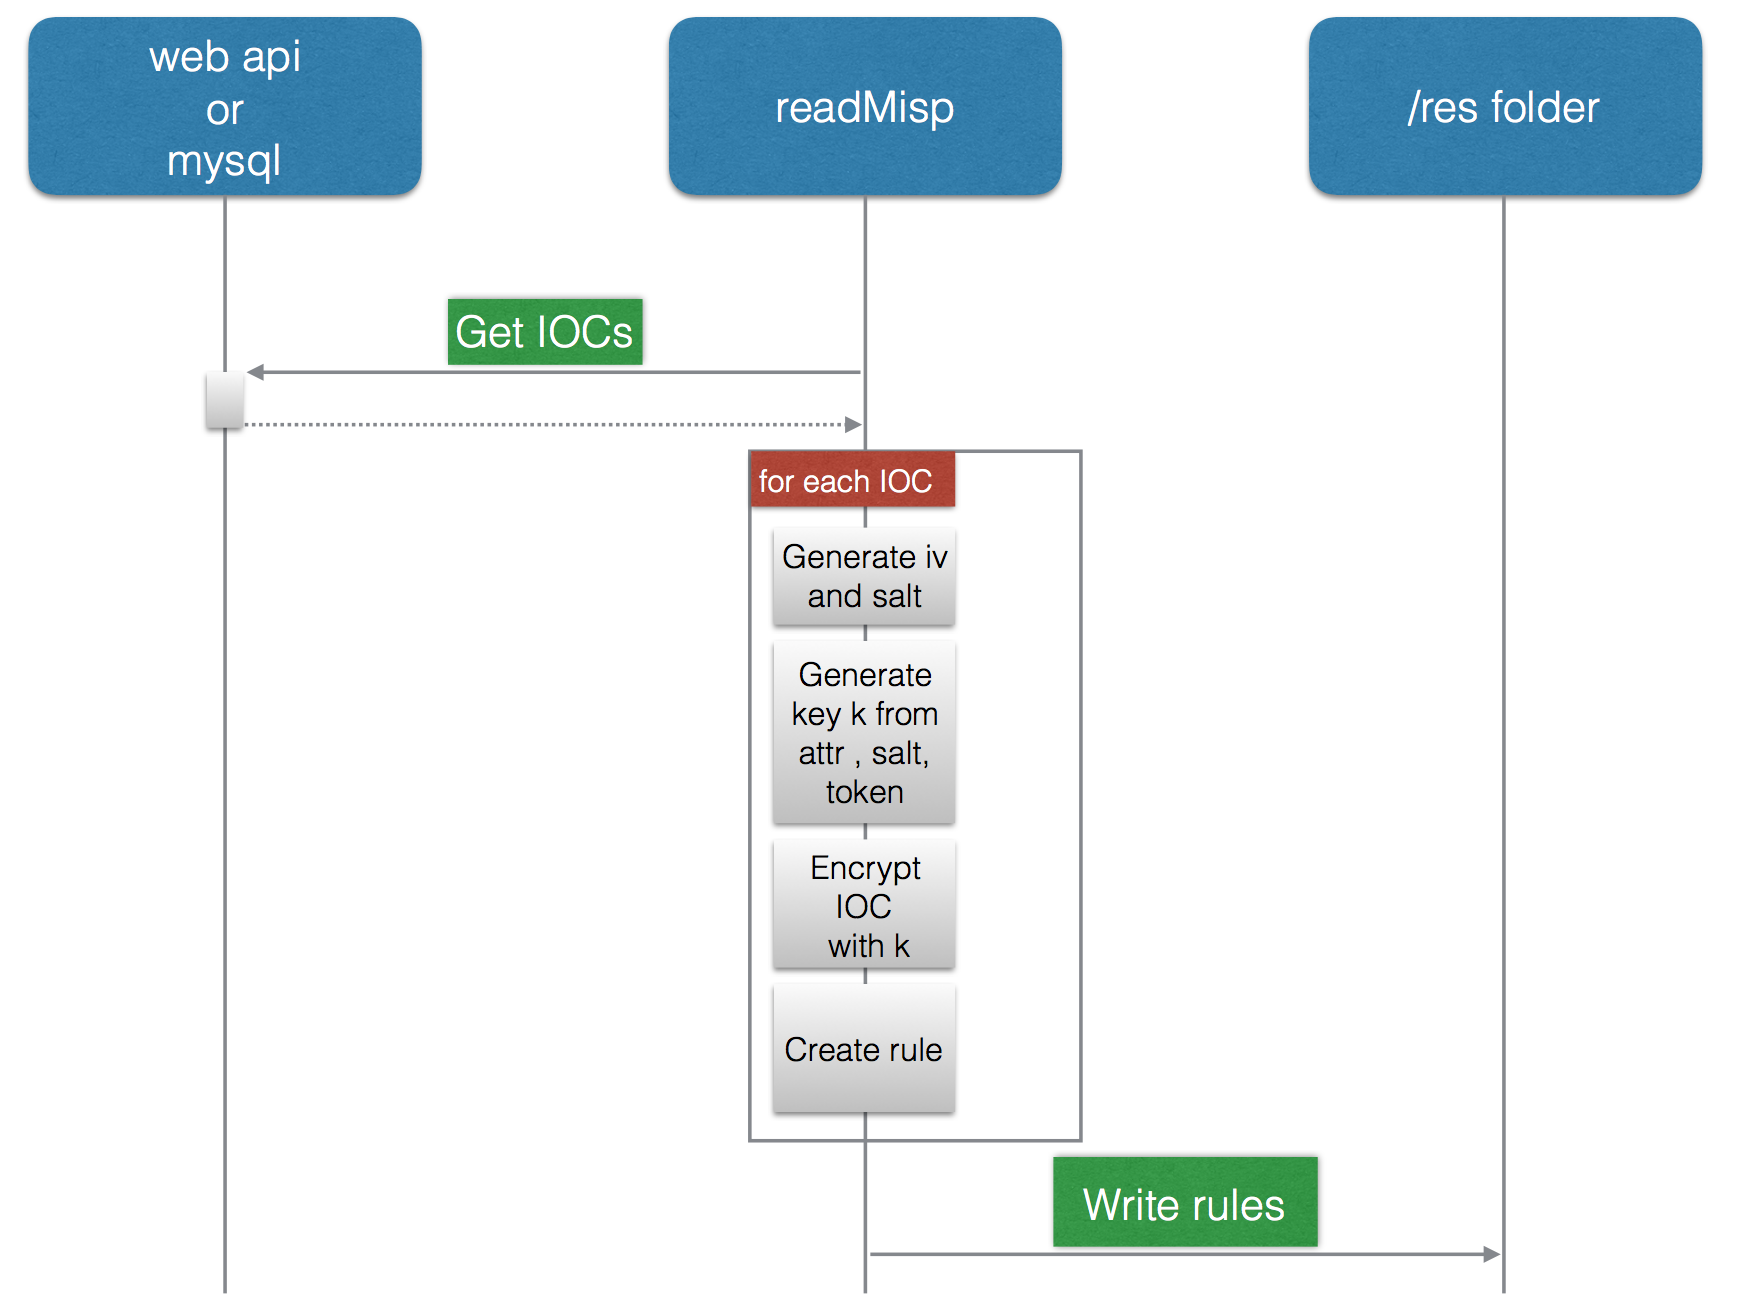
\includegraphics[scale=0.25]{res/seqDiagramRead}
   \end{minipage} \hfill
   \begin{minipage}[c]{.46\linewidth}
      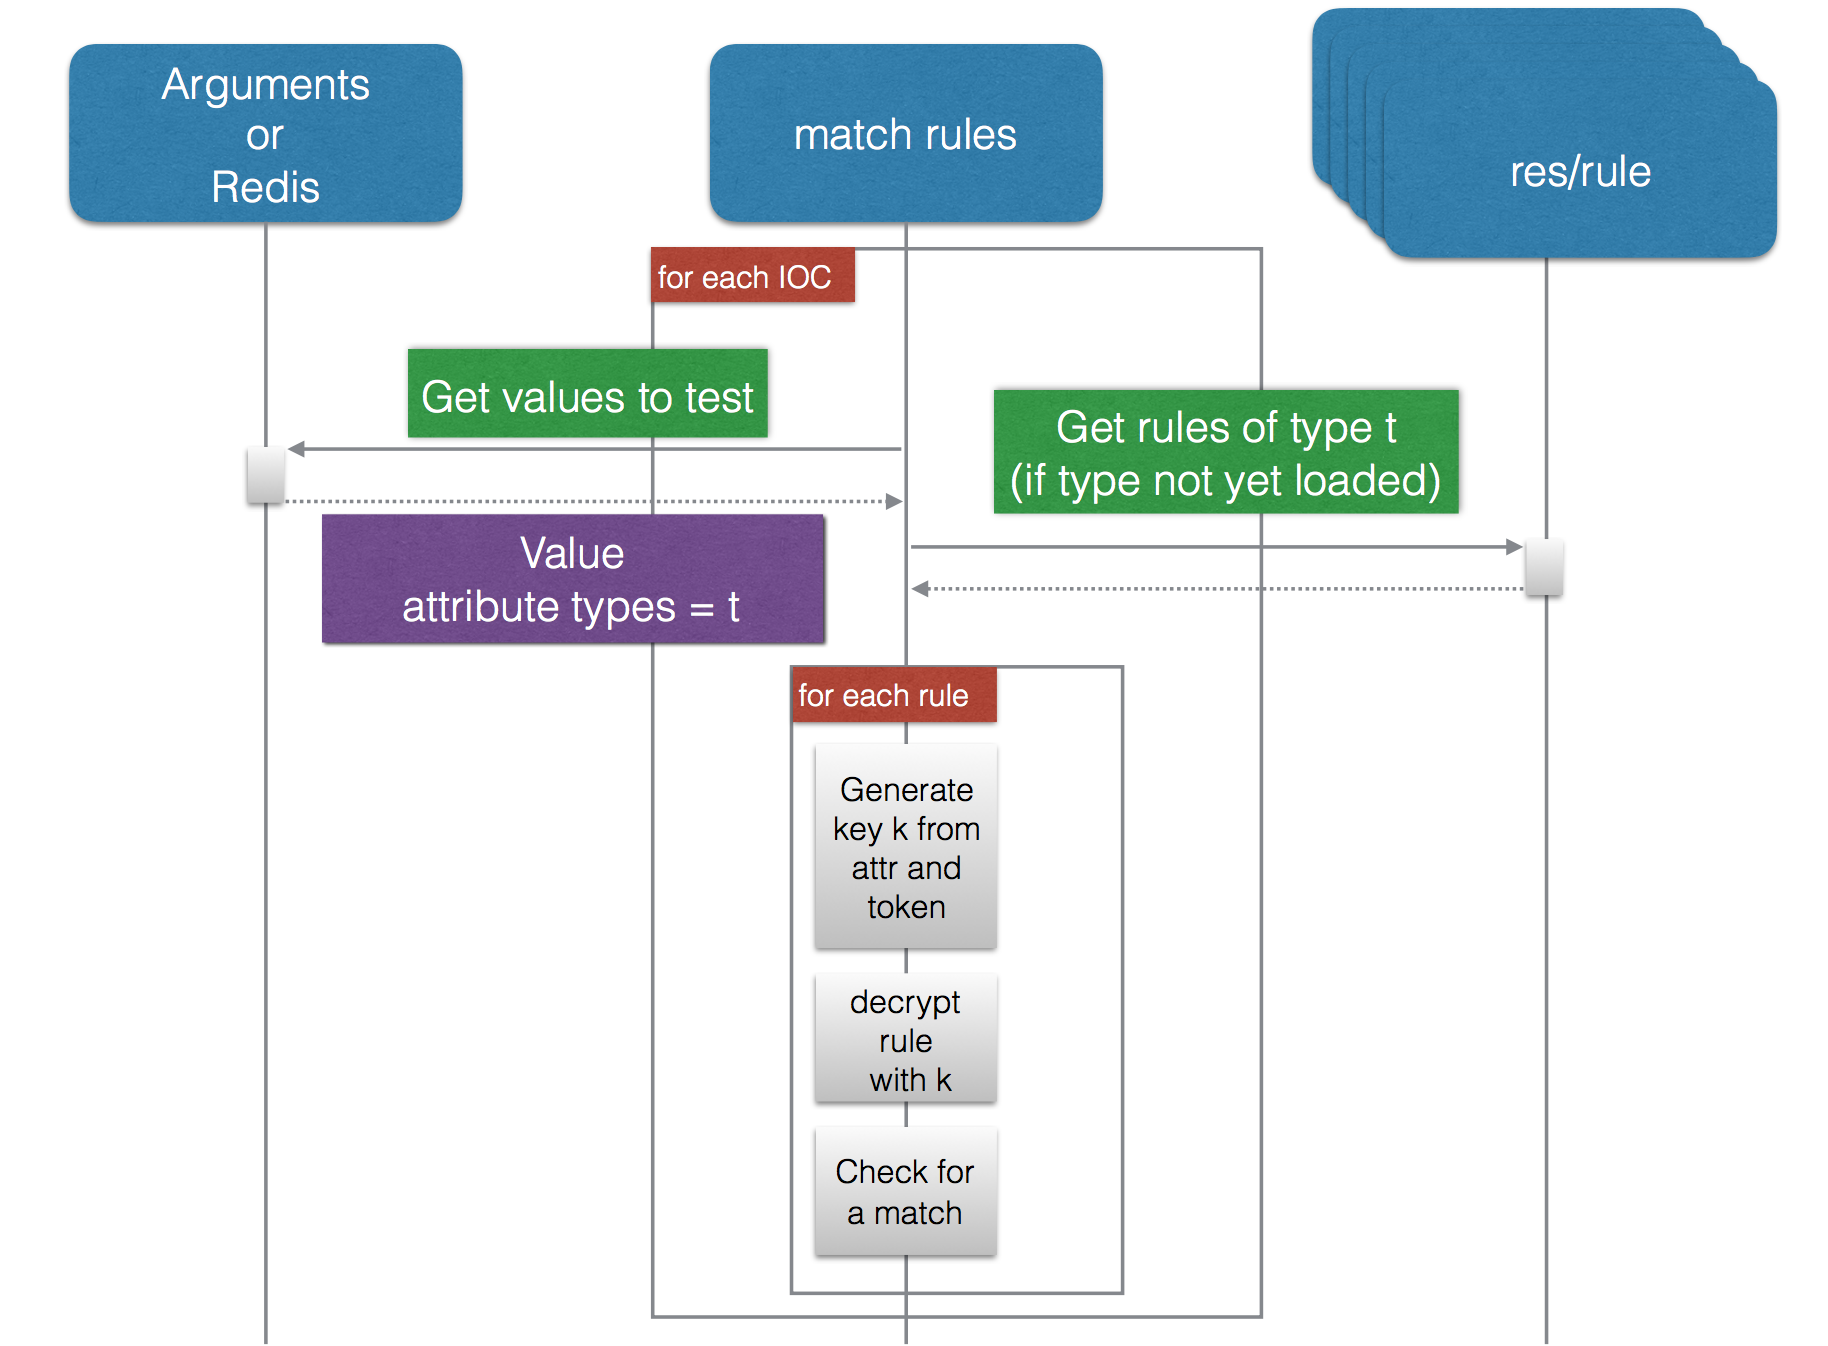
\includegraphics[scale=0.25]{res/seqDiagramMatch}
   \end{minipage}
\end{center}
\end{figure}

For the cryptographic system, there is also a small difference in the rules that allow a really faster matching.\\
Instead of directly encrypting the whole message, I've decided to divide it into two parts (easy to do with the cryptography library). The first is the ciphertext-check and the other one is the ciphertext. The ciphertext-check is simply the first block of the encrypted message. It is used only for matching, decrypt it must result in only zeros if there is a match. (cfr. \ref{sec:articlePrivate})\\

For this algorithm, the user must choose an important meta parameter that will determine the "security level". This meta parameter is the number of iterations for the key derivation functions.\\
In 2000, the [\gls{rfc}2898] advised 1000 iterations for password storing. In 2015, OWASP password storage cheat sheet \cite{van2015password} advised about 10 000 iterations while \gls{nist} recommends in the appendix A.2.2 of its guide \cite{turan2010nist} to use as many iterations as it is possible with the needed performances.\\

Some additional analyses can be made on the ability to sustain an attack, the article made by the CryptoSense\footnote{\url{https://cryptosense.com/parameter-choice-for-pbkdf2/}} website is really well documented.\\
They have analysed previous work and have done some estimation for 2015. Their approximation is more a guess than anything else and I wouldn't dare to try their approximation for 2017 but I will nevertheless show their results to get a rough idea of what could be the time to crack a password from a key generated with \gls{pbkdf2} (\gls{aes} + SHA-1):\\
\begin{table}[h!]
\centering
\caption{Cryptosense table}
\label{Cryptosense-table}
\begin{tabular}{|c|c|c|c|}
\hline
Password Complexity & Estimated Entropy (bits) & 1 000 Iterations & 10 000 iterations \\ \hline
Comprehensive8 & 33 & 4h46 & 47h \\ \hline
8 random lowercase letters & 37 & 12h & 5 days \\ \hline
8 random letters & 45 & 123 days & 3 years 5 months \\ \hline
\begin{tabular}[c]{@{}c@{}}8 letters + numbers + punctuation \\ OR \\ 4 random Diceware words\end{tabular} & 52 & 325 years & 3250 years \\ \hline
\end{tabular}
\end{table}

Finally, here is a simple example of a rule generated with this system. This \gls{ioc} is ioc.com of type test \ref{Example-rule-pbkdf2}:
% Please add the following required packages to your document preamble:
% \usepackage[normalem]{ulem}
% \useunder{\uline}{\ul}{}
\begin{table}[]
\centering
\caption{Example of a rule}
\label{Example-rule-pbkdf2}
\begin{tabular}{cc}
{\textbf{}}  & {\textbf{rule}}                          \\
salt             & jiGxB1CdO43YiPk5NUIbcQY0tYlQltKME1YVLgKKvRI= \\
attributes       & test                                         \\
nonce            & IzizTKP6fVsWnidzEx4Pkg==                     \\
ciphertext-check & SxzWSDR3nA4h5HwdTg3WJA==                     \\
ciphertext       & RQMQ0a7dxJuFxhZDdLuCp72CWaT0wzn4+w==        
\end{tabular}
\end{table}

\subsection{Bcrypt}
\label{sec:BcryptExp}
This implementation is similar as my implementation with \gls{pbkdf2}. Bcrypt is a password hash function based on the Blowfish cipher, as \gls{pbkdf2}, It also incorporates salts to be protected against rainbow table attacks (TMTO).\\
It has also the advantage of being more configurable and is more efficient against GPU attacks. It also seems better to use but the \gls{nist} recommendations are still about \gls{pbkdf2}.\\

The problem with this algorithm is that it only considers the 72 firsts characters of the password for the key generation. It can seem a lot but even this \gls{url} \url{https://translate.google.com/#fr/en/72\%20caract\%C3\%A8re\%2C\%20ce\%20n'est\%20pas\%20beaucoup} is 88 characters long. This means that if we add the token at the end (like in \gls{pbkdf2}) it will not be included. On the other side, if we first put the token before the data, an attacker would know that the 40 firsts characters will always be the same and moreover, there would be only 32 characters left for the data which is not enough.\\
As the goal was that the whole string has an impact to the key generated as well as the token to have an impact on all bits. The solution found was thus  to hash the concatenation of the value with the token and then feed this fingerprint to the key generation function.\\


\subsection{Bloom Filter}
In this section, I will argue the choice for the python-bloom library. I needed to find a fast implementation where I was also able to store the Bloom Filter structure in a file without any additional information.\\
So the first I've found was to use bloomd server with a python client. But, it would mean that we would have to install all these things which seems not really interesting. But why not using redis to store data ? It is fast and there was a really fast implementation of bloom filters in python for redis (actually in c interfaced with python) called pyrebloom. But the code was really complicated and not easy to read. Moreover, I discovered that they were keeping additional information on keys to be able to remove elements. That, without forgetting the fact that it doesn't seem savable in a file make me drop this implementation.\\
I've finally found the python-bloom library, It seems less efficient but well implemented, without any additional state and there is a way to save the bloom filter.\\

This was then difficult to implement it in the system as I needed the bloom filter to behave as a rule in a file while being loaded every time it exists. Therefore, I created a 'joker' file that is loaded every time and that could contain the bloom filter.\\
In contrary of standards rules, I'm using only one bloom filter for the whole set of rules.\\

For this library, I could not install it in the standard way as I did a small modification on the code to make it works with python3 correctly. This is why the code of the library is directly included in the repository.


\subsection{Bloom filter used to improve the performance of Key Derivation Functions}
Key derivation functions are working to slow down a brute force attack. This is working really well as the complexity of a brute force attack time complexity increases exponentially with the length of the string to "crack". On the other hand, if we know exactly the data we are looking for and if there is a small set of different values. We cannot do anything against it. \\

So if we came back on a longer sized data like \gls{url}s, brute forcing them (if we are not looking especially for a value) is close to impossible and even if making the task easier for a user makes the task easier as well for the attacker, it can still be nearly infeasible for an attacker to brute force the whole dataset while making the system a way faster for the user.\\

With this idea in mind, I've used both types of implementations to create key derivation function improved with a bloom filter. The bloom filter avoids decrypting rule where the Bloom Filter refute the membership of the data we are looking for. \\
And, on the other side, when there is a match, rules can be used to get back the information needed to retrieve the event information from \gls{misp}.\\

This is a serious advantage for matching. In function of the bloom filter \gls{fp} rate the system could be made a lot faster. So much faster that we could use it directly as an \gls{ids} that could be updated time to time and that could work on computer logs and  stand-alone to generate reports on events that could affect a system. Then, the analyst would just have to go on \gls{misp} to get more specific information.\\
The previous system was first aimed to be used like that but with a recommended number of iterations, the system was too slow to use in that way as data to check accumulates at a much bigger rate than the system need to look through all rules.\\

Thus increasing the speed can be done by decreasing the rate of false positive of the bloom filter but what if an attacker is only interesting in knowing the element belonging to the data set?\\
The bloom filter could give him all the information he needs. This is the reason why we can not take a too small rate for the bloom filter.\\

A complete analyse of this solution will follow in the chapter about the results.


\section{An other \gls{kdf}}
An open competition called Password Hashing Competition (PHC) started on 2013 to meet the needs of a standard password hashing algorithm.\\ 
It ended in 2015 by selecting the winner as Argon2 and also with a special recognition to some other algorithms like Catena, Lyra2, Yescrypt and Makwa.\\
Argon2 was designed at the University of Luxembourg and there are three versions:
\begin{itemize}
\item[$\bullet$] Argon2d maximises resistance to GPU cracking attacks.
\item[$\bullet$] Argon2i is optimised to resist side-channel attacks.
\item[$\bullet$] Argon2id is a hybrid version out of Argon2d and Argon2i.
\end{itemize}

There are two available libraries that implement Argon2 which are passlib and argon2\_cffi.\\
This could be interesting to use it instead of bcrypt or \gls{pbkdf2} but unfortunately, the two existing libraries have directly integrated the salt generation which makes it impossible to use with the current implementation. \\

\chapter{Results}
Finally, is it really working? Is the additional computation worth it? Can we trust this system with our data? Could with improve the code for the computation time?\\
This final chapter will try to answer those questions. With the code reorganisation, I think I have succeeded in making the code easy to understand.\\
This first part will be on understanding the used dataset, then I will focus on the code profiling to understand which parts could be improved.\\
Then I will explain a set of benchmark to try to show the interest of this system.\\
Discussion on the security of the techniques and their usability will serve as a nice conclusion.\\

\section{Dataset}
The objective was to make all data available if additional analyses are done. For that, following the same reflection as with the starting screen-shots, the data directly inside the virtual machine are TLP white and are available for everyone as we can directly download them on the CIRCL website: \url{https://circl.lu/services/misp-training-materials/}.\\
Thus I've used these data instead of the one directly from an instance. Even if there are a lot less data here, the computations and analyses give the necessary idea.

\section{Code Profiling}
This section is divided into three parts, a deeper understanding of the code workflow is needed to understand where the time is lost during the execution. Then, the code will be profiled for two different executions in the \gls{pbkdf2} mode, the first is aimed to compare the time of the key generation with only one iteration. That gives a right comparison point between the different functions and the second will be with 1000 iterations to look at the behaviour of the system in a possible configuration. \\
Finally, I will focus on the bloomy implementation.

\subsection{Code Flow}
As previously explained, a deeper understanding of the different workflows of the code are important to understand the later profile.\\
This explanation will be separated into the read, match and crypto part as crypto is used by both.

\subsubsection{ReadMisp}
\begin{figure}[h!]
\begin{center}
	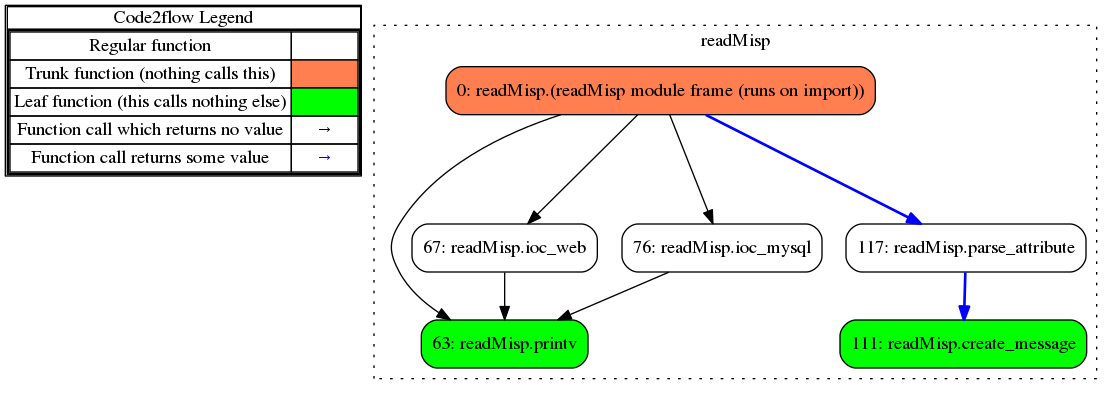
\includegraphics[scale=0.3]{res/flowReadMisp}
	\caption{Code2flow: ReadMisp WorkFlow}
	\label{code2flow-readMisp}
\end{center}
\end{figure}

ReadMisp (fig. \ref{code2flow-readMisp}) will first retrieve the data, either via the web \gls{api}, the MySQL connection or directly from \gls{csv} (located in the res folder). The advantage of the MySQL is the speed for two reasons, first, there is no data transformation as we request the data as it is stored and secondly, in general, the MySQL server is accessible directly from the server that generates the rules which means that there is less network delay.\\
On the flow chart, we can also see the function printv which is a call to print only if the program runs in verbose mode.\\
Once the IOCs are available, the attributes are parsed and the message is created. The message is the important information as it is that that actually identifies the threat and allows the user to connect himself to \gls{misp} and get back all information related to the event.\\
For the parsing is the real creation of the rule, which is done in several steps:

\begin{enumerate}
\item Values from \gls{misp} are split and associated with their type in a dictionary.
\item \gls{url} are normalised.
\item The message is created.
\item The Crypto package is called to create the rules.
\end{enumerate}

In order to be modular, all the code for rule creation is separated. Each time that the program is started, it goes to the configuration file to see which Crypto module to load from the crypto package.\\
All modules need to implement the interface (interface.py) and then must be added in the choose\_crypto.py.\\
For an example, the workflow for the PKKDF module is available in figure \ref{code2flow-pbkdf2} and will be explained afterwards.

\subsubsection{MatchRules}
\begin{figure}[h!]
\begin{center}
	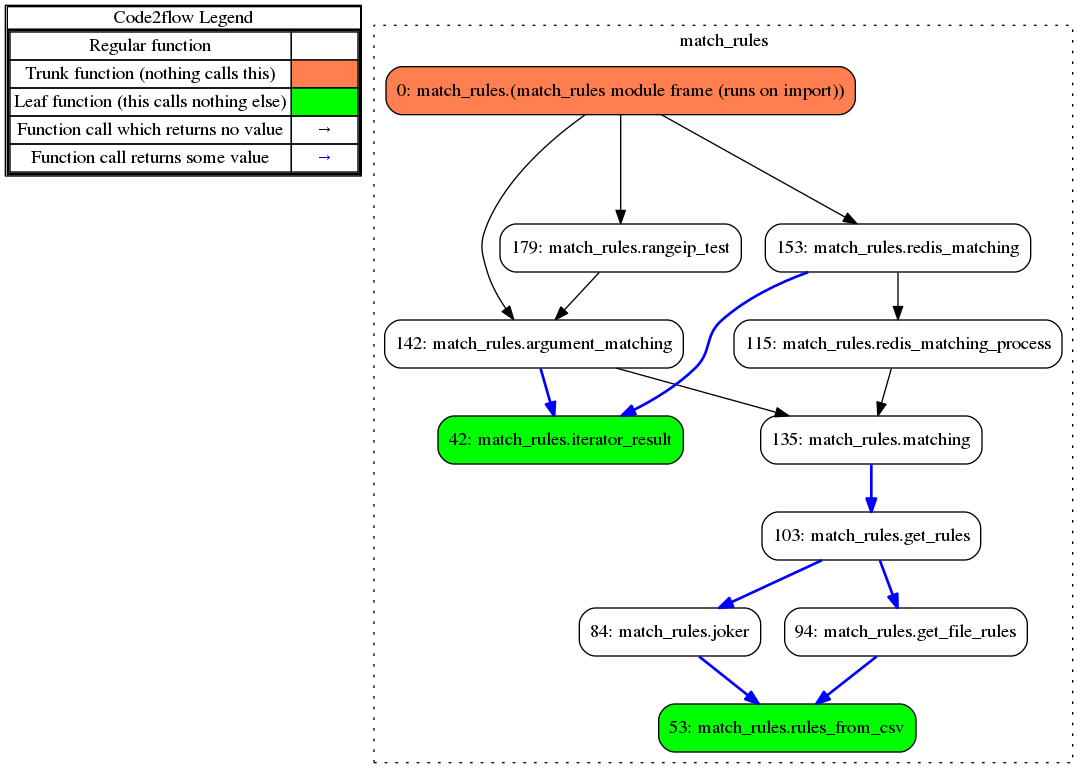
\includegraphics[scale=0.3]{res/flowMatchRules}
	\caption{Code2flow: MatchRules WorkFlow}
	\label{code2flow-matchRules}
\end{center}
\end{figure}

Match rules has two really different ways of working, try to match an element from the arguments (argument matching) or from redis if the system with the logs is used.\\
The additional rangeip test is just for testing purpose and will be further explained in the benchmark sections.\\

For redis matching, the only difference is that a pool of processes running a redis matching process is used.\\
Each process is actually polling the redis queue for new logs and is then feeding them to the matching system.\\
In the other system, the arguments are directly fed to the matching system.\\

The matching system is working in different steps, first, in function of the argument types, it will load and cache the needed rules (get\_rules).\\
There are two types of rules, the standards one are divided into files as well as the 'joker' file for the bloom filter if it exists.

Once the rules are loaded, for each attributes to check, the crypto module will try to decrypt each rule up to find or not a match.

\subsubsection{Crypto Module \gls{pbkdf2}}

\begin{figure}[h!]
\begin{center}
	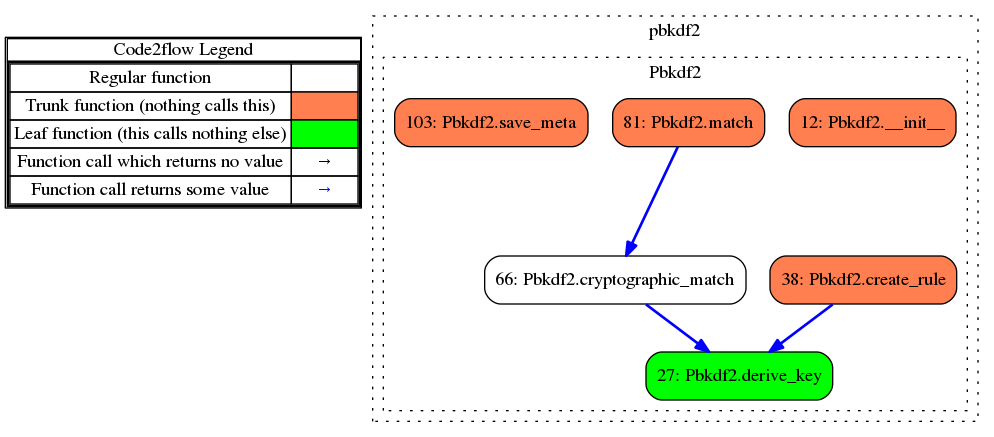
\includegraphics[scale=0.3]{res/flowPBKDF2}
	\caption{Code2flow: PBKDF2 Crypto Module WorkFlow}
	\label{code2flow-pbkdf2}
\end{center}
\end{figure}

\begin{figure}[h!]
\begin{center}
	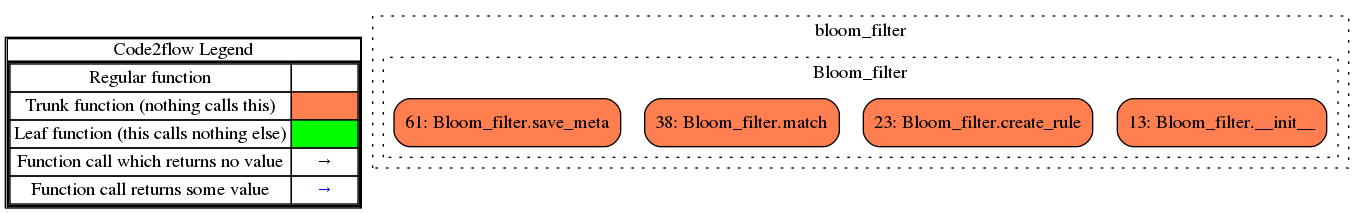
\includegraphics[scale=0.3]{res/flowBloomFilter}
	\caption{Code2flow: Bloom Filter Crypto Module WorkFlow}
	\label{code2flow-bloom}
\end{center}
\end{figure}

The crypto modules are responsible for creating and matching rules. In the particular case of the \gls{pbkdf2} module, it generates the keys and encrypt the message or try to decipher it.\\
I've additionally added the bloom filter chart as well to see that the difference is small as they inherit the same interface.\\

As the types of file can differ from modules to modules, this is also the crypto module wich is responsible for saving data and metadata files.\\
This part can take a lot of time as for saving the elements (as well as getting them) we cannot afford problems inside the files with special characters. So for that the idea is to use base64 encoding for the encrypted message, the salt/nonce and also the cipher-check argument (used for faster match checking).\\


\subsection{Profile of ReadMisp for 1 iteration}
We thus need to verify that generating the keys and encrypting/decrypting data is much more time consuming than everything else even with one iteration.\\
We should also do especially close attention to the normalisation of \gls{url}s. Normalisations could be inefficient as I don't know how the library is implemented and moreover, I'm additionally iterating for searching regex after that which can be inefficient.\\

For profiling the code, I've had some difficulties, first, I tried to use the vprof profiler as it seems to be the best and it was said that it supports python3.\\
But there were a lot of errors and I first didn't succeed in using it. I've thus tried to use a line\_profiler (only working with python2) then profiling which was really complicated to used. \\
I finally managed to use vprof with a little modification (to force it using python3) and I was really impressed by this tool that analyses everything. We can have graphs of the function utilisations, a line by line profile as well as a memory analyse which can be really useful.\\

\begin{figure}[h!]
\begin{center}
	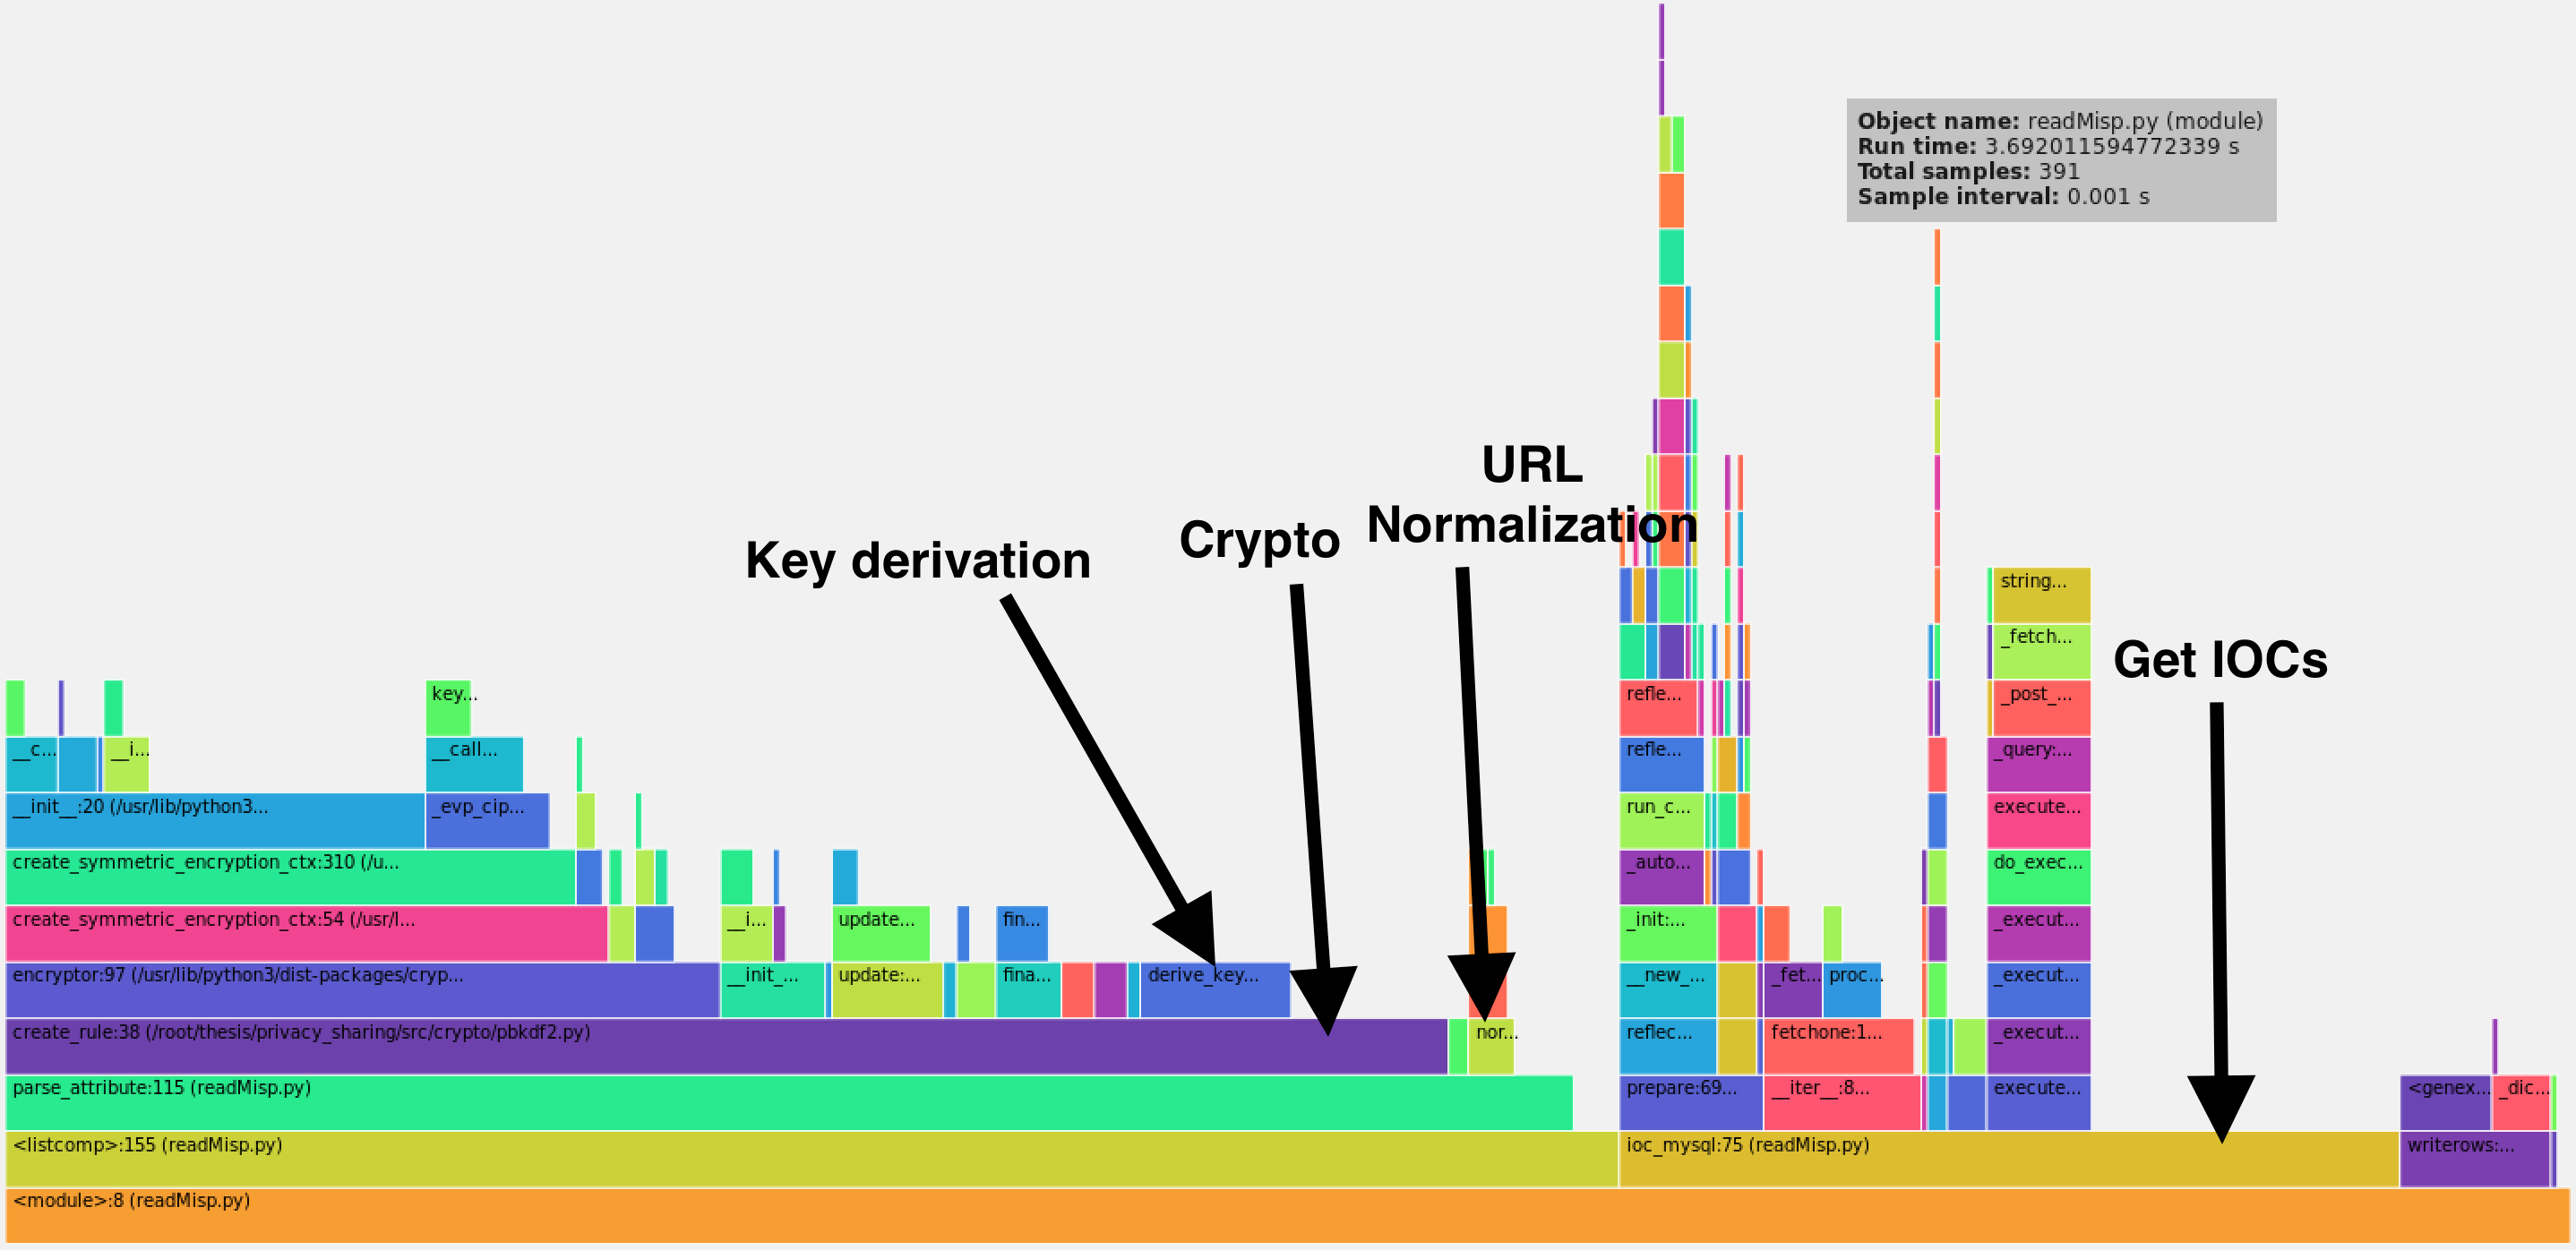
\includegraphics[scale=0.3]{res/profile-1iter}
	\caption{Vprof - Flame Chart Profile of readMisp PBKDF2 - 1 iteration (--misp mysql)}
	\label{profile-readMisp}
\end{center}
\end{figure}

This graph \ref{profile-readMisp} shows that getting the \gls{ioc}s from MySQL takes approximately one-third of the time. And there, we also see that two-thirds of this section are used directly for MySQL but the one-third left is used for ordering and small modifications of the format of some values. This could be slightly improved but this would not increase the average performance as we can see with 1000 iterations.\\
Then writing data to files (Rightmost dark blue) takes time but cannot be improved significantly.\\  
The first question about the normalisation time is answered and we see that it shows that the normalisation process of \gls{url}s is already a small amount of time compared to one iteration for the key derivation.\\
We also see that in this particular case, the major part of the time is taken by the encryption of the messages.

\begin{figure}[h!]
\begin{center}
	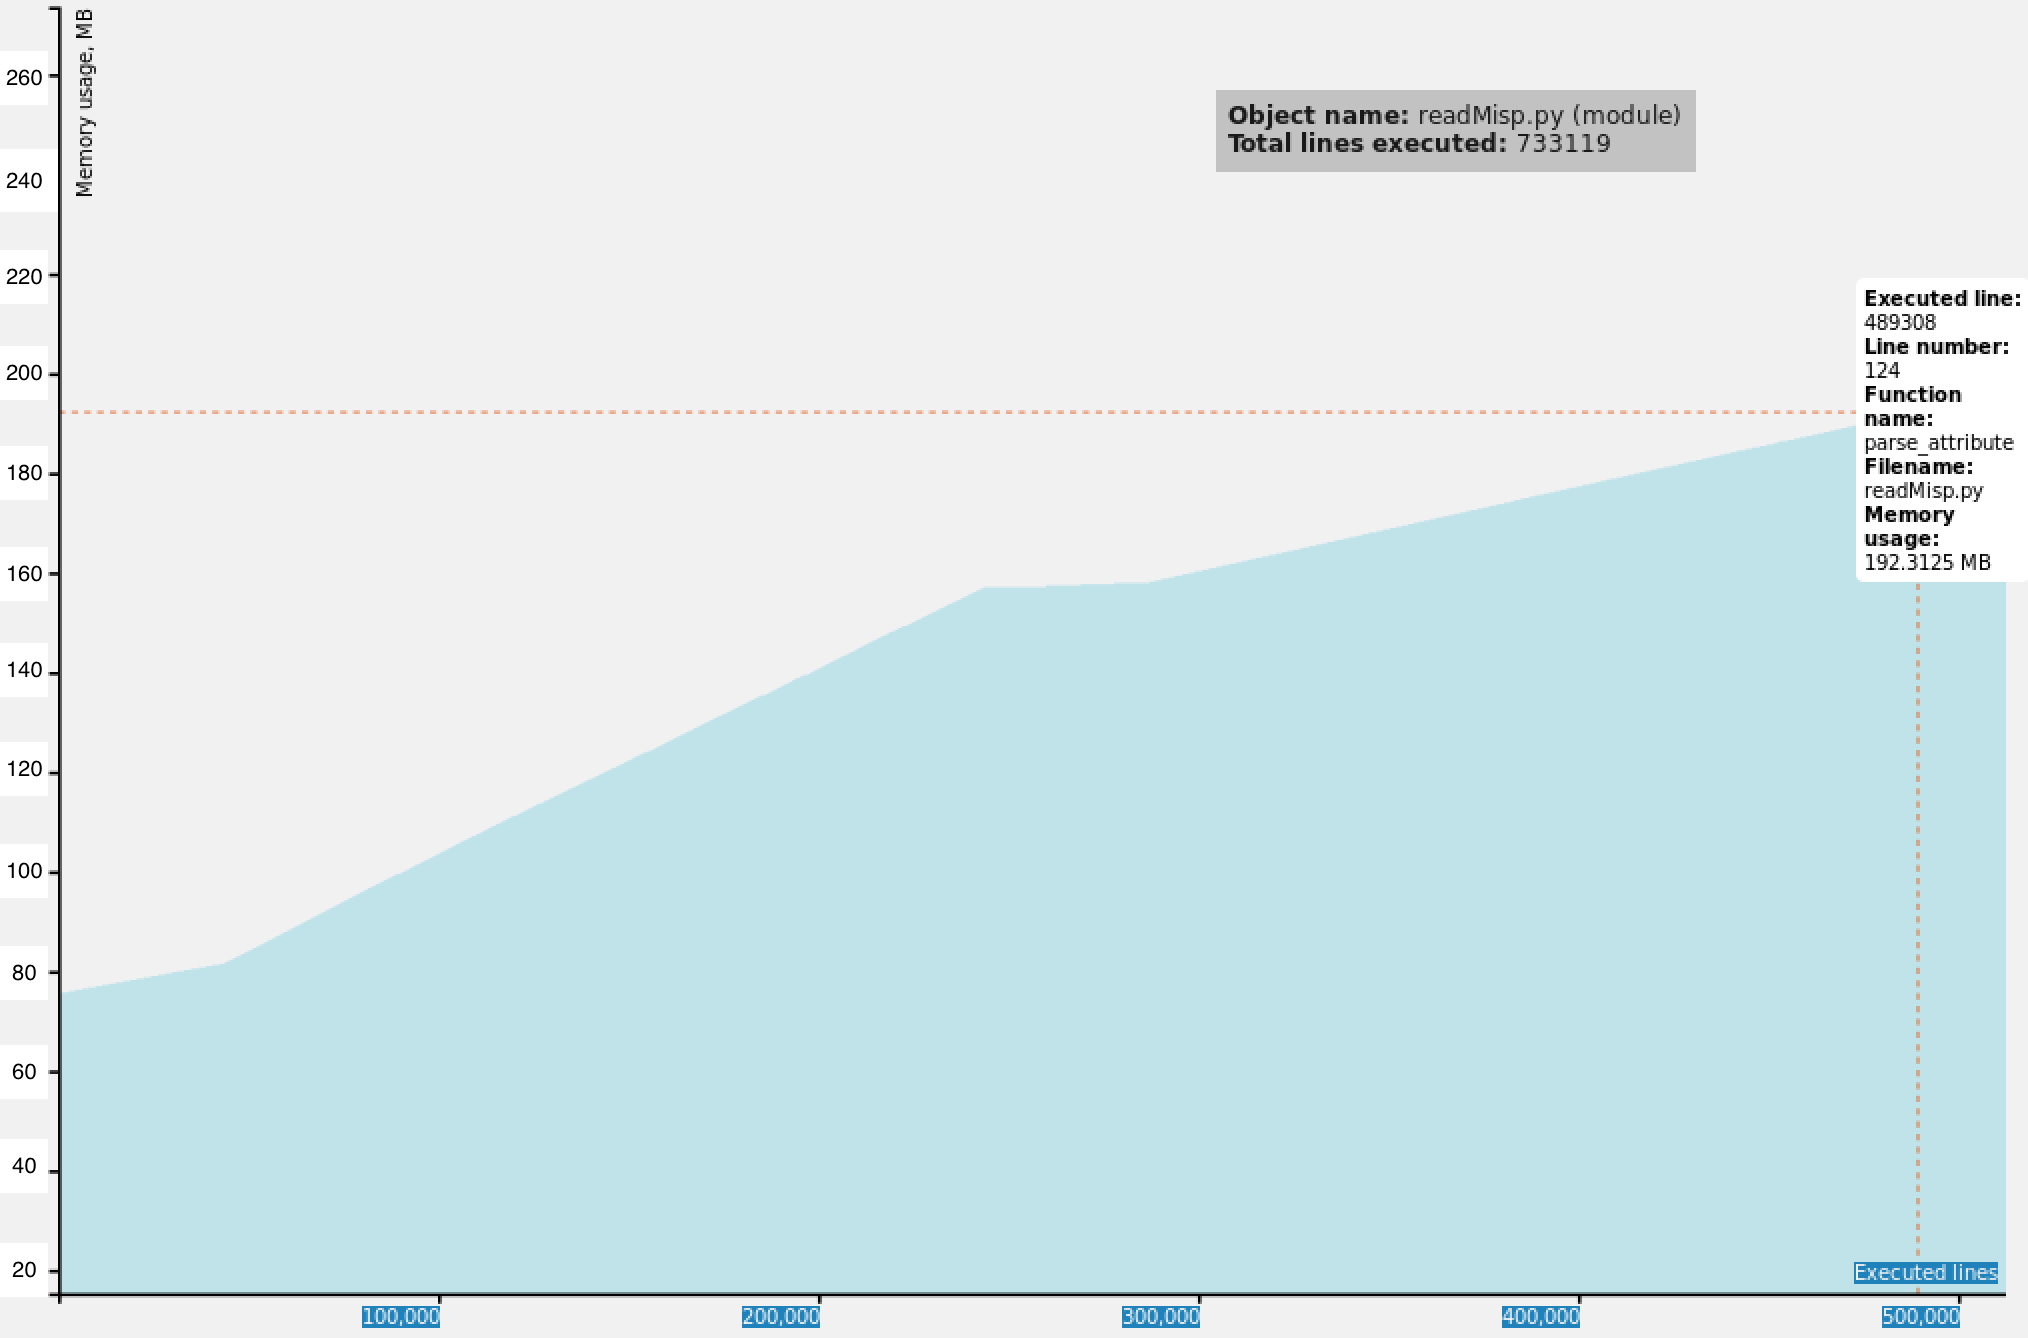
\includegraphics[scale=0.3]{res/profile-mem-readMisp-1iter}
	\caption{Vprof - Memory Chart Profile of readMisp PBKDF2 - 1 iteration (--misp mysql)}
	\label{profile-mem-readMisp}
\end{center}
\end{figure}

The memory graph we can see that the highest level (on the right) is approximately at 200MB used for 27663 rules. This does not vary with the number of iterations.\\ 

\subsection{Profile of ReadMisp for 1000 iteration}

\begin{figure}[h!]
\begin{center}
	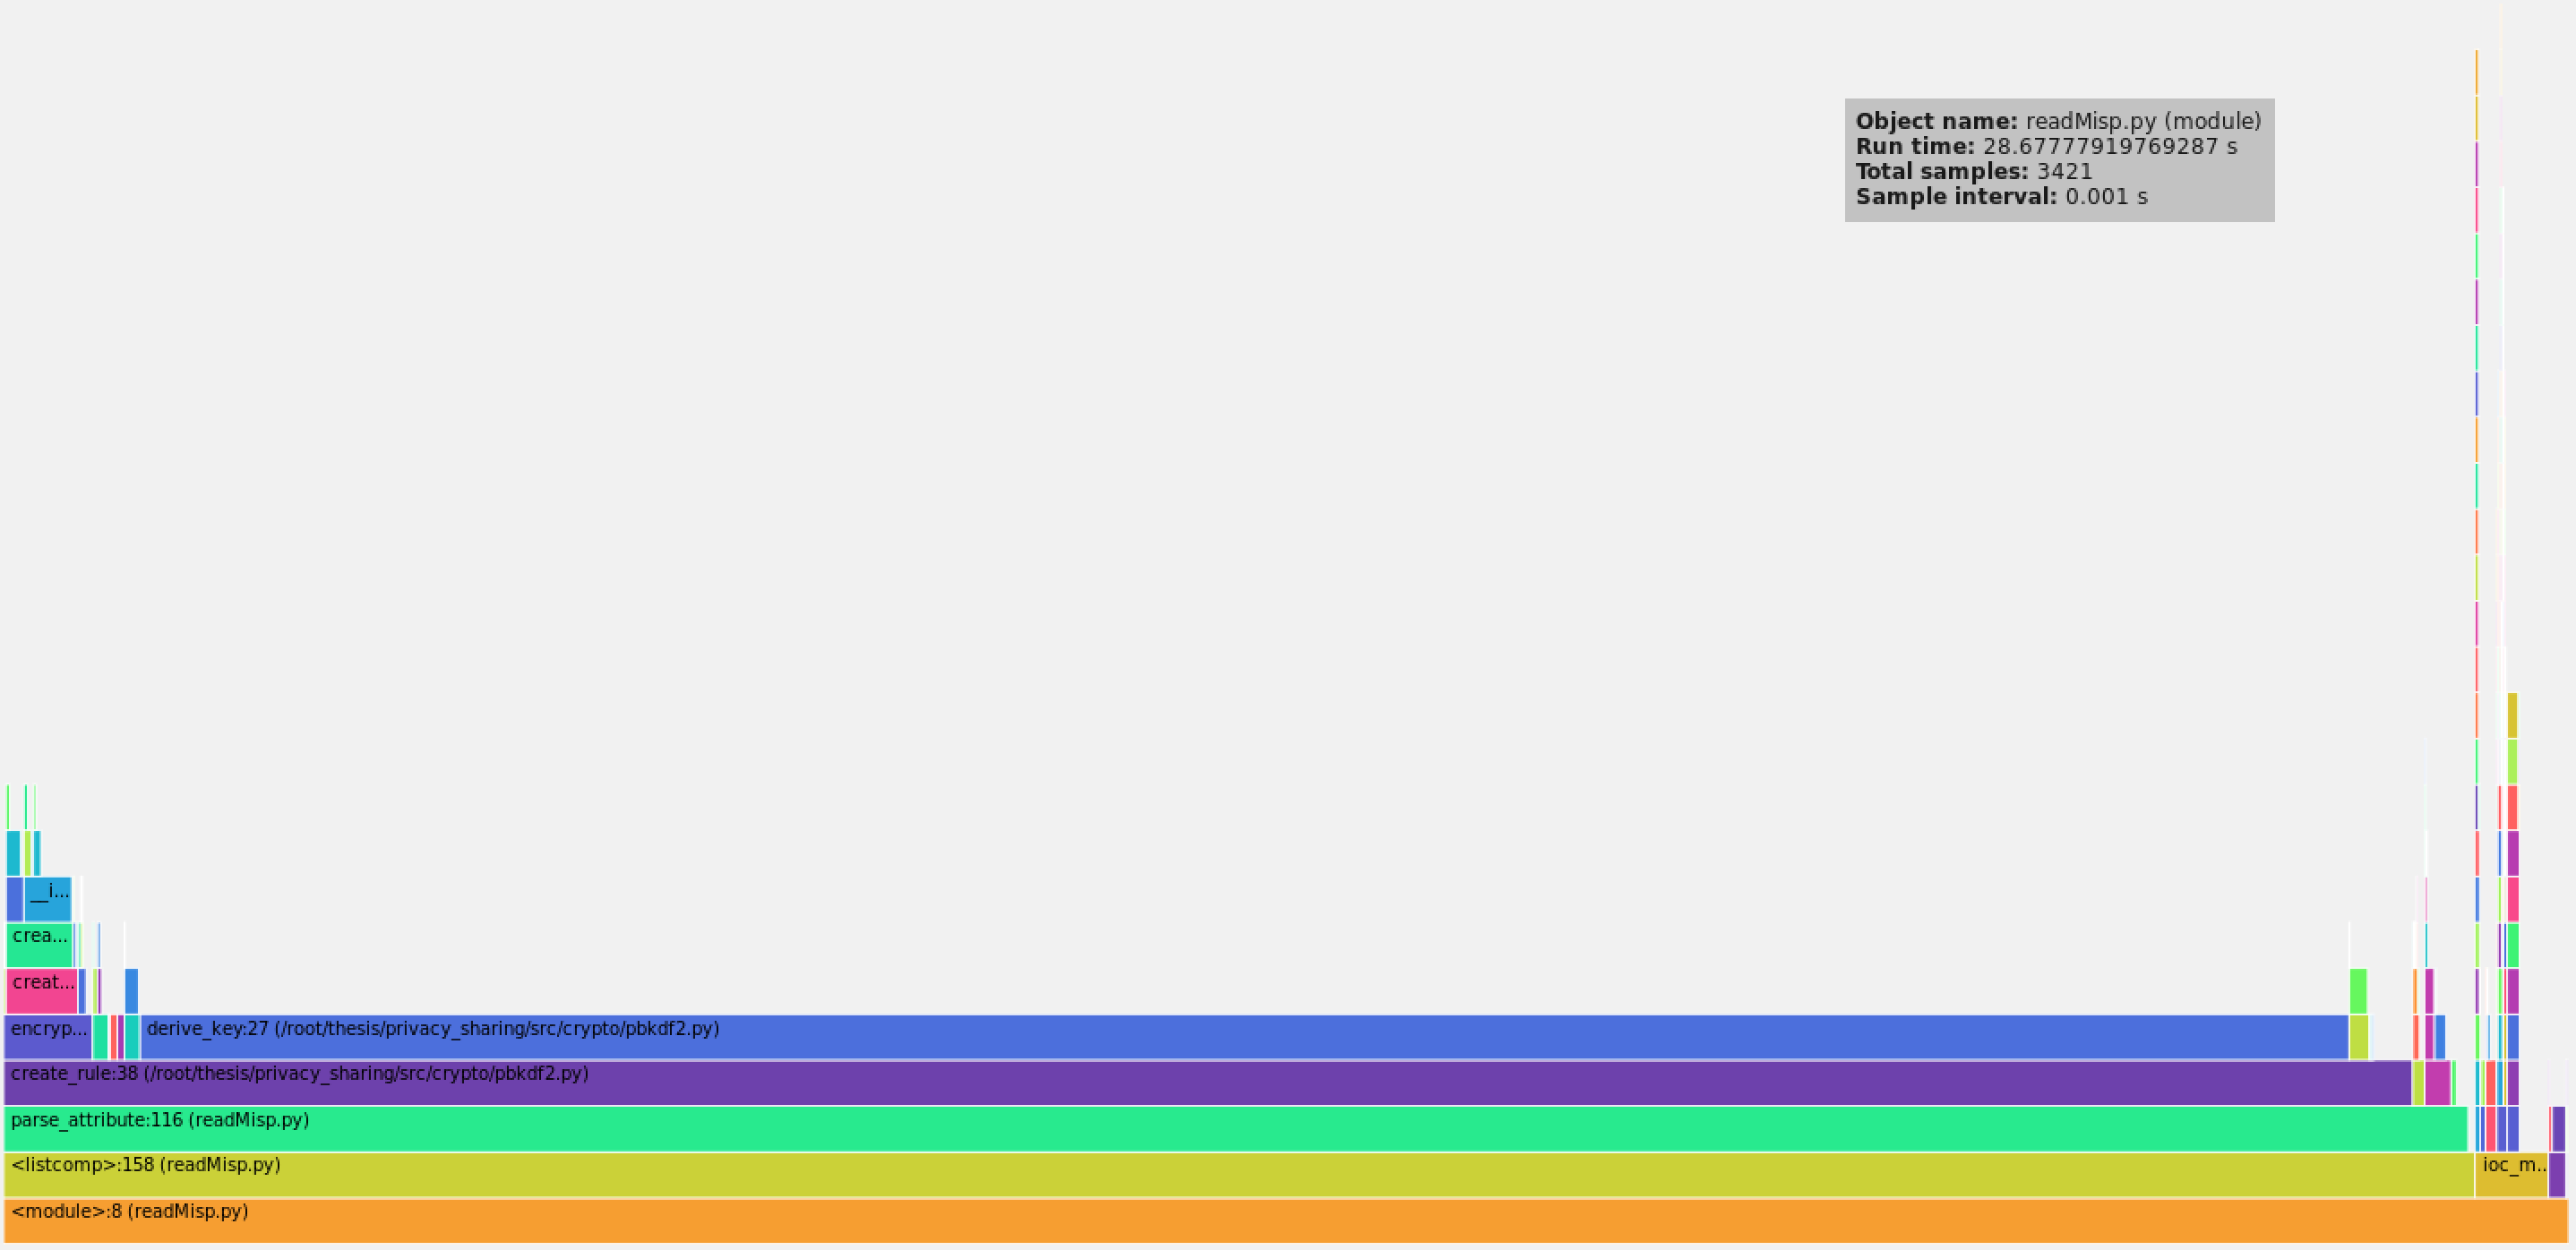
\includegraphics[scale=0.3]{res/profile-1000iter}
	\caption{Vprof - Flame Chart Profile of readMisp PBKDF2 - 1000 iteration (--misp mysql)}
	\label{profile-readMisp1000}
\end{center}
\end{figure}

The goal of this work is to slow down the system, which means that a lot of iterations will be used. This is the reason why this is closer to a real execution of the system. Of course we can see that the major part of the time is used by the key derivation function (fig. \ref{profile-readMisp1000}).\\

\subsection{Profile of the bloomy\_pbkdf2 module}
The first step is to analyse the computationnal overhead for creating the rules with the bloomy module. The figure \ref{profile-bloomy-readMisp-1iter} shows that the key derivation function is still more computationally intensive than the creation of the bloom filter, to be more precise, we can even see that bloom filter generation takes only 1.9\% of the time.\\


\begin{figure}[h!]
\begin{center}
	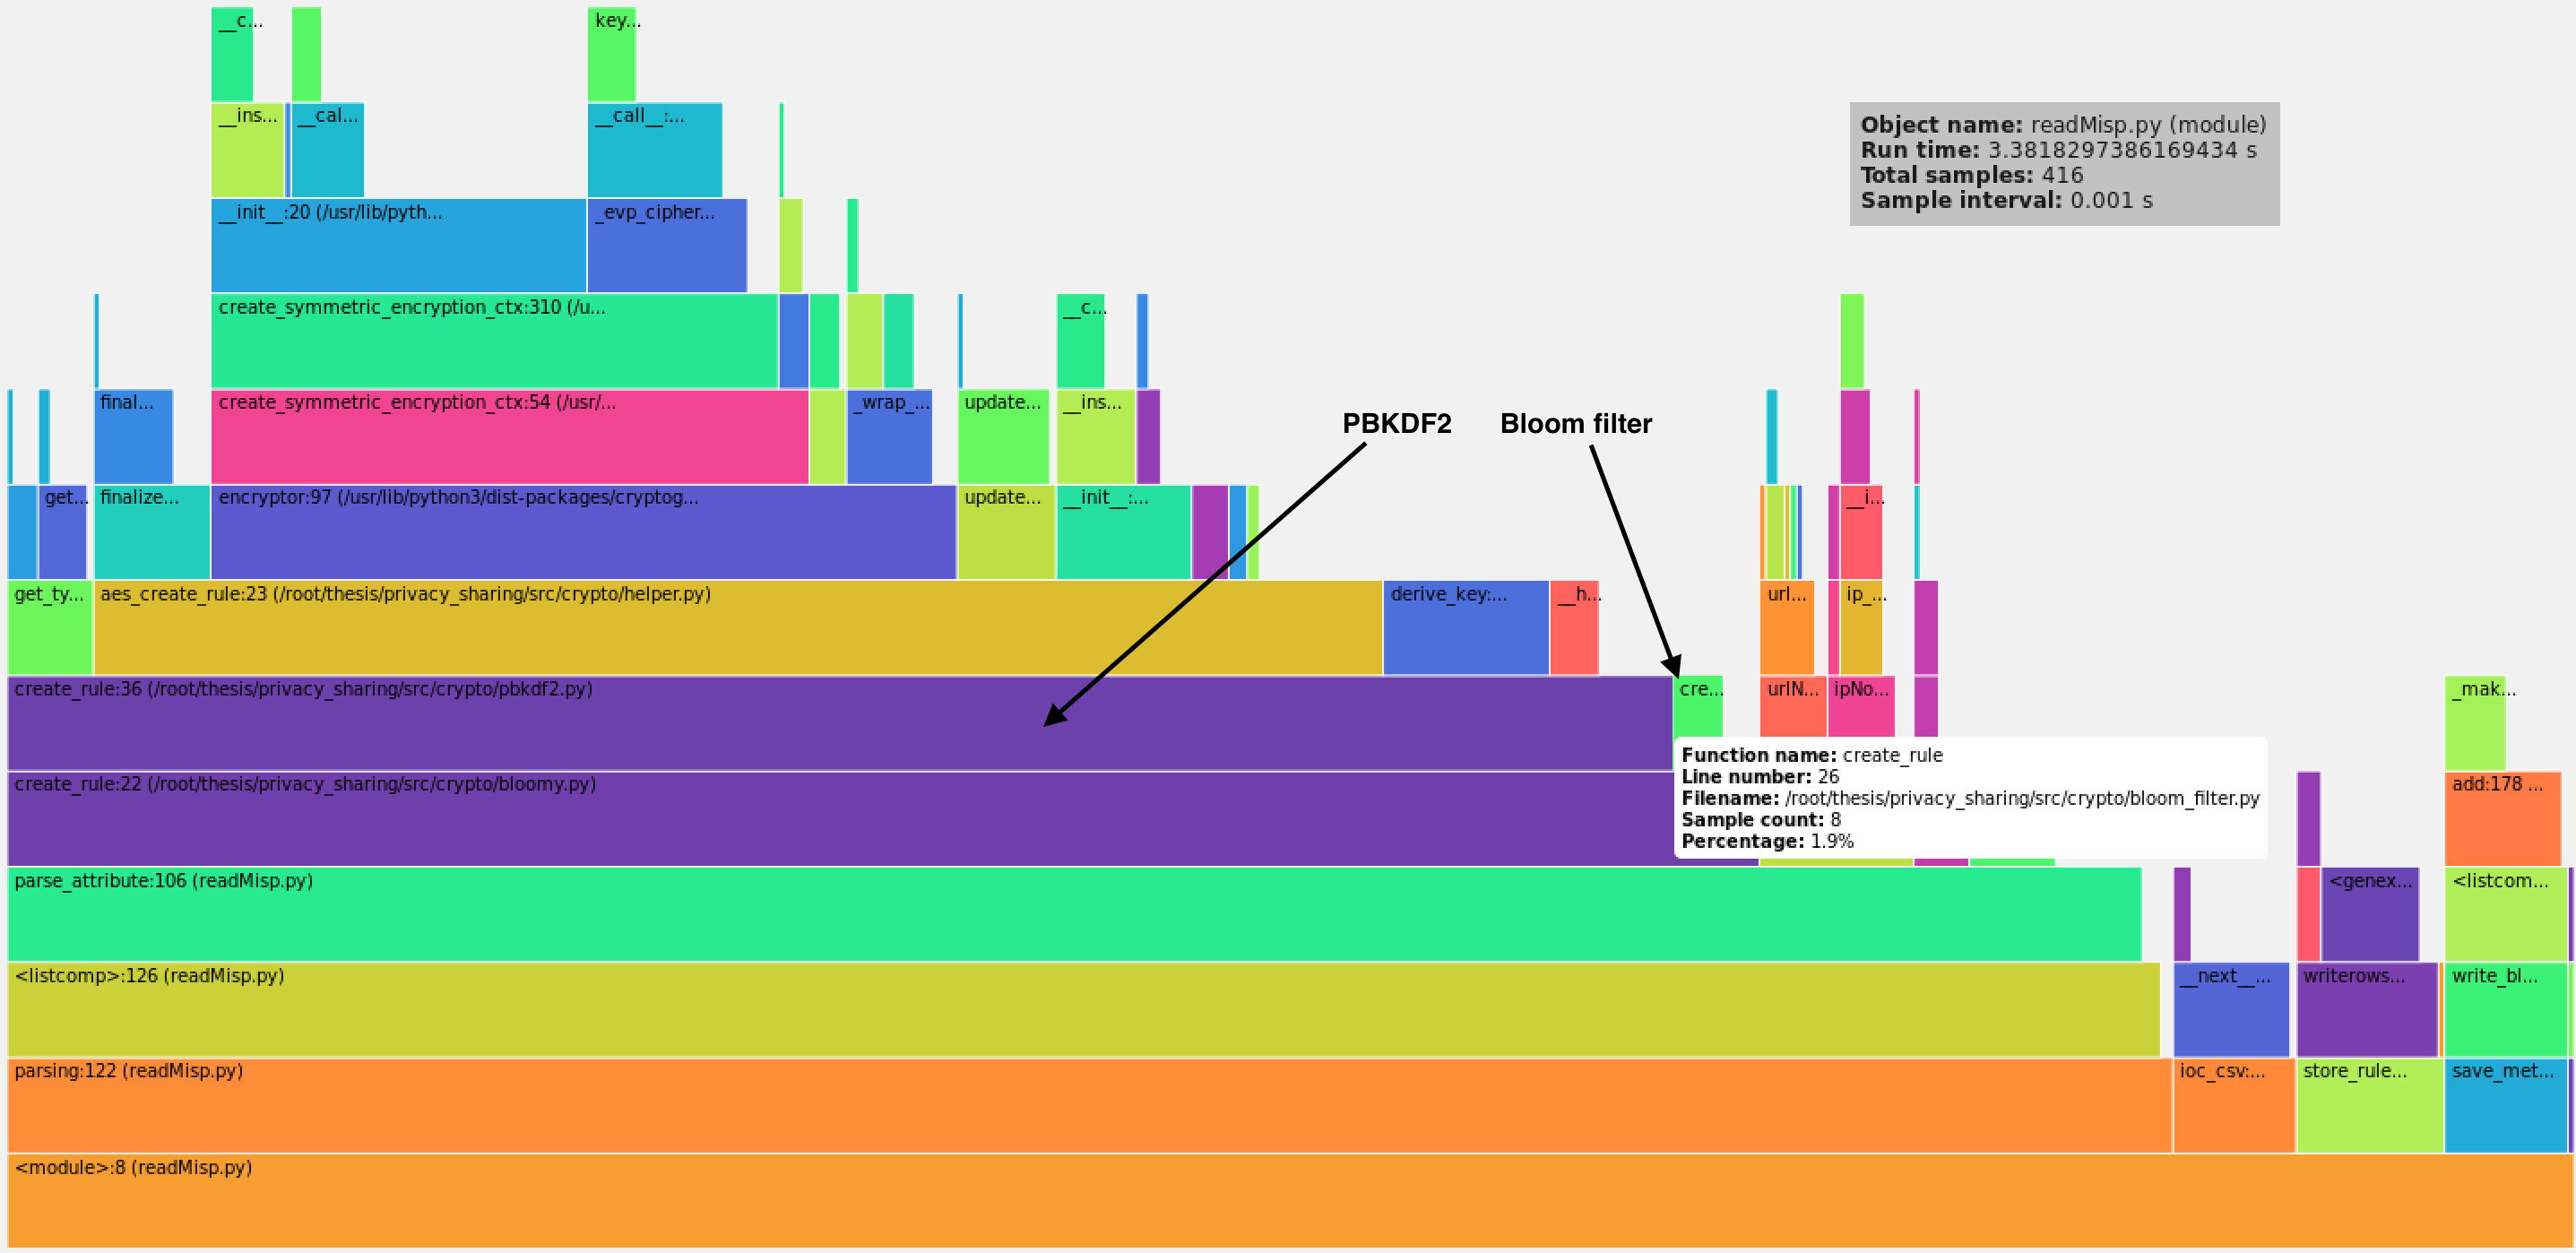
\includegraphics[scale=0.3]{res/readMisp-bloomy-1iter-res}
	\caption{Vprof - Flame Chart Profile of readMisp bloomy\_pbkdf2 -1 iteration (--misp res)}
	\label{profile-bloomy-readMisp-1iter}
\end{center}
\end{figure}


Then, when the code is running, there are three existing paths for checking a value. Firstly, if there is a match, due to the 0 rate of false negative, we know that the bloom filter will match. Then All rules will be checked and the match(es) will be found. On the other side, if there is a match, there are still two possibilities. Either the bloom filter matches due to its false positive rate and therefore all rules will be checked as well or, the bloom filter will reject the membership and it is the special case that improves the overall performance of the matching system.\\


\begin{figure}[h!]
\begin{center}
	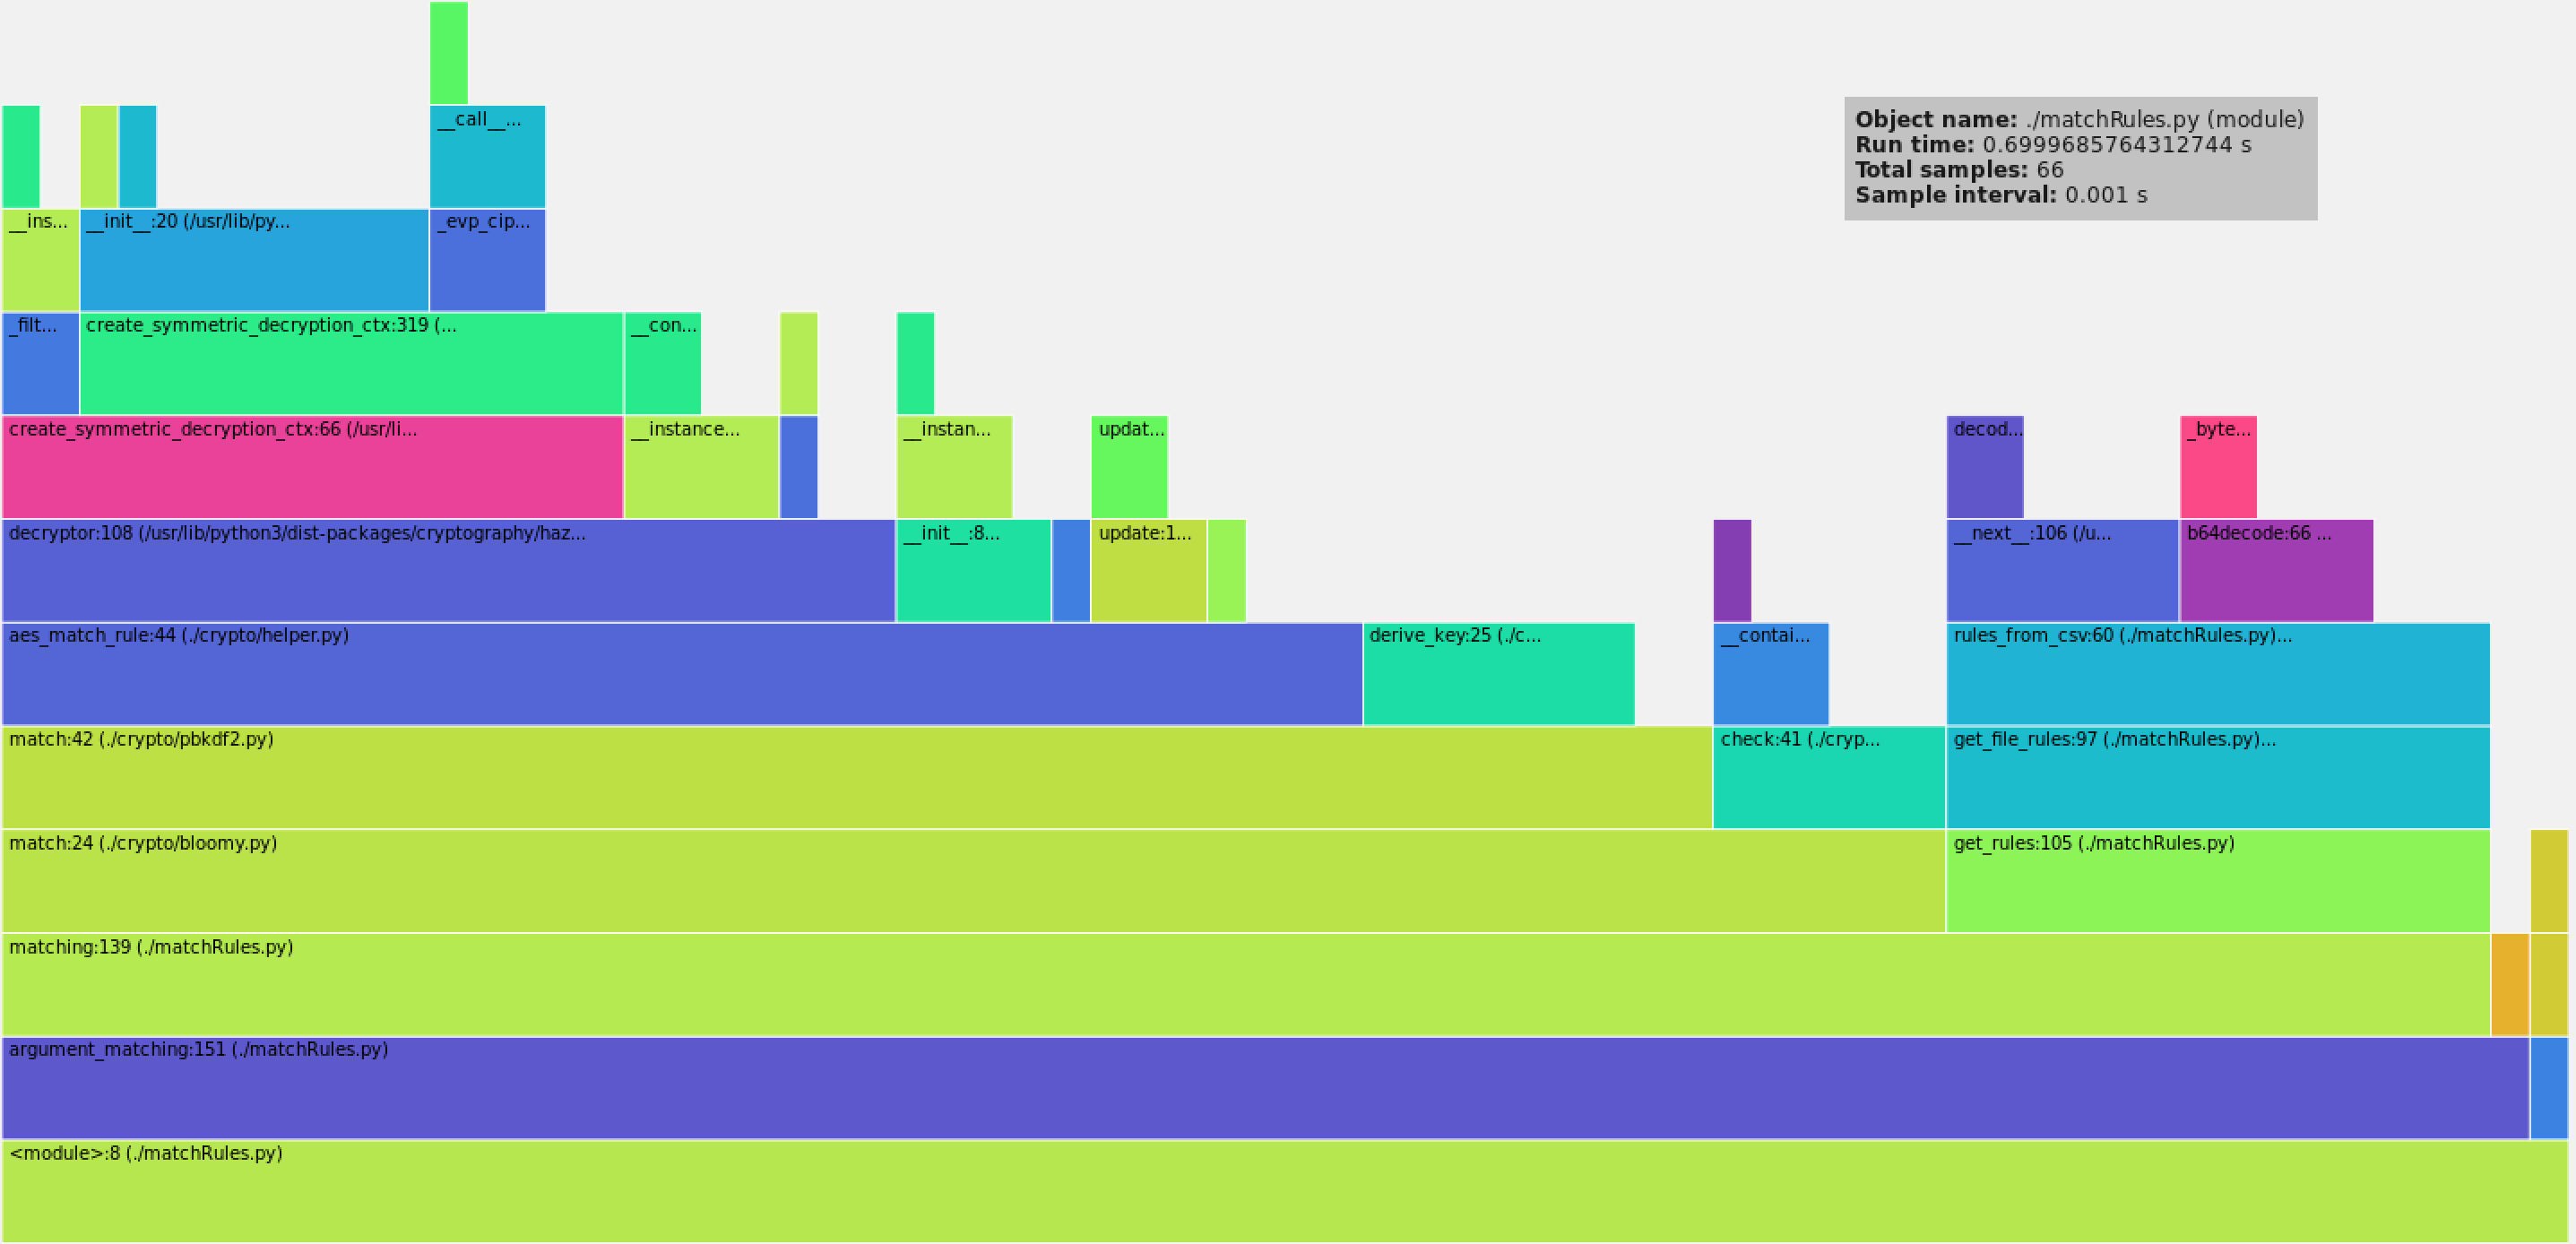
\includegraphics[scale=0.3]{res/match-exist}
	\caption{Vprof - Flame Chart Profile of matchRules bloomy\_pbkdf2 (1 iteration) with a match}
	\label{profile-bloomy-match}
\end{center}
\end{figure}

On figure \ref{profile-bloomy-match} we can see that it takes more time than the simple \gls{pbkdf2} module as we have the overhead of the bloom filter. This is exactly the same behaviour when there is no match but a false positive bloom filter match.\\

\begin{figure}[h!]
\begin{center}
	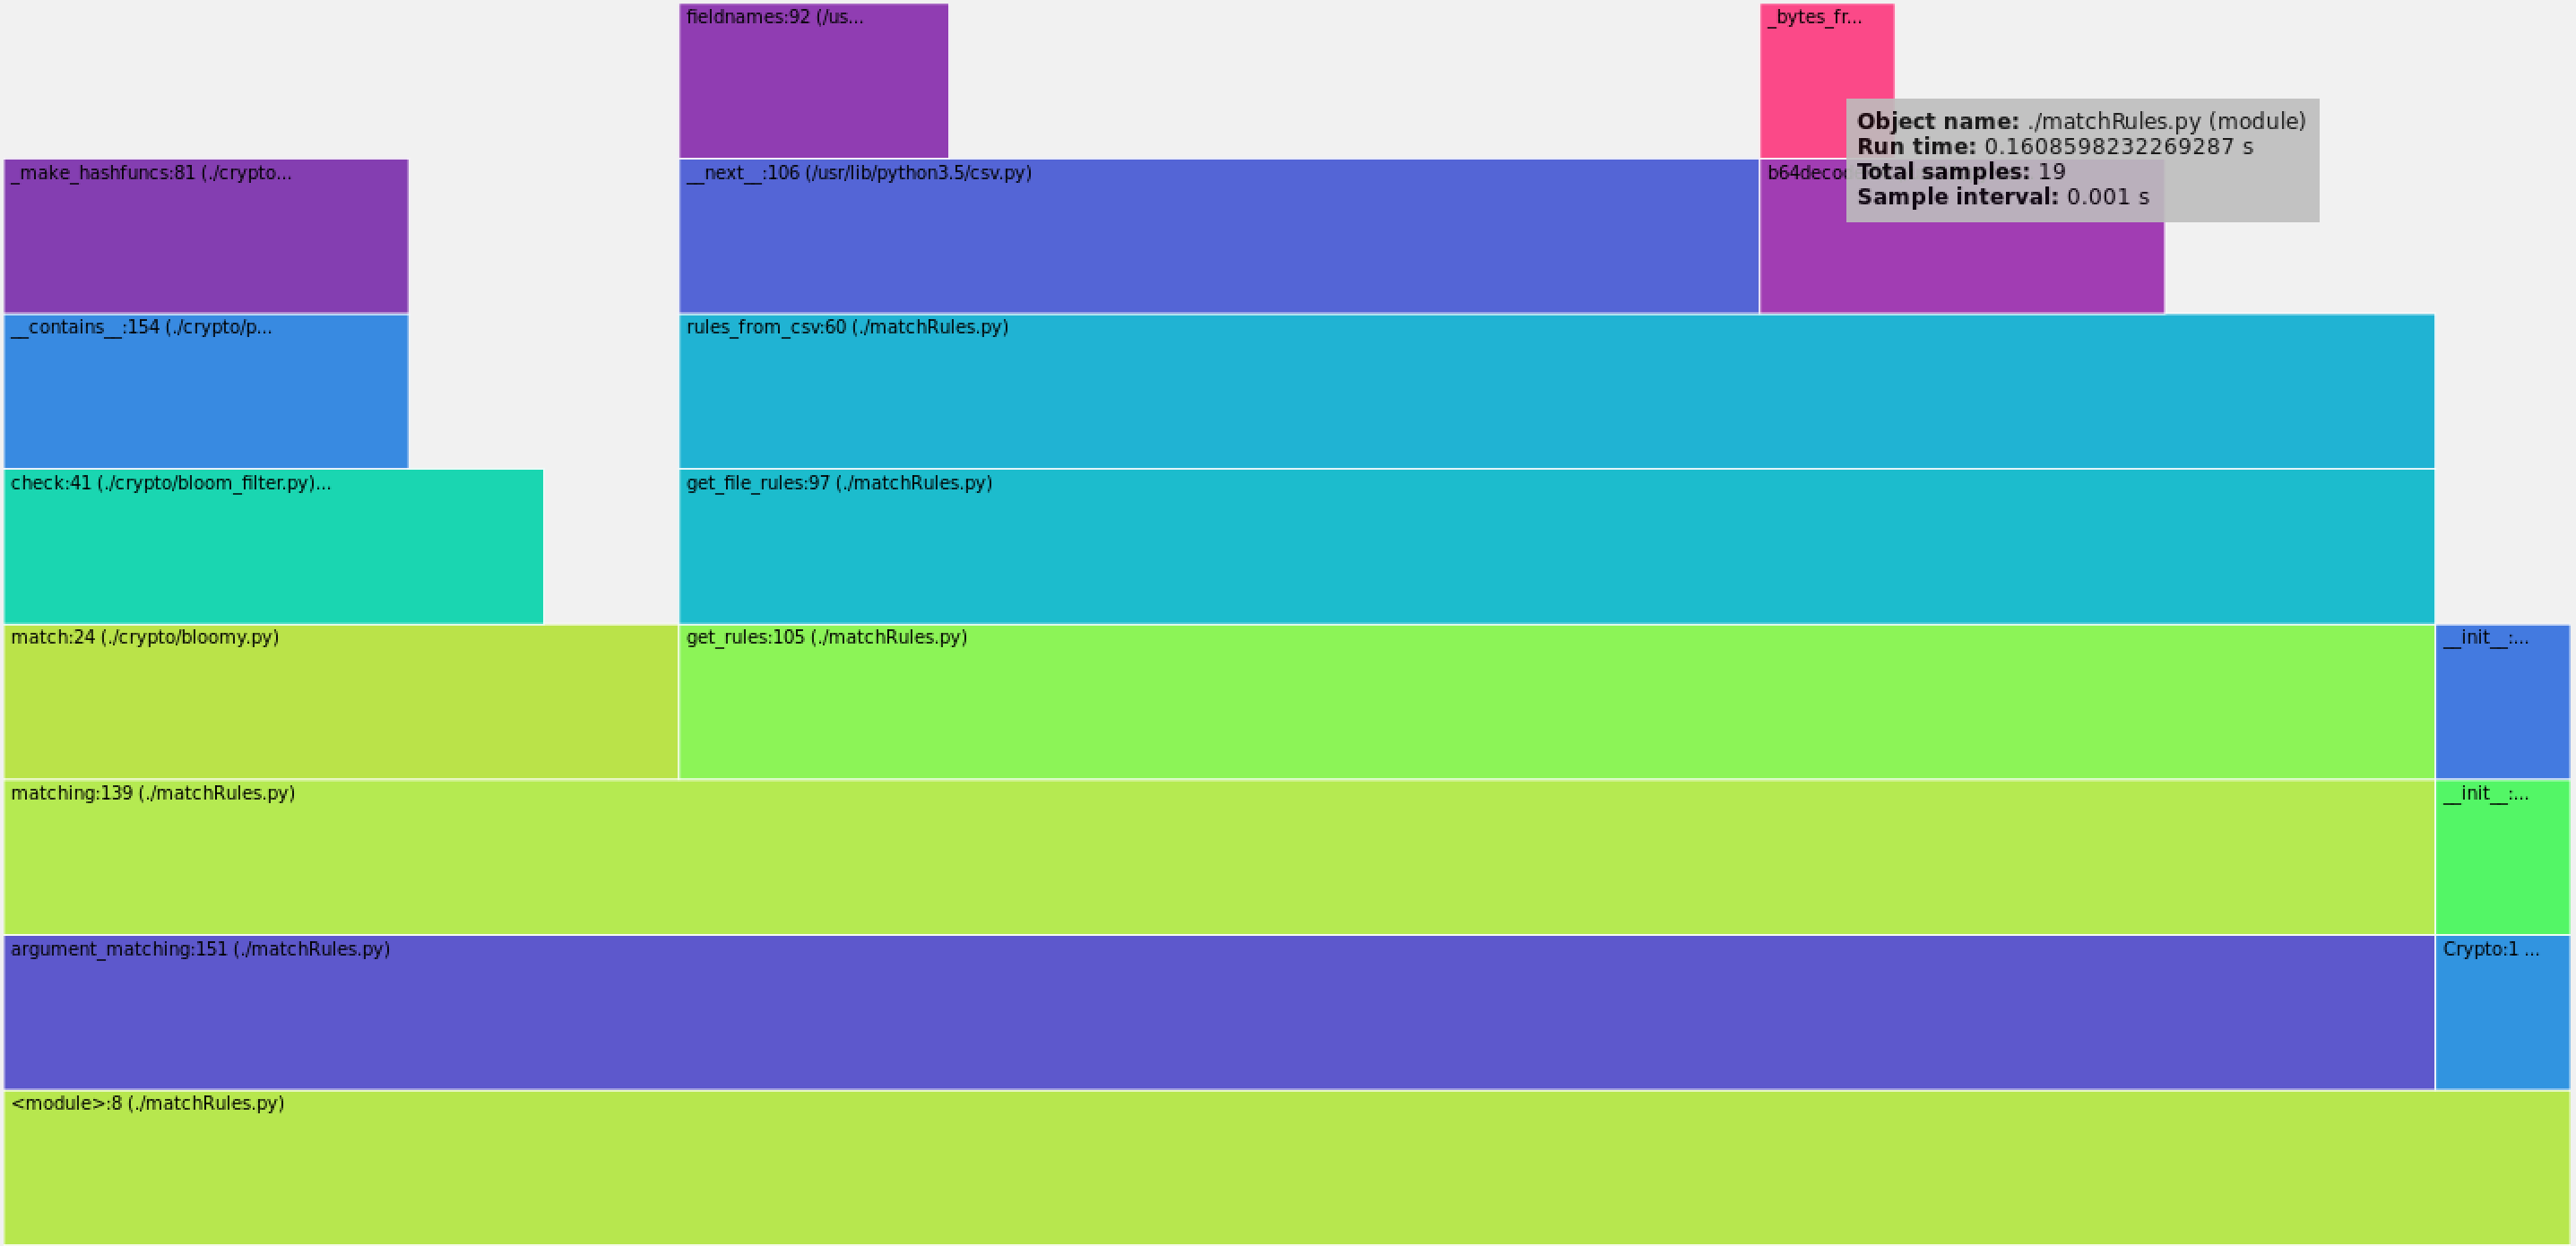
\includegraphics[scale=0.3]{res/match-bloom-not}
	\caption{Vprof - Flame Chart Profile of matchRules bloomy\_pbkdf2 (1 iteration) with no match in the bloom filter}
	\label{profile-bloomy-no-match}
\end{center}
\end{figure}

While we can clearly see the advantage of the system in the figure \ref{profile-bloomy-no-match} as the bloom filter immediately realise this value does not belong to the set.\\

In this case, we can realise that there is a problem with the implementation, as I tried to have a modular implementation and doing everything inside the modules, it does not always goes well with the system. Here, for one attribute, whatever the result of the bloom filter for one rule it will test the bloom filter for every different rules. This is really bad as the bloom filter is not related to the rule but only to the attribute tested. To solve this problem a cache must be implemented. The first cache implementation already improved the system but was really bad as I was using a dictionary of matched values.\\
There are two problems with that, first, to put the orderedDictionary used for representing an attribute as a key, we need to transform that into a string. And then add it to the cache.\\
But for a matching, we each time need to transform the value to a string and while checking the dictionary it actually hashing the string attribute. All that was taking a way too much time and I finally opted for a simple but nevertheless efficient implementation with only two cache variables, the last OrderedDictionary representing the attribute to check with the last bloom filter result.\\
This cache is so fast that the bloomy overhead does not appear any more on the profiles, the script complete run when bloom filter discover the attribute is not in the set is about 0.16s.\\

\section{Benchmarking}
The ideas have been explained, in the first few sections, then the implementation had been explained followed by profiles that help to understand the behaviour of the system and how the computation power is used inside the system. Now it is time to see how it is working with real data, what would be the right parameters to use and why these choices. Moreover, this is in this section that we could analyse if the goal had been totally reached, reached for some part and decide if it can or cannot be used in real implementations.\\
This is important as we are aware of the benefits that it could have but we must stay aware of the risk of that exposure on which a system like this one could lead.\\

\subsection{General Security Discussion}
The standard implementation had already been assessed in the paper  but there is something quite new which is the use of the bloom filters inside the implementation.\\
The goal here is to hide that we have the information, but it is even more to hide who have seen this particular \gls{ioc} and what did they concluded on it.\\
If someone want to test if a specific value is known by the system. First, he needs to get the generated rules. Secondly, to be sure he is the only one to use these rules, its secret token is include in the rules creation what makes them unusable for someone that does not knows it. it also allows to trace back the origin of a data leak.\\
Once they have these rules and the right token. They can ckeck the value. So if an attacker manage to get those, he can succeed in knowing if specific values are known and to get information allowing him to fetch the information on the \gls{misp} web interface. Which means that, at that moment, there is again a barrier as he needs to have the right credentials to get more informations.\\

Therefore we know that we could possibly (but already difficulty) imagine that this system can leaks two important information to an attacker. The number of elements known by the system as well as the fact that someone belonging to an organisation linked to the instance or to some data feed used by the instance have knowledge of a value that the attacker has chosen.\\
This brings a problem with \gls{ipv4} as the number of possible \gls{ipv4} is limited but it seems unfeasible to bruteforce longer data like \gls{url}s.\\

On the other side, if someone wants to attack himself directly to get information from one rule. It is nearly impossible. If the attacker want to bruteforce the ciphertext, he first needs to be able to break an \gls{aes} encryption scheme with a 128-bit key. And then it could get the message but still not the \gls{ioc} related to the information.\\
To get the \gls{ioc}, he would still need to be able to reverse the hash function used.\\

With a bloom filter we can therefore increase the matching efficiency for a standard user while giving up an advantage to the attacker. But an advantage that gives him only information that he would have finally found.\\

So in this case, what is important is to benchmark the time used to generate a rule in function of the number of iterations or of the algorithm used. The space memory needed for the rule. The time used for testing an element against a rule.\\
And this, with or without bloom filters. Then it is also important to assess the advantage of the bloomy implementation in function of the number of available rules, the number of iterations and especially the false positive rate used.

\subsection{Key Derivation Functions}
\label{sec:KeyDerivationFunction}
In rules generation and matching algorithm, the \gls{kdf} is the most costly function. For this reason, I've decided to analyse their behaviour in function of the length of the initial value as well as the time complexity used (iterations or rounds).\\

I was first very surprised, as I could see that the length of the key has no impact on the time used to generate the values and that for the two algorithms. Thus, in this section, I will only present the graphs about the impact of the number of iterations and rounds.\\

Also, for both implementations, there are glitters. Even each point is the result of a mean on 100 points, they are probably due to system interrupts.\\

\subsubsection{\gls{pbkdf2}}
As we can see on figure \ref{benchmarking:timePBKDF2} the time increases linearly in function of the number of iterations.
\begin{figure}[h!]
\begin{center}
	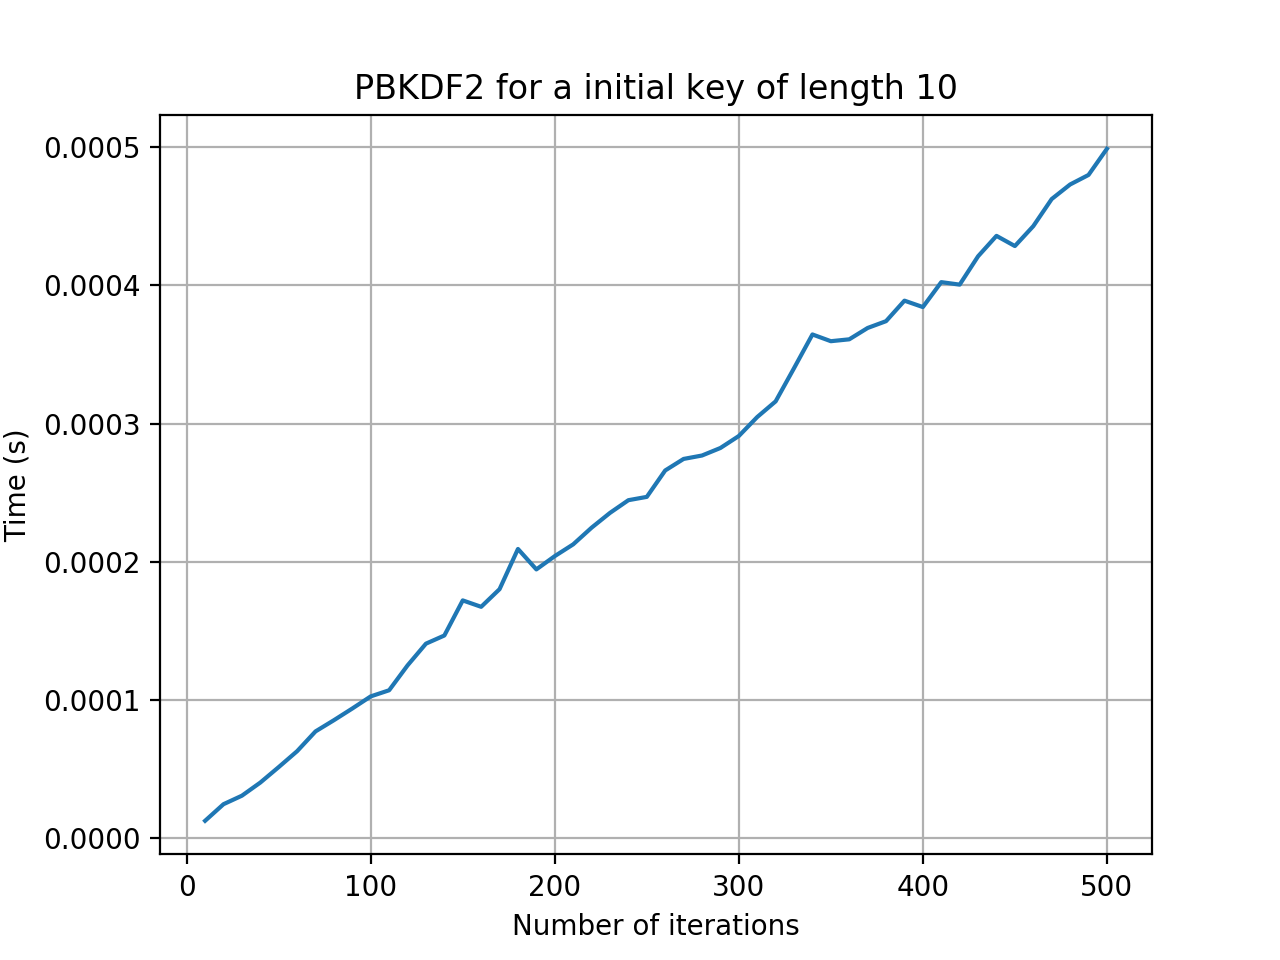
\includegraphics[scale=0.6]{res/TimePBKDF2}
	\caption{Benchmarking: Impact of the number of iterations on the key derivation algorithm PBKDF2}
	\label{benchmarking:timePBKDF2}
\end{center}
\end{figure}
As it is linear, it means that each iterations takes the same amount of time to be computed and therefore, we can approximate that the time needed for generating a password with one iteration is about $10^{-6}$s.

\subsubsection{Bcrypt}
As we can see on figure \ref{benchmarking:TimeBcrypt} the time also increases linearly in function of the number of rounds.
\begin{figure}[h!]
\begin{center}
	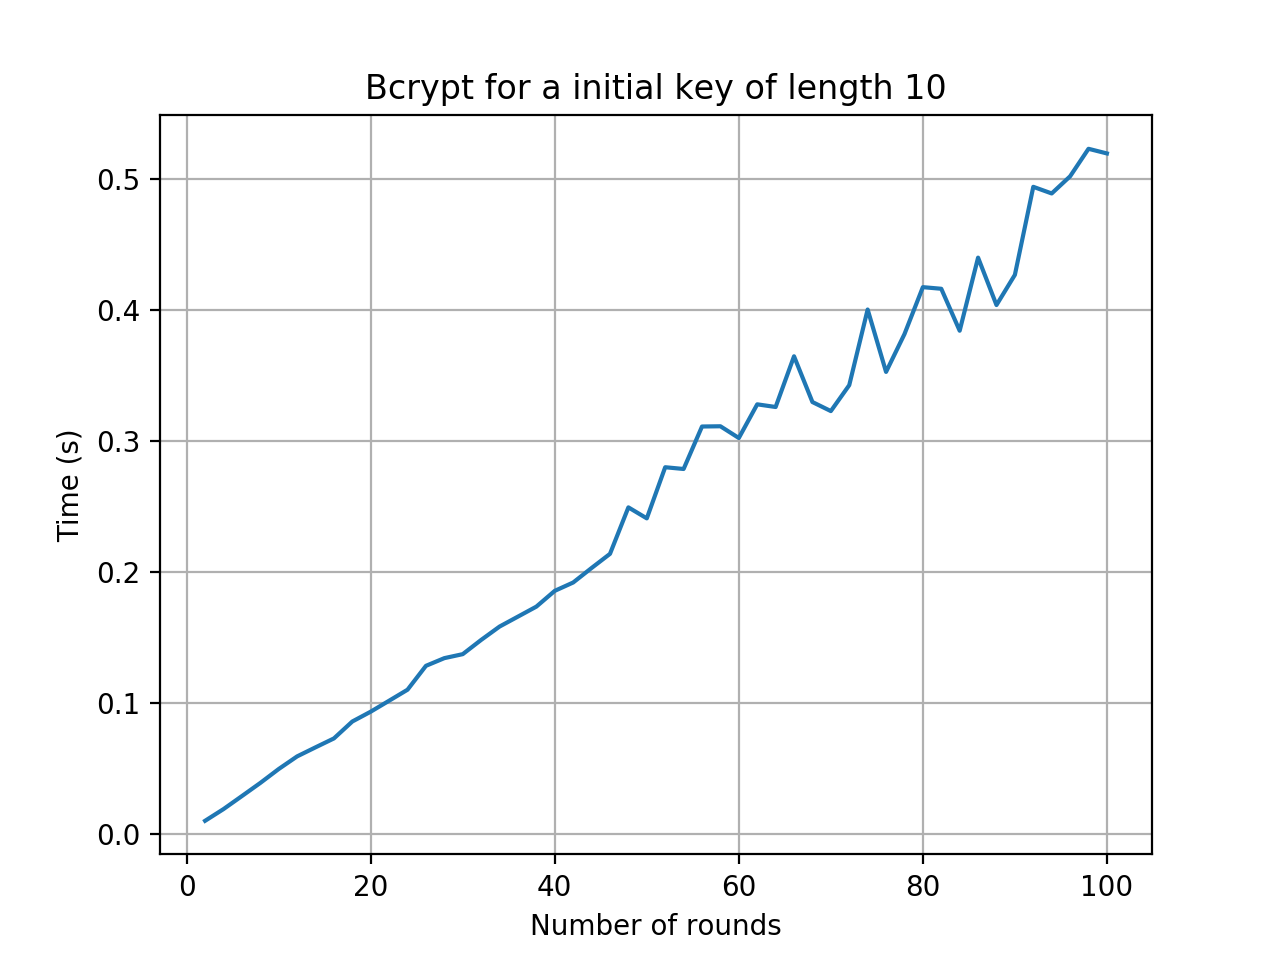
\includegraphics[scale=0.6]{res/TimeBcrypt}
	\caption{Benchmarking: Impact of the number of rounds on the key derivation algorithm Bcrypt}
	\label{benchmarking:TimeBcrypt}
\end{center}
\end{figure}
The same kind of approximation can be done and we get a 0.005s by iteration.
\subsubsection*{Conclusion on \gls{kdf}}
Both algorithm used behaves similarly, the key derivation cost do not varies with the length as well as it varies linearly with the cost parameter.\\
The only observed difference in these graphs are that for the same cost parameter, Bcrypt takes much more time which is better to slow down a bruteforce attack.\\
As the behaviour is similar, the conclusion would be similar as well for both \gls{kdf}. Therefore the following benchmarks will be done only with \gls{pbkdf2}.

\subsection{Bloomy efficiency}
\label{sec:BloomyEfficiency}

Bloom filters are really efficient and used in this context, they allow to make the matching system a way faster. To characterise this improvement, I need to find comparable data.\\
Comparable mean data that are similar in the type of content and on the size as well as easily generalisable. It could have been strings of a fixed size n with a smaller alphabet like \{a,b,c\}. But I have chosen \gls{ipv4} to use this benchmark as well to analyse the feasibility of  bruteforcing them.\\
After that, I needed to decide a number of \gls{ip}s to go through at each step. It needs to be not to small to have precise results but not too much as well to avoid waiting to long for the results. Therefore I have decided to take ten "/24" ranges which means 2560 \gls{ip}s. I have chosen to use 192.168.0.0/24 up to 192.168.9.0/24.\\
Thus for each configuration, the matchRules script ran though all these \gls{ip}s like a bruteforcing algorithm would have done it.\\

The written benchmark was originally created and launched on a virtual private server hosted in France where I ran during a few days before I realise there were an error in the code and that I needed to start over. Then after that I ran into trouble with the instance and reinstalling didn't worked correctly.\\
The final benchmark were than ran on an old computer with 4GB of RAM and an intel i7 processor.\\
I've tested with it the \gls{pbkdf2} module and its bloomy mode for different \gls{fp} Rate with an increasing number of ip-dst (destination \gls{ip}) rules and and increasing number of iterations.\\

As we need to try to decrypt the the whole set of rules in the \gls{pbkdf2} module, it is normal that the time increases linearly with the number of \gls{ip}s in the system. But it is interesting to understand and see the behaviour of the time in function of the number of \gls{ip}s in the system for the bloomy implementation (fig. \ref{benchmarking:timeips}):

\begin{figure}[h!]
\begin{center}
	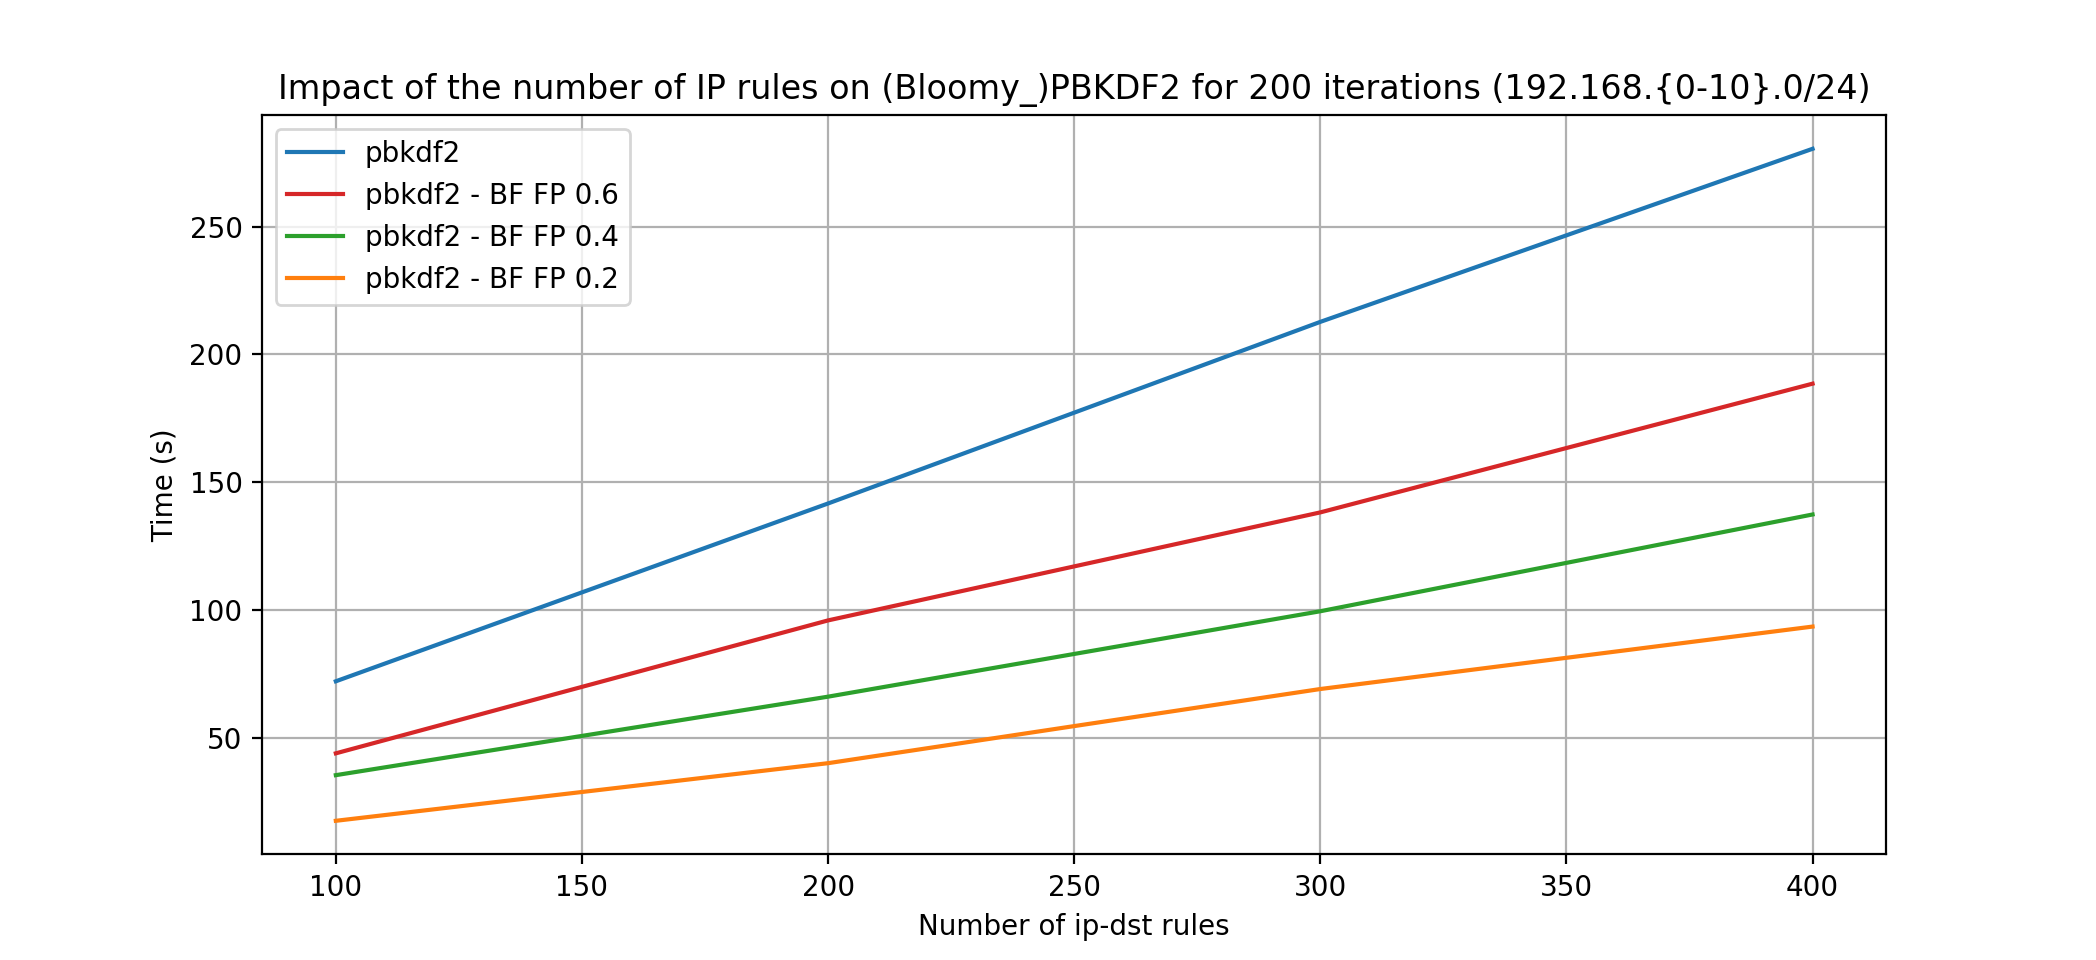
\includegraphics[scale=0.6]{res/TimeIPs}
	\caption{Benchmarking of the evolution of the number of IPs in the system}
	\label{benchmarking:timeips}
\end{center}
\end{figure}

The figure shows clearly a linear behaviour for the four \gls{fp} rates (\gls{pbkdf2} without bloom filter can be considered as a False Positive rate of 1). The only difference is the slope. We can notice that less is the False Positive rate less is the slope is.\\
We can see as well as for example the version without bloom filter is approximately twice longer than the version including a bloom filter with a 0.4 false positive rate.\\

This resulted benchmark seems corresponding to what should be expected as, knowing that for the simple \gls{pbkdf2} it took 847.42s for 200 ip-dst rules (nIP), 700 iterations (nIt) and that we test 2560 IPs (nIPTested):
\begin{itemize}
\item[•] Time needed for testing a an \gls{ip} on a rule is $\frac{Time}{nIPtested * nIP * nIt}=\frac{847.42}{2560*200*700} = Time1IP1It$
\item[•] The number of \gls{ip} to test is $nIP + (nIPTested - nIP)*FPrate$
\end{itemize}
With this, we can estimate the other points, for example, for 100 \gls{ip}s and a \gls{fp} rate of 0.2, we should have $Time1IP1It$ *  [$400 + (2650 - 400)*0.2$] * 400 (nb of rules). which is equal to 79s while the real result is about 93s. We can notice a slight difference but it is due to the fact that the approximation consider the number of iterations in the same way as the number of rules, but it tend to follow the same behaviour.\\
After that, we need to check that the system behaves the same way in function of the number of iterations as we took the hypothesis in the formula derived (fig. \ref{benchmarking:timeiterations}). 

\begin{figure}[h!]
\begin{center}
	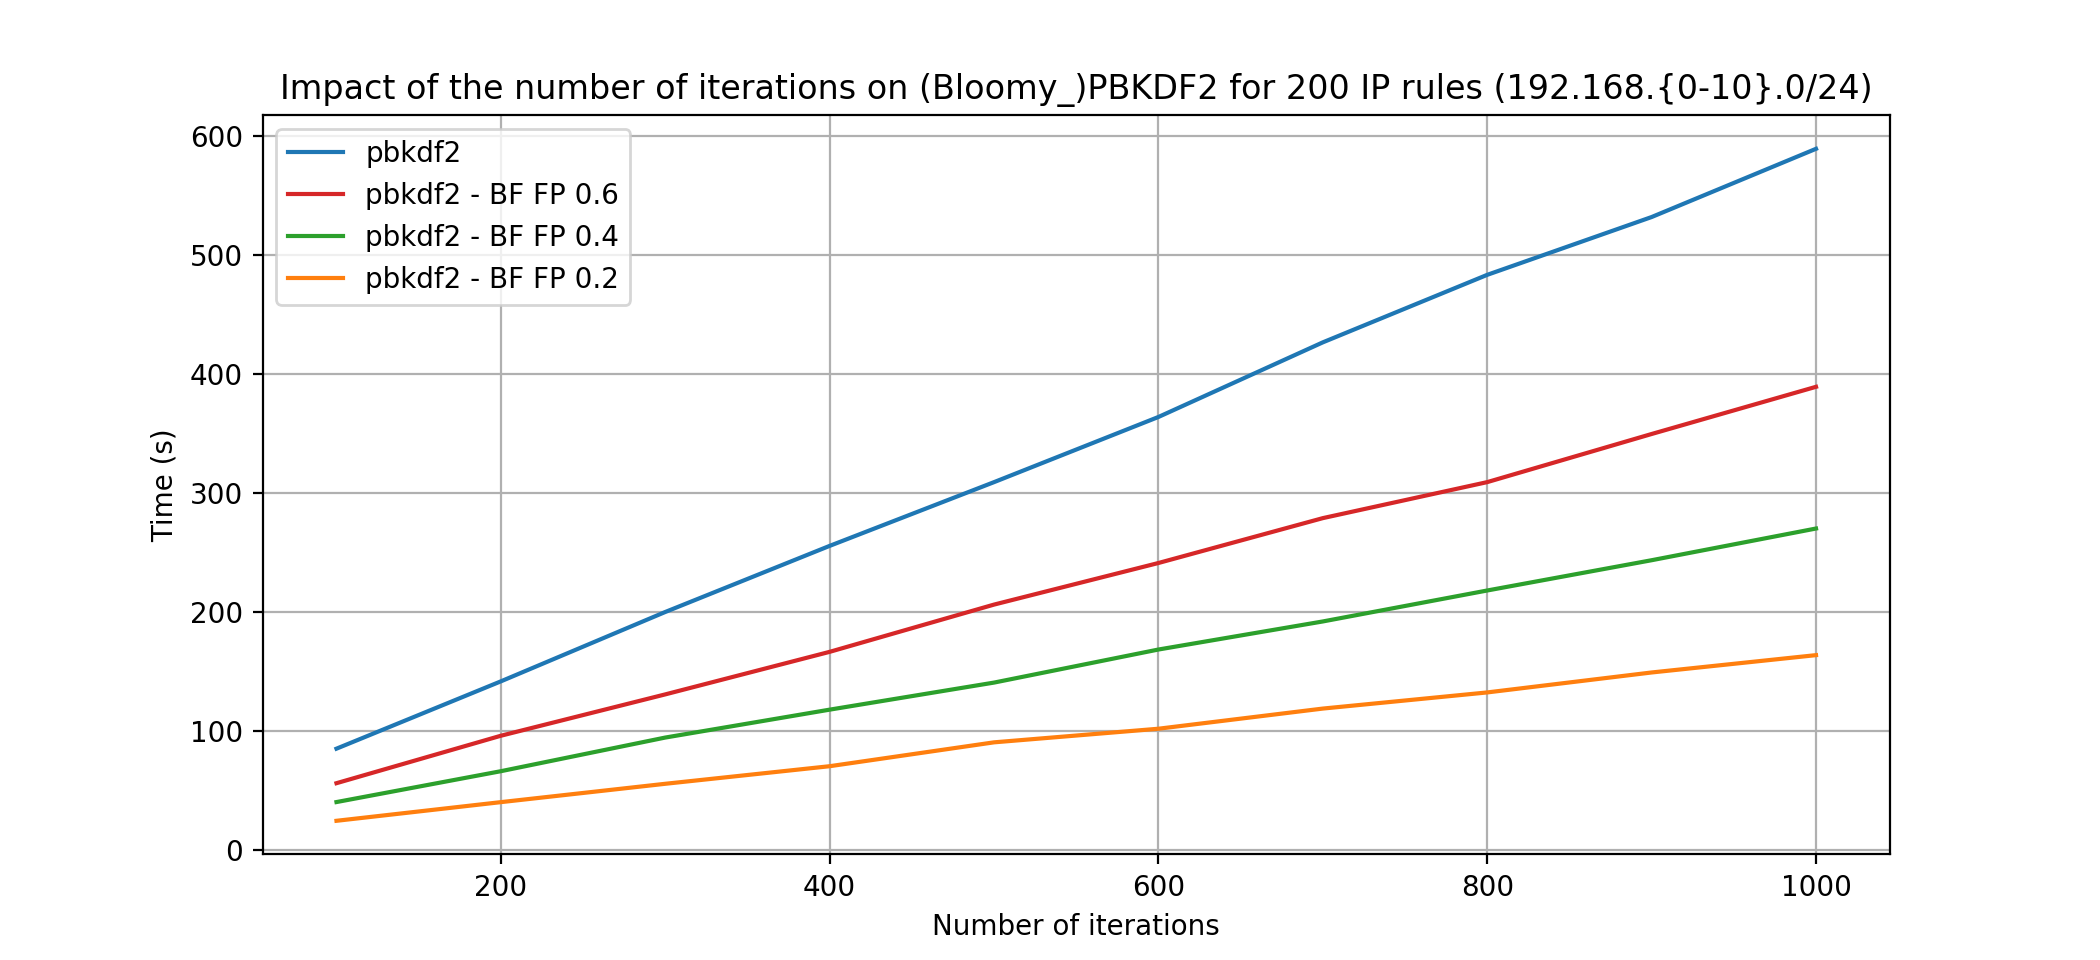
\includegraphics[scale=0.6]{res/TimeIterations}
	\caption{Benchmarking of the evolution of the number of iterations used in the system}
	\label{benchmarking:timeiterations}
\end{center}
\end{figure}

As we can see, the behaviour is effectively similar and the formula could be generalise like:
$$time(nIP, FPrate, nIt, nIPTested)=\left[nIP+(nIPTested-nIP)*FPrate\right]*nIP*nIt*(Time1IP1It)$$

\section{Rules}

The section is intended to give some more technical information about the generated rules.

\subsection{Time for creating a rule}
The major part for generating the rule is the time used by the key derivation function (cfr fig.[\ref{benchmarking:timePBKDF2}, \ref{benchmarking:TimeBcrypt}]). After that, there is a little overhead due to the normalisation and the encryption of the message but they are quickly negligible.\\

\subsection{Space memory consumed by a rule}
Bloom Filters are used to decrease the space memory consumption while memorising the membership of big dataset. Here instead of focusing on that, the goal was to keep every element and transform them in an other format that needs information and cryptographic computations to read them.\\

This lead me to add salts, nonces (IV) and a message on top of that. This has a big impact on memory as the elements are not remembered anymore, but the value is only used to encrypt the message.\\

With that, the size of a rule is nearly a constant as it only depends on the size of the message. For example, the size of a rule for an ip-dst is :
\begin{itemize}
\item[•] Salt (base64): 44 bytes
\item[•] Attribute type ("ip-dst"): 6 bytes
\item[•] Nonce (base64): 24 bytes
\item[•] Ciphertext Check (base64): 24 bytes
\item[•] Ciphertext (base64 with message uuid event\_id date): varies with the id size but around 24 bytes
\end{itemize}
This means that we are around 122 bytes by elements plus the size consumed by the Bloom Filter which depends on the \gls{fp}rate used as well as the number of elements. This is huge compared to the size of an \gls{ipv4} address but is still less than some \gls{url}s.

\subsection{Lookup}
The major part of the lookup time is related to the number of rules of the type searched as well as the algorithm used with its cost. And the final cost is trying to decipher the ciphertext check element.\\
Then a simple approximation could be made with the section \ref{sec:KeyDerivationFunction}:
\begin{itemize}
\item[\gls{pbkdf2}] $$Nb\ rules * Nb\ Iterations * 10^{-6}s + Nb\ rules * Time\ AES$$
\item[Bcrypt]  $$Nb\ rules * Nb\ Iterations * 5 * 10^{-3}s + Nb\ rules * Time\ AES$$
\end{itemize}

\subsection{Bruteforce}
Bruteforcing is the original problem that this work is trying to face. For \gls{ipv4} the bruteforce is feasible as the number of different IPs is limited. Therefore we can only use this system to make it harder for an attacker to bruteforce the whole dataset.\\
The following approximation should be taken with care as it follows from a lot of different really strong hypotheses:
\begin{itemize}
\item[•] The attacker tests all non reserved addresses incrementally.
\item[•] The number of \gls{ipv4} in MISP is about 50 000 (not the real number).
\item[•] The number of non reserved \gls{ipv4} addresses is about 592 708 864 ($\approx$13.8\% of the 4 billions possible \gls{ipv4}).
\item[•] Every non reserved \gls{ipv4} has the same probability to be in a rule.
\item[•] An \gls{ip} has a validity of 3 months
\end{itemize}
The last hypothesis is just to get an idea of the time the database needs to resists to a bruteforce attack and needs to be modified as all other hypotheses in function of what is needed.\\
The fact that an \gls{ip} could have a time limitation is due to the fact that most of the attacker are using dynamic \gls{ip}s. Thus after a while, even if the attacker does not disappear, the information of its \gls{ip}s could not be right anymore.\\

Now, the goal is to get an estimation of the cost to use for the algorithm if we want the user having a probability of 80\% to have fully discovered the complete set of \gls{ipv4} in the database after 3 months by applying a bruteforce attack.\\
First, I need to find a number of \gls{ip} that the attacker needs to test to have a probability of 0.8 of having discovered the whole set.\\

\todo[inline]{A faire}

Then, I want this number of \gls{ip} x, to take 3 months to be checked. We thus need to find the cost c for PBKDF2 so that c*x *Time1IP1It $\geq$3*31*24*60*60. Where Time1IP1It was found in section \ref{sec:BloomyEfficiency}.\\

\todo[inline]{Get this number}

Finally, we know that we don't have to worried about other kind of data as the complexity of bruteforcing is exponential.\\
Therefore nearly unfeasible to bruteforce. For example, if we take a seven-character alphanumeric password, for each character, there are 26 (alphabet)+26 (ALPHABET) + 10 (0-9) possibilities that gives approximately $(62^7)*Time1IP1It/(60*60*24*31*12)$ years which means that it is already $547.8$ years for Bcrypt.\\
This gives an idea why bruteforce is very difficult against IOCs like \gls{url}s.\\ 

\chapter{Conclusion}

This small chapter is aimed to go through what have been done and what still need to be done.

\section{Further Work}
This section is aimed to give ideas to continue this work. To be honest, I believe this domain so big and interesting that there will always exist possible improvements and new techniques to test. Although, new papers are flowing as well as current researches.\\
On this implementation, the major improvement would be to consider the sightings reporting. This would not be too complicated as information needed to report that an element had be seen already exists in the \gls{misp} \gls{api} but it brings some additional challenges as, how could we ensure not reporting twice the same sighting while still being anonymous in reporting?\\
An idea could be to report the sightings by sending the rule seen. By doing that, the \gls{misp} instance could check the identity thanks to the token in the request, then he could check that the rule correspond to the \gls{ioc} and finally only saving the timestamp and the ciphertext as the identifier.\\
With that, while adding a new sighting, \gls{misp} can avoid adding twice the same, checking that the user is authorized to report a sighting while still preserving its identity from being revealed to other organisations.\\

With the actual implementation additional modules can be easily created to test other techniques of rules generation. The technique that could be the most interesting to implement and to analyse would be a way to avoid parallelisation in the matching process. \\
Now, in the current implementation, if we would like to divide the number of rules in two sets and then to use two "matching process" function on these separate processes, we would get the same result in a nearly twice faster way. To avoid that, and idea could be to make the rules generation dependant on the previously generated rules. This could be easily done like by simply using the decryption of the previous rule in the generation of a new rule.\\
This could make bruteforce even less efficient but it would make really difficult to create the rules as well as for each new rule, we would need to go through all previously generated ones.\\
But in this case, the bloomy implementation could be even more efficient.\\

Besides that, this implementation leaks the number of \gls{ioc}s contained in the system. It is even worst than with bloom filter as in that case, statistic analyses could be done to approximate the number of elements but here we only need to count the number of rules. This leaked information could be minimized with addition of 'false' rules.  These false rules could be generated for example by choosing a random element and creating the rule each time with new salts but instead of encrypting 16 zero bytes before the message, we could use 16 one bytes.\\
Doing that for padding files with rules to always have a multiple of a certain number of rules. Unfortunately, this does not totally hide this information as it would still leaks a range on the number of possible elements.

A last implementation could be to create a plug-in using this system directly inside an existing \gls{ids}.


\section{Conclusion}
This master thesis was working on creating a shareable dataset of threat information while keeping a special focus on need of the combination of trust, privacy and confidentiality.\\
Unfortunately, I had a lot of difficulties starting this project as I had neither the knowledge nor a concrete goal. But now, I can say that it is really amazing to look at all existing ideas and implementations but also that I badly oriented my search at the beginning and even if I found articles, they were not linked to the right subject but just to subject related to it. By luck, putting all them together bring me to succeed in doing what I wanted to do but now that I know better the subject, that I understand the challenges, If I had to start over, I would completely reorient the research thanks to the findings of these the last few months.\\
For searching information on information sharing, the starting point must be to look at existing tools as it shows exactly the challenges as well as how implementations and researches are directed. This is why this awesome list \cite{AwesomeTreat} could be a really nice starting point.\\
While on the other side, for the privacy and confidentiality concerns, all needed information and researchs are directly linked to \gls{pprl} and the previously cited state of the art \cite{vatsalanprivacy} gives all needed information.\\

This master thesis is thus related to those two broad domains by taking a different approach lead by the paper \cite{van2016private}. I brought with this work an improvement of this proof of concept technique as well as a real implementation on a flourishing open source project called Malware Information Sharing Platform and Threat Sharing (\gls{misp}).\\
This implementation succeeded in creating dataset of Indicator Of Compromise (\gls{ioc}) that can be generated on demand for a specific user. it respects most privacy and confidentiality concerns by obfuscating the data while still allowing it to be decrypted only if the targeted user has the need of the information or information that could enrich analyses.\\
Matching a specific \gls{ioc} then gives the user the identifier of the information in \gls{misp} and, he could then ask permission to access the instance (If the information belongs to another instance) as well as perhaps the permission to get to know the organisation that had seen the indicator.
One other major advantage of this implementation is also this relaxation in the needed trust for sharing due to the idea of Kim van de Kamp et al. to add an identifier of the user inside the key generation. Thanks to that, the risk of leakage is decreased as the source of the leakage could be identified.\\


\printglossary

\bibliographystyle{acm-doi}
\bibliography{articles}
\newpage

% Back cover page
\backcoverpage




\end{document}
